% =====================================================================
% LaTeX Template for the International Journal of Disaster Risk Reduction
% Author: Alexandre Dunant
% Based on Elsevier's elsarticle class
% =====================================================================

\documentclass[preprint,12pt,authoryear]{elsarticle}

% -------------------- PACKAGES --------------------
\usepackage[utf8]{inputenc}
\usepackage[T1]{fontenc}
\usepackage{lmodern}
\usepackage{amsmath,amssymb}
\usepackage{graphicx}
\usepackage{booktabs}
\usepackage{caption}
\usepackage{subcaption}
\usepackage{url}
\usepackage{hyperref}
\usepackage{lineno}
\usepackage{xcolor}
\usepackage{float}


% -------------------- SETTINGS --------------------
\linenumbers                    % Enable line numbers for review
\journal{International Journal of Disaster Risk Reduction}

% Hyperref setup
\hypersetup{
    colorlinks=true,
    linkcolor=blue,
    citecolor=blue,
    urlcolor=blue,
    pdftitle={Multi-hazard scenario ensembles for estimating earthquake risk},
    pdfauthor={Alexandre Dunant}
}

% Bibliography style: author-year
\bibliographystyle{elsarticle-harv}

% -------------------- DOCUMENT --------------------
\begin{document}

\begin{frontmatter}

\title{Multi-hazard scenario ensembles for estimating earthquake risk}

\author[inst1,inst2]{Alexandre Dunant\corref{cor1}}
\author[inst3]{Tom R. Robinson}
\author[inst1]{Alexander L. Densmore}
\author[inst4]{Sweata Sijapati}
\author[inst1]{Nick J. Rosser}
\author[inst5]{Mark Kincey}
\author[inst6]{Katie J. Oven}
\author[inst7]{Stine Heiselberg}
\author[inst7]{Ragindra Man Rajbhandari}



% Use \cortext for the corresponding author details
\cortext[cor1]{Corresponding author; now at EURAC, Bolzano, Italy. Email: Alexandre.dunant@eurac.edu}

% Define the addresses using the [instX] labels
\address[inst1]{Institute of Hazard, Risk, and Resilience and Department of Geography, Durham University, Durham, UK}
\address[inst2]{Center for Climate Change and Transformation, EURAC, Bolzano, Italy}
\address[inst3]{School of Earth and Environment, University of Canterbury, Christchurch, New Zealand}
\address[inst4]{National Society for Earthquake Technology, Kathmandu, Nepal}
\address[inst5]{School of Geography, Politics, and Sociology, Newcastle University, Newcastle, UK}
\address[inst6]{Department of Geography and Environmental Sciences, Northumbria University, Newcastle, UK}
\address[inst7]{UN Resident Coordinator's Office, Kathmandu, Nepal}

\begin{abstract}
Anticipating the likely impacts of a future large earthquake is essential for effective humanitarian contingency planning. Ideally, that planning should incorporate both the range of potential future earthquake locations and magnitudes, and earthquake-related secondary hazards - which in many continental settings includes coseismic landsliding. Here, we extend a previously-developed earthquake scenario ensemble approach to explicitly include coseismic landsliding using a hypergraph network model to quantify multi-hazard risk across the ensemble. We apply this model to a set of 30 plausible large-magnitude ($M_w > 7$) earthquakes across Nepal to evaluate the combined impacts of shaking and landsliding on buildings and road infrastructure. While shaking damage dominates the overall impact profile, our findings reveal that landslides substantially increase impacts in steep and remote regions, where landslide impacts on buildings and roads can exceed $\text{50\%}$ of the number of buildings directly damaged by shaking. The results show a strong and statistically significant correlation between district remoteness and the proportion of road segments damaged by landslides (Spearman $\rho = 0.81$), which compounds the challenges of emergency response and of access to health care and government facilities. These findings are consistent with an urban-rural risk divide shaped by Nepal's diverse topography, in which densely populated urban and lowland districts face the largest absolute numbers of buildings damaged by shaking, while remote hill and mountain districts face the highest proportional impacts and the greatest likely challenges to post-earthquake access. This multi-hazard ensemble approach provides a more comprehensive understanding of earthquake risk than shaking-only assessments, offering valuable insights for contingency planning by humanitarian organisations and the Government of Nepal.
\end{abstract}

\begin{keyword}
cascading multi-hazards \sep multi-hazard modelling \sep earthquake scenarios \sep earthquake impacts \sep landslides \sep Nepal \sep network modelling
\end{keyword}

\end{frontmatter}

% -------------------- MAIN TEXT --------------------

\section{Introduction}
Earthquakes have killed more than two million people since 1900 \citep{England2011,Daniell2017} and remain one of the deadliest global hazards. Humanitarian contingency planning for future earthquakes, which comprises both preparation for earthquake response as well as pre-emptive efforts to reduce the impacts from a future earthquake \citep{IASC2007,IFRC2012}, is most likely to be effective if it is based on the best available scientific information on the associated risks \citep{Alexander2007}. This information should ideally include estimates of the scale of impacts in a future earthquake as well as the locations where those impacts are most likely to occur \citep{IASC2007}.

In contingency planning, the emphasis is typically placed on preparing for a single scenario, such as the worst-case or `maximum credible event', or the recurrence of a large historical earthquake under present-day conditions \citep[e.g.,][]{klugel_seismic_2008}. It can be useful, however, to distinguish between a range of possible or plausible impacts, especially when planning involves the allocation of often scarce resources \citep{Robinson2018}. Existing approaches to seismic risk analysis typically fall into one of two categories \citep{Robinson2018, mcguire_deterministic_2001}. Deterministic approaches use scenarios that precisely define the effects of one or a small number of possible future earthquakes \citep{Davies2015}, often chosen as the maximum credible event that could be expected on a particular fault, or as a design event with a specified probability of exceedance over the lifetime of the assets being considered (commonly 10\% in 50 years). In contrast, probabilistic approaches rely on estimates of the likelihood of exceeding a given value of ground motion from all possible seismic sources over a specified period of time, with the corresponding impacts from that level of shaking representing the total cumulative losses over the time period.

Building upon a body of work that has critically reviewed both probabilistic and deterministic approaches \citep{Bommer2002,Wang2003,Wang2011,Bilham2013, klugel_seismic_2008}, Robinson et al. \citep{Robinson2018} noted that, for many of the world's earthquake-prone areas, there are insufficient data on past earthquakes and their impacts to reliably apply either method. Borrowing from common practice in climate modelling, they proposed an alternative approach that used an ensemble of earthquake scenarios to identify emergent patterns of impacts. This allowed them to distinguish between consequences that were common across multiple scenarios -- and thus, when the relative likelihoods of the scenarios are unknown, more likely to occur in future -- from those that were highly specific to an individual future event \citep{Robinson2018}. They applied this ensemble approach to evaluate relative earthquake risk in Nepal to support contingency planning by the humanitarian clusters of the UN Humanitarian Country Team and the Government of Nepal. Importantly, because the annual probability of each of the different scenarios were equally weighted in the ensemble, they focused exclusively on relative risk between scenario outcomes, rather than absolute risk. This approach now forms the basis of the current earthquake emergency response and preparedness plan in Nepal \citep{un_nepal2022earthquake}.

An important shortcoming of the scenario ensemble developed by Robinson et al. \citep{Robinson2018}, however, is that it only considered direct damage to buildings resulting from earthquake shaking. Experience in recent large continental earthquakes shows that shaking damage is only one part of a common chain of earthquake-triggered secondary hazards \citep{Gill2014}. Landslides, debris flows, sediment aggradation, and subsequent flooding can have persistent impacts over years or even decades after the earthquake \citep{Fan2019,Kincey2021, francis_fate_2022}. It has also been noted that earthquakes that trigger landslides typically cause more fatalities than those that do not \citep{Budimir2014}. Planning for future earthquake impacts in continental settings should therefore account for this wider range of earthquake-related hazards.

Promisingly, multi-hazard approaches to risk assessment are now becoming more widespread (see recent reviews by \cite{Gill2022,Ward2022}). Multi-hazards are defined by UNDRR (\url{https://www.undrr.org/terminology/hazard}) as "events [that] may occur simultaneously, cascadingly or cumulatively over time, and [that take] into account the potential interrelated effects". However, while many "multi-hazard" risk models overlay single hazards without considering their interactions \citep{Gill2014}, there is growing recognition that true multi-hazard risk assessment requires models that can consider interactions, and capture spatial clustering and  amplification effects \citep{Mignan2014,Tilloy2019,Dunant2021,Ming2022,Hochrainer-Stigler2023}.

Dunant et al. \citep{Dunant2025} proposed a novel multi-hazard impact model that used a hypergraph framework to link elements at risk -- such as buildings or roads -- within spatial domains that correspond to the areas exposed to a hazard such as an earthquake. The hypergraph approach allowed efficient estimation of the impacts from cascading multi-hazards; in turn, this efficiency meant that the impacts of a scenario earthquake could be simulated repeatedly within a Monte Carlo framework to derive statistical estimations of the areas most likely to be affected. They evaluated the model against the 2015 Mw 7.8 Gorkha earthquake in Nepal, and showed that the model could reasonably approximate the spatial patterns of building damage due to shaking as well as building and road damage due to earthquake-triggered landslides.

Here, we apply the multi-hazard impact model of Dunant et al. \citep{Dunant2025} to the scenario ensemble analysed by Robinson et al. \citep{Robinson2018}, in order to provide the first quantitative estimates of a suite of potential multi-hazard impacts arising from the next earthquake to occur in Nepal. This provides a substantially more complete picture of both the number and spatial distribution of earthquake-related impacts, including those arising from earthquake-triggered landslides than was previously possible. Our purpose is not to predict the specific details of a future earthquake. Instead, we aim to illustrate the range of potential impacts that could arise from a suite of plausible earthquake scenarios, and the areas most likely to be affected by earthquake shaking and earthquake-triggered landslides, in order to support and inform contingency planning by the Humanitarian Country Team and the Government of Nepal \citep{Sijapati2024}.

\section{Methods}
We first provide a brief overview of the hypergraph multi-hazard impact model and its key assumptions, including the sources of variability in its outputs (Section~\ref{sec:model}). We then describe the earthquake scenario ensemble that we use to drive the model (Section~\ref{sec:ensemble}), and the experimental setup and data sources, where the treatment of shaking and landslide impacts used in this study is described in more detail (Section~\ref{sec:setup}). Finally, we describe the analysis of the ensemble outcomes (Section~\ref{sec:analysis}) and the multi-hazard risk scores (Section~\ref{sec:riskscores}).

\subsection{Model description}
\label{sec:model}

A full description of the hypergraph multi-hazard impact model is provided by Dunant et al. \citep{Dunant2025}, along with details of its application to the 2015 Mw 7.8 Gorkha earthquake. Here, we give an overview of the model and its key assumptions; the implementation of each step is then described in more detail in Section~\ref{sec:setup}. The model operates on a network of nodes, each of which represents either a hillslope or an asset at risk. Hillslopes are represented by individual slope units, which are terrain units bounded by drainage and divide lines \citep{Alvioli2016}, and assets are, in this case, buildings and road segments. These nodes are connected by hyperedges, which can be thought of as polygons that enclose one or more nodes. Unlike edges in graph-based models, which link a single pair of nodes \citep{Dunant2021}, hyperedges can connect multiple nodes. For example, in the model used here, one of the hyperedges links all slope units, defining them as lying within Nepal. Those slope units, in turn, can be represented by individual hyperedges that link all of the buildings and roads on each hillslope. In this way, we can define a nested set of hyperedges that preserve both the characteristics of each node -- for example, the topography of each slope unit, or the building type, or the susceptibilities to landslides or debris flows at each building location -- and the spatial relationships between those nodes. The efficiency of the hypergraph network means that hundreds or thousands of separate simulations can be run for each earthquake scenario, with each simulation exploring a different pathway through the network of possible cascading impacts \citep{Dunant2025}. A Monte Carlo approach allows us to represent the uncertainty within a single scenario by repeatedly sampling the stochastic components of the model to generate a statistical distribution of possible outcomes \citep{dunant2021multihazards}, from which we derive the likelihood that each asset -- that is, each building or road segment -- is affected. In the implementation used here, these stochastic components are the random draws that determine, in each model run, whether the slope unit containing a given asset is activated by the earthquake shaking, whether a landslide is triggered within that slope unit, and whether that landslide impacts the asset (Section~\ref{sec:setup}). By contrast, the PGA field of each scenario earthquake is fixed, and the likelihood of complete damage to a building by shaking is taken directly from the fragility functions, so it does not vary between runs. By applying this process to each earthquake from an ensemble of plausible scenarios, we also capture inter-scenario variability, and could in principle assess the degree to which the range of outcomes for one scenario overlaps with those of others. In this study, however, we summarise the within-scenario distribution by its expected value, that is, the mean number of damaged assets per model run, averaged over the 10,000 runs of that scenario (and not across scenarios). The variability we report therefore reflects differences in impacts between possible future earthquakes. The within-scenario spread of outcomes is not propagated into the results presented here because, unlike the expected value, it depends strongly on how outcomes are correlated between neighbouring assets -- for example, when several buildings are affected by the same landslide -- which is not well constrained (Section~\ref{sec:limitations}).

The implementation of the model is focused on the chain of hazards associated with large continental earthquakes \citep{Fan2019}. Earthquake shaking is assumed to cause direct damage to buildings as defined by a set of fragility functions that relate peak ground acceleration (PGA) to the probability of reducing the building to a complete damage state for the range of typical building types in Nepal (Figure S1). Shaking can also trigger landslides within individual slope units, with a probability that increases with the PGA in each slope unit (Section~\ref{sec:setup}), and those landslides may in turn intersect, and thus impact, buildings or road segments within the slope unit. Unlike shaking damage, which is estimated through fragility functions that account for the vulnerability of each building type, landslide impacts are based on the co-location of an asset with a modelled landslide, without a corresponding damage-state (vulnerability) function; we assume that any building or road segment impacted by a landslide is damaged, and refer to such assets as `damaged by landslides' below. Because our focus is on the direct impacts of our chosen scenario earthquakes, we do not consider longer term or delayed hazards such as landslide reactivation by subsequent rainfall \citep{Fan2019,Kincey2021}, or consequent downslope changes in sediment storage and flood capacity. Thus, our results should be interpreted as reflecting the main instantaneous coseismic effects that could be observed immediately after the earthquake. Other hazards, such as those triggered directly by rainfall, are also not considered, although they could be added via additional sets of hyperedges and interactions.

To generate a single earthquake impact scenario, we apply the expected ground shaking in terms of PGA (g) from our chosen earthquake, modelled as described in Section~\ref{sec:ensemble}, to the hypergraph model and evaluate 10,000 separate outcomes from that event -- that is, we repeat the hypergraph model 10,000 times, each time following a separate path through the hypergraph network as a result of the random draws described above. This generates a distribution of model outcomes in terms of the likelihood that any building will be damaged by earthquake shaking or by landsliding, and the likelihood that any 100 m road segment will be damaged by landsliding. Those likelihoods can then be aggregated to identify the areas most likely to be affected by one or another of those components in the earthquake hazard chain. Aggregation can be carried out over any spatial unit, such as administrative units, grid cells or catchments, but is needed to obtain robust results, because the performance of the model improves as the likelihoods for individual assets are aggregated over larger areas \citep{Dunant2025}. Here, we aggregate by district, which also matches the scale at which contingency planning is carried out in Nepal and avoids implying a false level of precision (Section~\ref{sec:analysis}). We then repeat this process for the other scenario earthquakes, and examine the ensemble of outcomes that result.

\subsection{Earthquake ensemble}
\label{sec:ensemble}

Robinson et al. \citep{Robinson2018} assembled an ensemble of 30 large ($M_w > 7$) earthquakes that could plausibly cause damage in Nepal and that would warrant at least a national-scale response, based on a combination of historical records and palaeoseismic evidence along with the distribution of major faults (Figure~\ref{fig:study}). These included earthquakes along the Main Himalayan Thrust, ranging in magnitude from $M_w$ 7.3 to 8.6, as well as earthquakes in the upper plate of the Main Himalayan Detachment on the Karakorum Fault ($M_w$ 7.8), the northern ($M_w$ 7.8) and southern ($M_w$ 7.3) parts of the Western Fault System, and the Thakkhola Graben ($M_w$ 7.3). For direct comparison of our modelling with their results, we adopt the same 30 scenario earthquakes. The pattern of PGA for each of these 30 events was modelled with OpenSHA \citep{Field2003}, using the ground motion prediction equations of Abrahamson and Silva \citep{Abrahamson2008}, exceedance probabilities of $\text{50\%}$, and shallow shear wave velocity (Vs30) derived from topographic slope \citep{Allen2009}. Maps of PGA for each of the 30 scenario earthquakes are shown in Figure \ref{fig:S2}.

\begin{figure}[H]
    \centering
    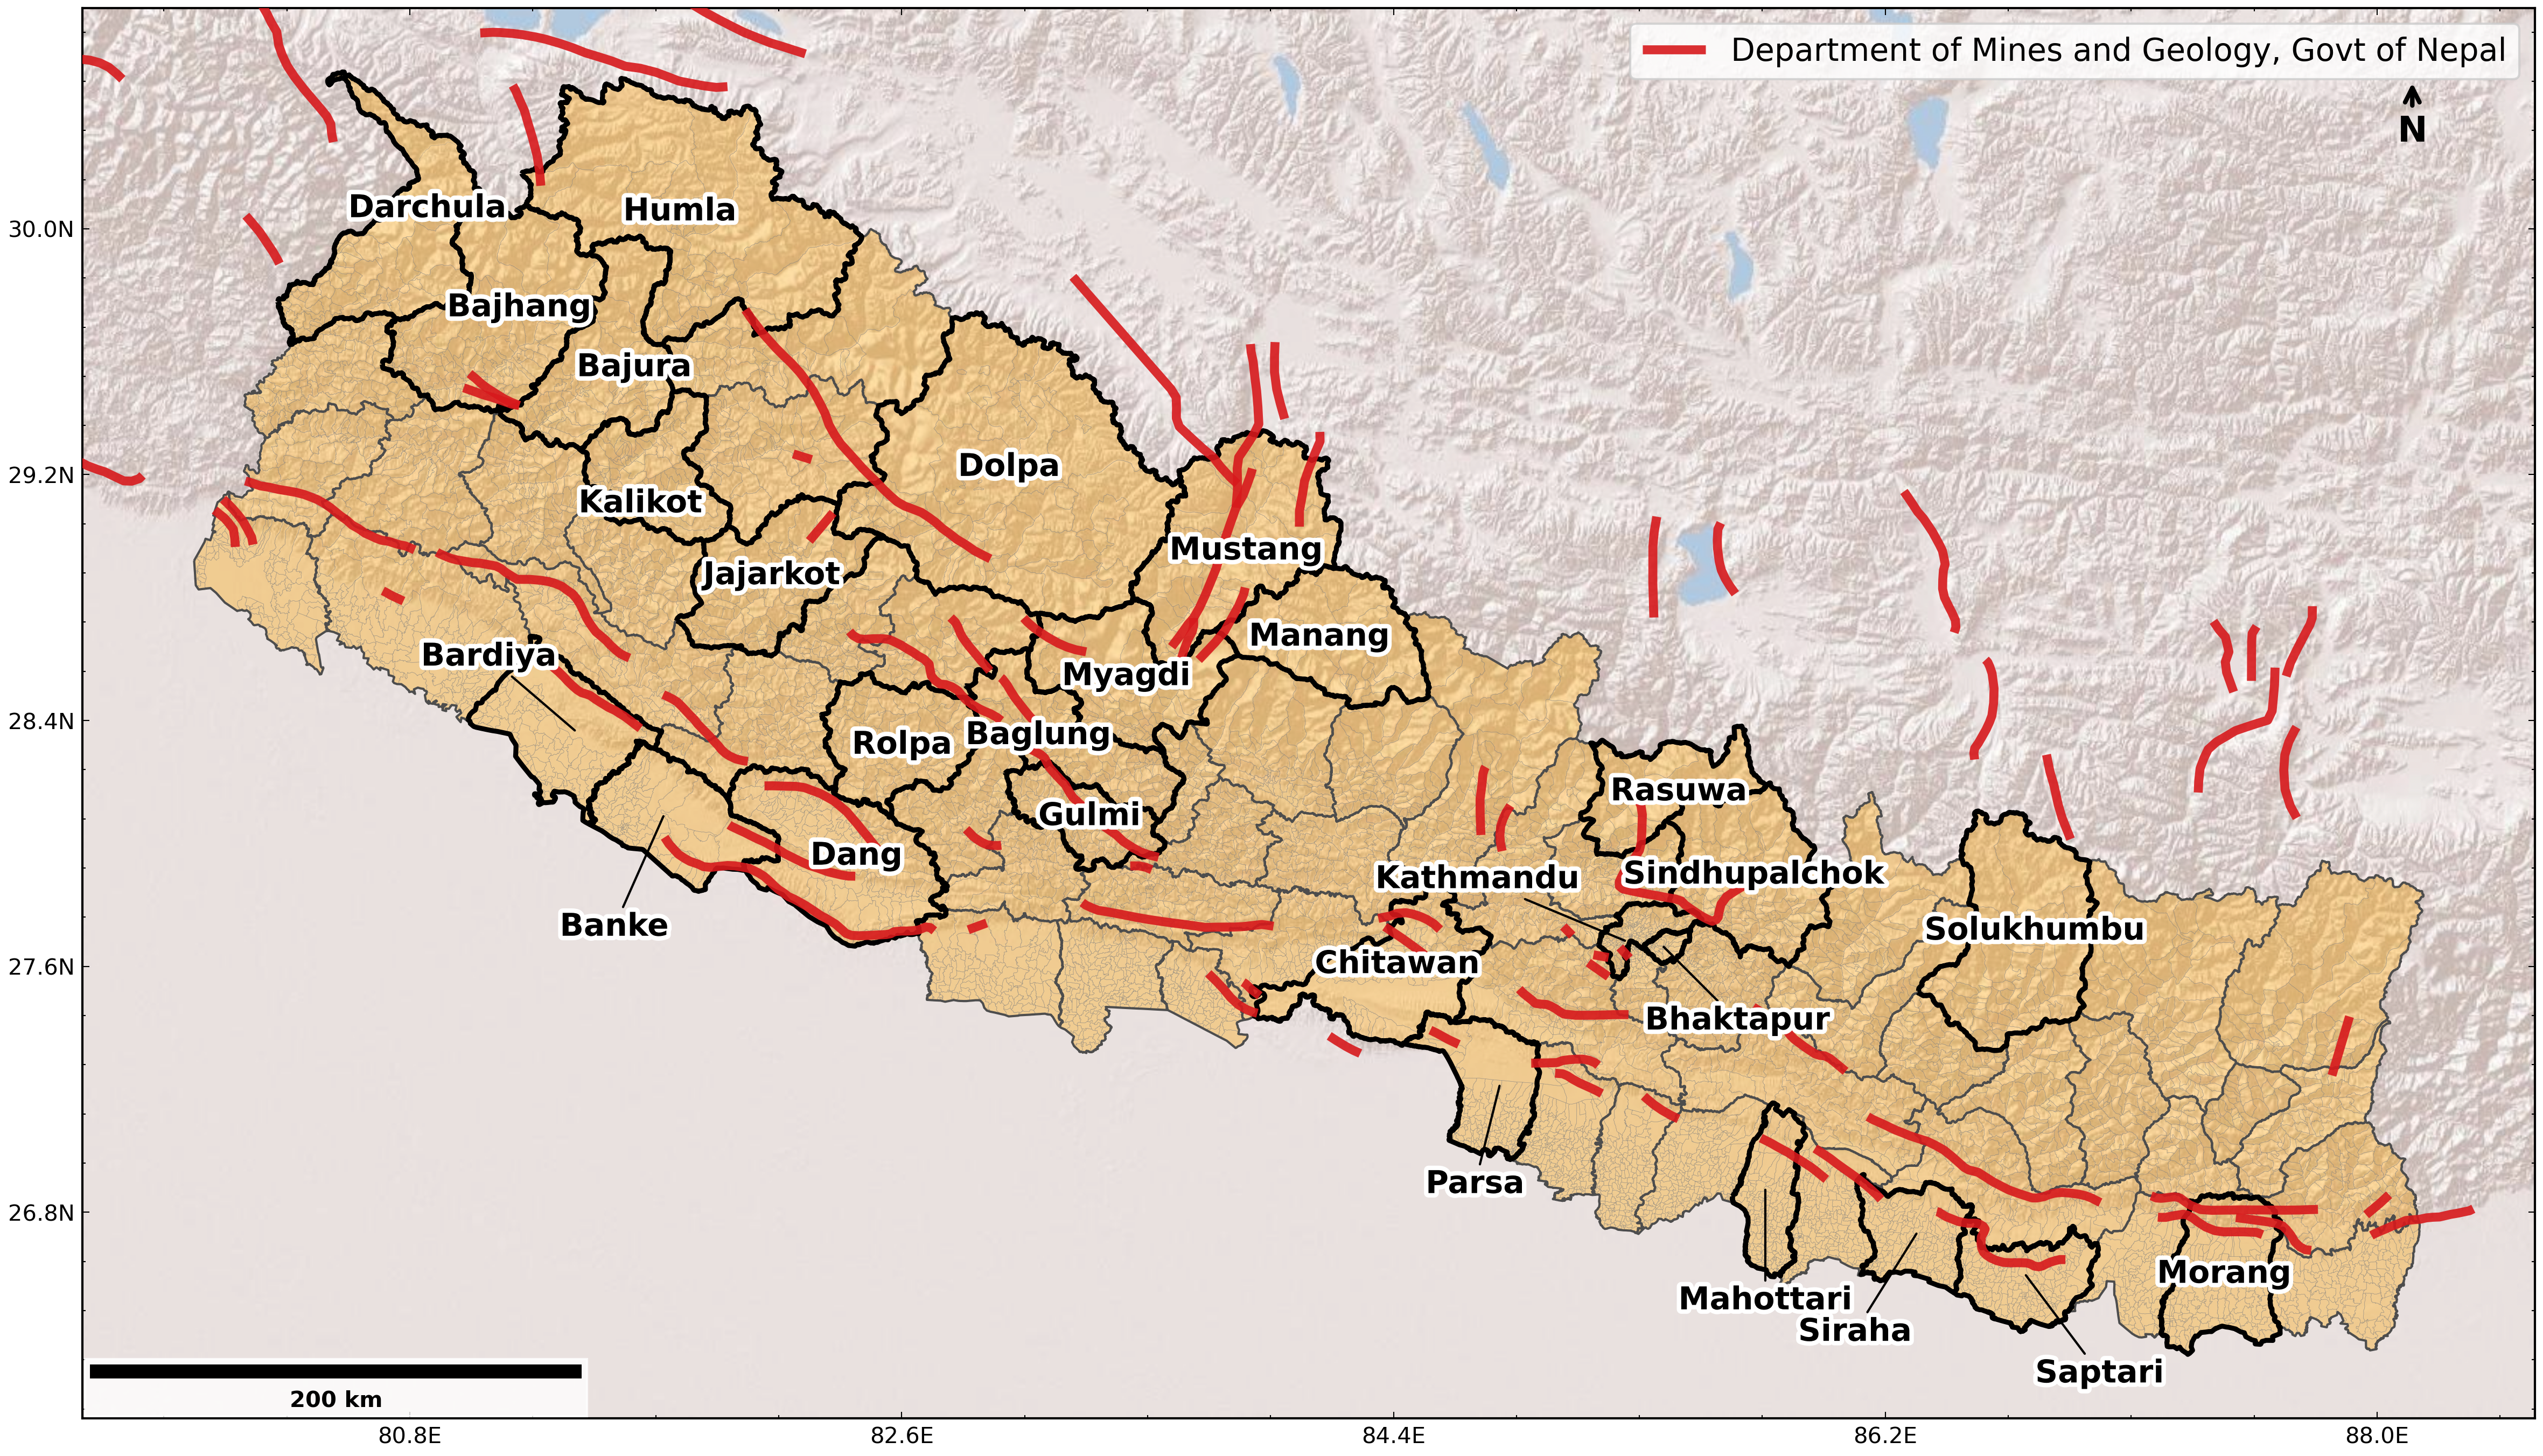
\includegraphics[width=1\linewidth]{./FIGURES/revised_v2/Fig1_study_area_map.png}
    \caption{Map of districts and major fault systems in Nepal. Fault traces are sourced from the Department of Mines and Geology, Government of Nepal. Districts discussed in the text are outlined and labelled; all 77 districts are named in the Supplementary Information.}
    \label{fig:study}
\end{figure}


\subsection{Experimental setup and data sources}
\label{sec:setup}

For each scenario earthquake, the model proceeds through the hyperedges that connect earthquake shaking to other nodes in the model, checking to see whether each hyperedge is 'activated' -- that is, whether a building is damaged by shaking or a slope unit is affected by one or more landslides. If that hyperedge is activated, then the simulation propagates along that hyperedge and can cascade to other hyperedges through the network.

We first check the buildings within the footprint of the earthquake (defined by a PGA cutoff value of $0.1\,\text{g}$, below which the probability of complete damage is low for all building types; see Figure \ref{fig:S1}). We use building locations taken from the Humanitarian OpenStreetMap Team available from \url{https://data.humdata.org/dataset/hotosm_npl_buildings} (last accessed \textcolor{red}{[DATE]}), comprising approximately 7.1 million building polygons. Road polyline data are taken from the same source (\url{https://data.humdata.org/dataset/hotosm_npl_roads}; last accessed 1 January 2021) and were divided into $100\,\text{m}$ segments, giving approximately 3.2 million road segments \citep{Dunant2025}. Construction types are not available for individual building polygons, so we use the best-available national-scale exposure data from the Modelling Exposure Through Earth Observation Routines (METEOR) project, available from \url{https://maps.meteor-project.org/map/building-exposure-map-of-nepal} (last accessed \textcolor{red}{[DATE]}). This dataset provides the relative proportions of different building types within each $90 \times 90\,\text{m}$ grid cell. For each building type, we define three separate fragility functions -- a `Low', `Mid', and `High' case -- representing the uncertainty in structural performance (Figure \ref{fig:S1}). We then generate a single, representative fragility function for each grid cell by calculating a weighted average of these functions, where the weights are determined by the proportions of each building type in that cell. We then compare the weighted-average fragility function in each cell to the PGA value at the cell centroid to determine the likelihood of complete damage for each building $[0,1]$ for the low-, mid- and high-fragility cases. Dunant et al. \citep{Dunant2025} showed that the mid-fragility case was best able to reproduce observed building damage patterns and numbers in the 2015 Gorkha earthquake, so here we focus on the results with the mid-fragility case below.

For each slope unit, we compute the mean PGA value and use it to determine the probability of landsliding based on a lognormal function that is calibrated by observations in the 2015 Gorkha earthquake \citep{Dunant2025}. We then compare this probability against a uniform random deviate to determine whether a slope unit is activated during a simulation. Over multiple simulations, slopes that were more likely to experience a landslide will be activated more frequently. However, due to the probabilistic nature of this approach, the exact pattern of activations can vary between simulations. For each slope unit that is activated, the model proceeds to determine whether landslides are triggered and, if so, whether they impact buildings or road segments within that unit. To do so, we evaluate landslide susceptibility using a model that relies exclusively on static topographic variables (i.e., no earthquake-specific information). This model incorporates seven key factors: elevation, hillslope aspect, proximity to rivers, plan-view curvature, regional relief, local slope gradient, and a terrain ruggedness index. These factors are derived from a $10\,\text{m}$ resolution digital elevation model (DEM), which was created by downsampling the $5\,\text{m}$ DEM provided by the Advanced Land Observing Satellite World 3D (\url{https://www.aw3d.jp/en/products/standard/}). We applied the XGBoost machine learning algorithm, implemented in Python, to develop the susceptibility model \citep{Dunant2025}. For the purposes of this study, the model was trained using data from coseismic landslides triggered by the 2015 Gorkha earthquake, as documented by Kincey et al. \citep{Kincey2021}. The model achieved an area under the receiver operating characteristic (ROC) curve of $0.75$. It should be emphasised that this susceptibility model is optimised for the 2015 Gorkha earthquake, and it would be possible to use other susceptibility models within the hypergraph framework as required.

Whether or not a landslide is triggered in a slope unit is determined by drawing a value from a Gaussian distribution of landslide susceptibility with the same mean and standard deviation as the distribution of susceptibility values in that slope unit, and comparing that value with a uniform random deviate \citep{Dunant2025}. If the susceptibility value is smaller than the random deviate, then no landslide occurs and propagation along that hyperedge stops. If a landslide is triggered in a given slope unit, we perform a secondary check to assess whether individual buildings and road segments within that unit are impacted. This is done by comparing the landslide susceptibility value at the location of each asset (representing potential impact probability) with a uniform random deviate. If the deviate exceeds the susceptibility value, the asset is considered unaffected; otherwise, we assume it is impacted by the landslide. This check is applied to all buildings in the slope unit, irrespective of their likelihood of being damaged by shaking. While the slope unit-scale susceptibility governs the triggering of landslides, the local susceptibility value at each asset location is used as a proxy for spatially-variable impact likelihood. Because the susceptibility model is trained on the full footprint of coseismic landslides \citep{Kincey2021}, this impact likelihood encompasses both source and runout areas. This process is repeated iteratively across all activated slope units to generate a cascading impact scenario, simulating the spread of landslides and their effects on infrastructure throughout the region. We continue this process iteratively to search through all slope units in the network to generate a single outcome for that earthquake. This is repeated 10,000 times for each scenario earthquake. This results in a shaking impact likelihood and a landslide impact likelihood, both in the range $[0,1]$, for each building, and a landslide impact likelihood in the range $[0,1]$ for each $100\,\text{m}$ road segment in our national-scale dataset. The two building likelihoods are calculated independently and are not mutually exclusive, as a building can be both damaged by shaking and impacted by a landslide. They also represent different components of risk: the shaking likelihood combines hazard intensity (PGA) with building vulnerability (the fragility functions), whereas the landslide likelihood reflects the probability that a landslide reaches the building, without a measure of vulnerability (Section~\ref{sec:model}). We therefore report the two separately, rather than combining them into a single probability of damage for each building. Finally, we move on to the next earthquake in the 30-member ensemble and repeat the steps above.

\subsection{Analysis of ensemble outcomes}
\label{sec:analysis}

Robinson et al. \citep{Robinson2018} focused on scenario earthquake impacts in terms of fatalities, using statistical relationships between building damage states, building occupation rates, and fatality rates. Because occupation rates vary over time (e.g., between day and night), they also considered three possible occurrence times for each of the 30 scenario earthquakes. Here, we focus instead on earthquake impacts on static assets only (buildings and roads), both through shaking and earthquake-triggered landsliding, and so we limit our analysis to the 30 earthquakes without considering occurrence time. Extending our multi-hazard results to estimate fatalities would require well-established empirical functions to relate landslide occurrence to fatality rates for both people in buildings and those using the road network \citep{VanWykDeVries2024}. Research on this topic remains limited, and the relationships proposed to date \citep{Pollock2020,Luo2023,Hu2024} are too scattered and uncertain to be applied with confidence in settings comparable to that studied here. Our choice to focus on the impacts to infrastructure is justified also by the common need in humanitarian contingency planning to focus on the numbers of affected households who will potentially require assistance \citep{IASC2007,Sijapati2024}. The detailed relationship between the locations of infrastructure, which are typically known, and the locations of people in the landscape over time, which are typically not known, remains an outstanding gap, and we return to this point in the discussion.

While the hypergraph model generates an impact likelihood for each building and each $100\,\text{m}$ road segment in our infrastructure database, this is only valid in a probabilistic sense and does not represent a statement that `building X will be damaged in earthquake N'. As noted in Section~\ref{sec:model}, the model outputs therefore need to be aggregated: \cite{Dunant2025} showed that the performance of the hypergraph model improved as model results were aggregated over increasingly large administrative areas when simulating the 2015 Gorkha earthquake. They identified the district level ($n = 77$ in Nepal; Figure~\ref{fig:study}) as providing the optimum trade-off between model performance and granularity of results, which is also the resolution preferred by the humanitarian clusters for contingency planning in Nepal \citep{Sijapati2024}. Nepal's districts have a mean area of about 1,900~km$^2$, ranging from about 120~km$^2$ (Bhaktapur) to about 8,000~km$^2$ (Dolpa). Although many of their functions were transferred to provincial and local governments under the federal structure introduced by the 2015 constitution, districts retain a coordinating role, and district-level bodies such as the District Disaster Management Committees remain important for disaster management \citep{Bhandari2020}. Accordingly, we primarily aggregate our results at district level in the sections below. We do this by calculating the expected number of (1) buildings damaged by earthquake shaking, (2) buildings damaged by coseismic landsliding, and (3) road segments damaged by coseismic landsliding, taking each as the sum of the per-building (or per road segment) likelihood values in that district. For example, if a district contains 60,000 buildings and the mean per-building likelihood of complete damage by shaking is $0.05$, then on average we would expect 3,000 buildings to be completely damaged in that earthquake. The expected numbers are calculated separately for each type of impact; because a building can be both damaged by shaking and impacted by a landslide (Section~\ref{sec:setup}), the expected numbers of buildings damaged by shaking and by landsliding are not mutually exclusive, and their sum is a number of impacts rather than a number of damaged buildings. These district totals do not require damage to be independent between buildings or between road segments, because the expected value of a sum is equal to the sum of the individual expected values, whatever the dependence between them. Spatial correlation (e.g., through co-location on a large landslide mass) would, however, widen the distribution of outcomes around these expected values.

We use the expected numbers of buildings damaged by shaking, buildings damaged by coseismic landsliding, and road segments damaged by coseismic landsliding to estimate the exceedance frequency of impacts across the 30 scenario earthquakes. Because the scenarios are equally weighted and have no associated recurrence rates, this is not a probability of occurrence over time, but the fraction of the 30 scenarios in which a given impact is equalled or exceeded; we therefore refer to it as the scenario exceedance frequency, or simply exceedance frequency, below. This allows us to determine both the median and worst-case for each type of impact within each of Nepal's 77 districts.

We also examine the variability of each of our three types of impact across the different scenarios. If all scenarios result in similar impacts within a district, then the potential impacts are likely to occur irrespective of the details of the next earthquake. Conversely, if the impacts vary greatly between the different scenarios, then there is high uncertainty about what could occur in the next event. To capture this, we calculate, for each district and separately for each of the three types of impact, the standard deviation of damage across the 30 scenario earthquakes. A high standard deviation indicates that the number of damaged assets depends strongly on which earthquake occurs, whereas a low standard deviation suggests a more consistent impact profile regardless of the specific event. Because it is expressed in numbers of assets, the standard deviation also scales with the number of exposed buildings or road segments; it therefore describes the absolute spread of damage that contingency plans may need to accommodate, rather than a relative measure of variability. For comparison, we also map the coefficient of variation (the standard deviation divided by the mean) across the 30 scenario earthquakes, which does not depend on the number of exposed assets and indicates how variable impacts are relative to their typical level.

\subsection{Multi-hazard risk scores}
\label{sec:riskscores}

To extend our analysis to multi-hazard risk and identify districts where risk is specifically related to one hazard type or where risks from different hazards combine, we develop two multi-hazard risk scores. Both scores incorporate a remoteness factor, which serves as a proxy for the logistical challenges of post-disaster aid delivery. As in the work presented in \cite{Robinson2018}, measures of remoteness are an important component of relative risk because they attempt to account for the time it will take for communities to receive aid after a large earthquake.

We use remoteness index values estimated by \cite{banick2019}, who quantified physical remoteness within Nepal using a geographic information system-based cost-time model that calculated travel times from any location to essential services. They integrated digital elevation data, road networks, land cover, and seasonal conditions to model realistic travel impedance across varied terrain, using a $30\,\text{m}$ resolution raster grid across all of Nepal. Their model accounted for topographic constraints by implementing switchback algorithms for steep slopes, assigned different speeds to four hierarchical road classes, and incorporated seven land cover categories for off-road travel. Seasonal accessibility variations were captured through separate dry and monsoon season models, with appropriate speed reductions applied to different road types during adverse conditions. The resulting travel time estimates were validated by \cite{banick2019} against household survey data and expert consultations, then aggregated by administrative units to produce separate remoteness metrics for the dry and monsoon seasons. Their results specify the fraction of the population, based on the WorldPop 2015 UN-adjusted population density dataset at $100\,\text{m}$ resolution, in each administrative unit for whom essential services can be accessed within one of eight time intervals ($0$--$30$ minutes, $30$ minutes--$1$ hour, $1$--$2$ hours, $2$--$4$ hours, $4$--$8$ hours, $8$--$16$ hours, $16$--$32$ hours, and $>32$ hours).

For our analysis, we focus on travel time to two different types of infrastructure: district headquarters, representing access to government support, and health facilities -- specifically health posts and sub-health posts, which provide primary health care at the local level -- both essential facilities in disaster response \citep{NationalPlanningCommission2015}. We weight the travel time intervals with a progressive weighting scale where weights increase exponentially with travel time, ranging from $0.0069$ for areas within 30 minutes of facilities to $1$ for areas more than 32 hours away ($w_i = 0.0069$, $0.0208$, $0.0417$, $0.0833$, $0.1667$, $0.3333$, $0.6667$ and $1$ for the eight intervals listed above, in order of increasing travel time). These weights correspond to the lower bound of each interval expressed as a fraction of one day (e.g., $1\,\text{h}/24\,\text{h} \approx 0.0417$), with 10 minutes assumed for the first interval and the weight of the open-ended final interval capped at 1. These weights are then multiplied by the fraction of the district population in each travel time interval, obtained by summing the population in that interval over the district's municipalities (the 753 urban and rural municipalities that form Nepal's local government units, or about 10 per district), to calculate a weighted remoteness value for each district. This weighting approach ensures that districts with larger populations facing longer travel times receive appropriately higher remoteness scores. So, for each district, the remoteness index $\text{RI}$, for either access to district headquarters or health facilities, is calculated as:

\begin{equation}
\label{eq:remoteness-index}
\text{RI} = \sum_{i} \left( w_{i} \times P_{i} \right)
\end{equation}

where $w_{i}$ represents the weight for travel time interval $i$, and $P_{i}$ represents the fraction of the district's population falling within that travel time interval. The resulting indices are normalised to [0,1] by dividing by the highest district value. The remoteness data of \cite{banick2019} use Nepal's pre-2015 administrative structure of 75 districts. Following the 2015 restructuring, Nawalparasi was split into Nawalpur and Parasi, and Rukum into Rukum East and Rukum West. Remoteness indices for these four new districts are inherited from their respective parent districts. The two indices were not combined, the risk scores defined below use only the dry-season remoteness index for access to district headquarters, as a proxy for access to government-led relief, while the health-facility index is used for comparison only (Section~\ref{sec:results_remoteness}).

To categorise districts by remoteness level, we employ a data-driven statistical approach rather than arbitrary thresholds, using K-means clustering of the district remoteness index. The silhouette score, which measures how well-defined and separated the clusters are, is calculated for cluster numbers ranging from 2 to 9 (Figure~\ref{fig:S4}). The silhouette score is highest for two clusters (0.76) but remains high for three (0.63); we retain three groups, corresponding to low, medium, and high remoteness ($n = 55$, 14 and 8 districts, respectively), because they are easier to interpret for contingency planning. Finally, the risk scores combine the worst-case impact values (buildings and road segments damaged) with the remoteness index as weighted sums (Equations~\ref{eq:absolute-risk-score} and \ref{eq:normalized-risk-score}).

\subsubsection{Absolute risk score}

The absolute risk score is designed to identify hotspots of large-scale earthquake impacts. The score combines remoteness with absolute worst-case damage using a weighted sum approach:

\begin{equation}
\label{eq:absolute-risk-score}
\text{Risk Score}_{\text{Absolute}} = 0.5 \times R + 0.5 \times \frac{S + L}{\max(S + L)}
\end{equation}

where $R$ is the normalised remoteness index, $S$ is the absolute worst-case shaking damage in a district (in terms of the number of buildings affected), and $L$ is the absolute worst-case coseismic landslide damage (in terms of the number of buildings and road segments combined). Because the worst cases of the different impact types can arise in different scenarios, $(S + L)$ is a component-wise worst case, that is, an upper bound on the worst single-scenario total; in practice, it exceeds the largest single-scenario total by less than 1\% in every district. Each damaged building and each damaged $100\,\text{m}$ road segment counts as one impact, and a building damaged by both shaking and coseismic landsliding contributes to both $S$ and $L$. The total impact $(S + L)$ is normalised by dividing by its maximum value across all 77 districts, so that the most-impacted district has a value of 1, before being combined with remoteness in a weighted sum. This approach treats remoteness and earthquake impacts as two independent but equally important components (0.5 weight each). Districts score highly if they have either high remoteness or high total impact, or both, and so identifies areas likely to require a substantial humanitarian response.

\subsubsection{Normalised risk score}

The normalised risk score identifies districts where the buildings and road segments are most severely threatened, regardless of district size or absolute asset numbers. It combines remoteness with proportional worst-case damage, as:

\begin{equation}
\label{eq:normalized-risk-score}
\text{Risk Score}_{\text{Normalised}} = 0.5 \times R + 0.25 \times \frac{S_{\text{prop}}}{\max(S_{\text{prop}})} + 0.25 \times \frac{L_{\text{prop}}}{\max(L_{\text{prop}})}
\end{equation}

where $R$ is the normalised remoteness index, $S_{\text{prop}}$ is the proportional worst-case shaking damage (in terms of the percentage of buildings affected), and $L_{\text{prop}}$ is the proportional worst-case coseismic landslide damage (the sum of the percentages of buildings and of road segments damaged). Each hazard type is normalised independently, by dividing by its maximum value across all 77 districts, before being combined. This weighted sum approach (50\% remoteness, 25\% shaking damage, 25\% coseismic landslide damage) highlights small, remote districts that are anticipated to suffer impacts to large proportions of their infrastructure, irrespective of the population (number of buildings) or the extent of development (road length). Because each hazard term is normalised by its own maximum, the equal weights do not imply that a building damaged by a landslide counts the same as a building damaged by shaking, even though landslide impacts are typically one to two orders of magnitude fewer in number (Section~\ref{sec:results_impacts}). Instead, they give equal importance to a district being among the most severely affected by shaking and to it being among the most severely affected by landslides. We consider this appropriate for contingency planning, because the two hazards place different demands on the response: shaking damage mainly drives needs for shelter and relief, whereas landslide damage, particularly to roads, also affects whether, and how quickly, affected communities can be reached. The district rankings produced by both scores are robust to moderate changes in the weights ($\rho \geq 0.97$), including weights that favour either shaking or landslides in the normalised score ($\rho \geq 0.997$), although the ten highest-ranked districts under the absolute score depend more on the remoteness weight (Table~\ref{tab:S1}).

\section{Results}

\subsection{Multi-hazard impacts}
\label{sec:results_impacts}

The total modelled number of buildings damaged by shaking varies between the different earthquakes in the ensemble, from approximately 8,600 for a Mw 7.8 Karakoram earthquake to approximately 3,400,000 for a Mw 8.6 earthquake in the Midwest, West, and Central regions of Nepal. For comparison, the Mw 7.8 Gorkha earthquake in central Nepal caused the destruction or damage of 981,000 buildings \citep{NationalPlanningCommission2015}. In contrast, the total number of modelled building impacts by coseismic landsliding varies from approximately 80 for the Karakorum earthquake to approximately 178,000 for the Mw 8.6 event, and the number of modelled 100 m road segments impacted by coseismic landsliding varies from just over 100 to approximately 150,000 for the same earthquakes. For any given earthquake within the ensemble, each type of coseismic landslide impact remains one to two orders of magnitude smaller than shaking damage.

Exceedance frequency curves (Figure~\ref{fig:exceedance}) indicate that median national-level impacts include approximately 640,000 buildings damaged by shaking, 32,000 buildings damaged by coseismic landslides, and 29,000 road segments damaged by coseismic landslides. These distributions are right-skewed, with fewer high-damage scenarios reflecting the fact that large impacts occur in only a subset of the modelled events.

\begin{figure}[H]
    \centering
    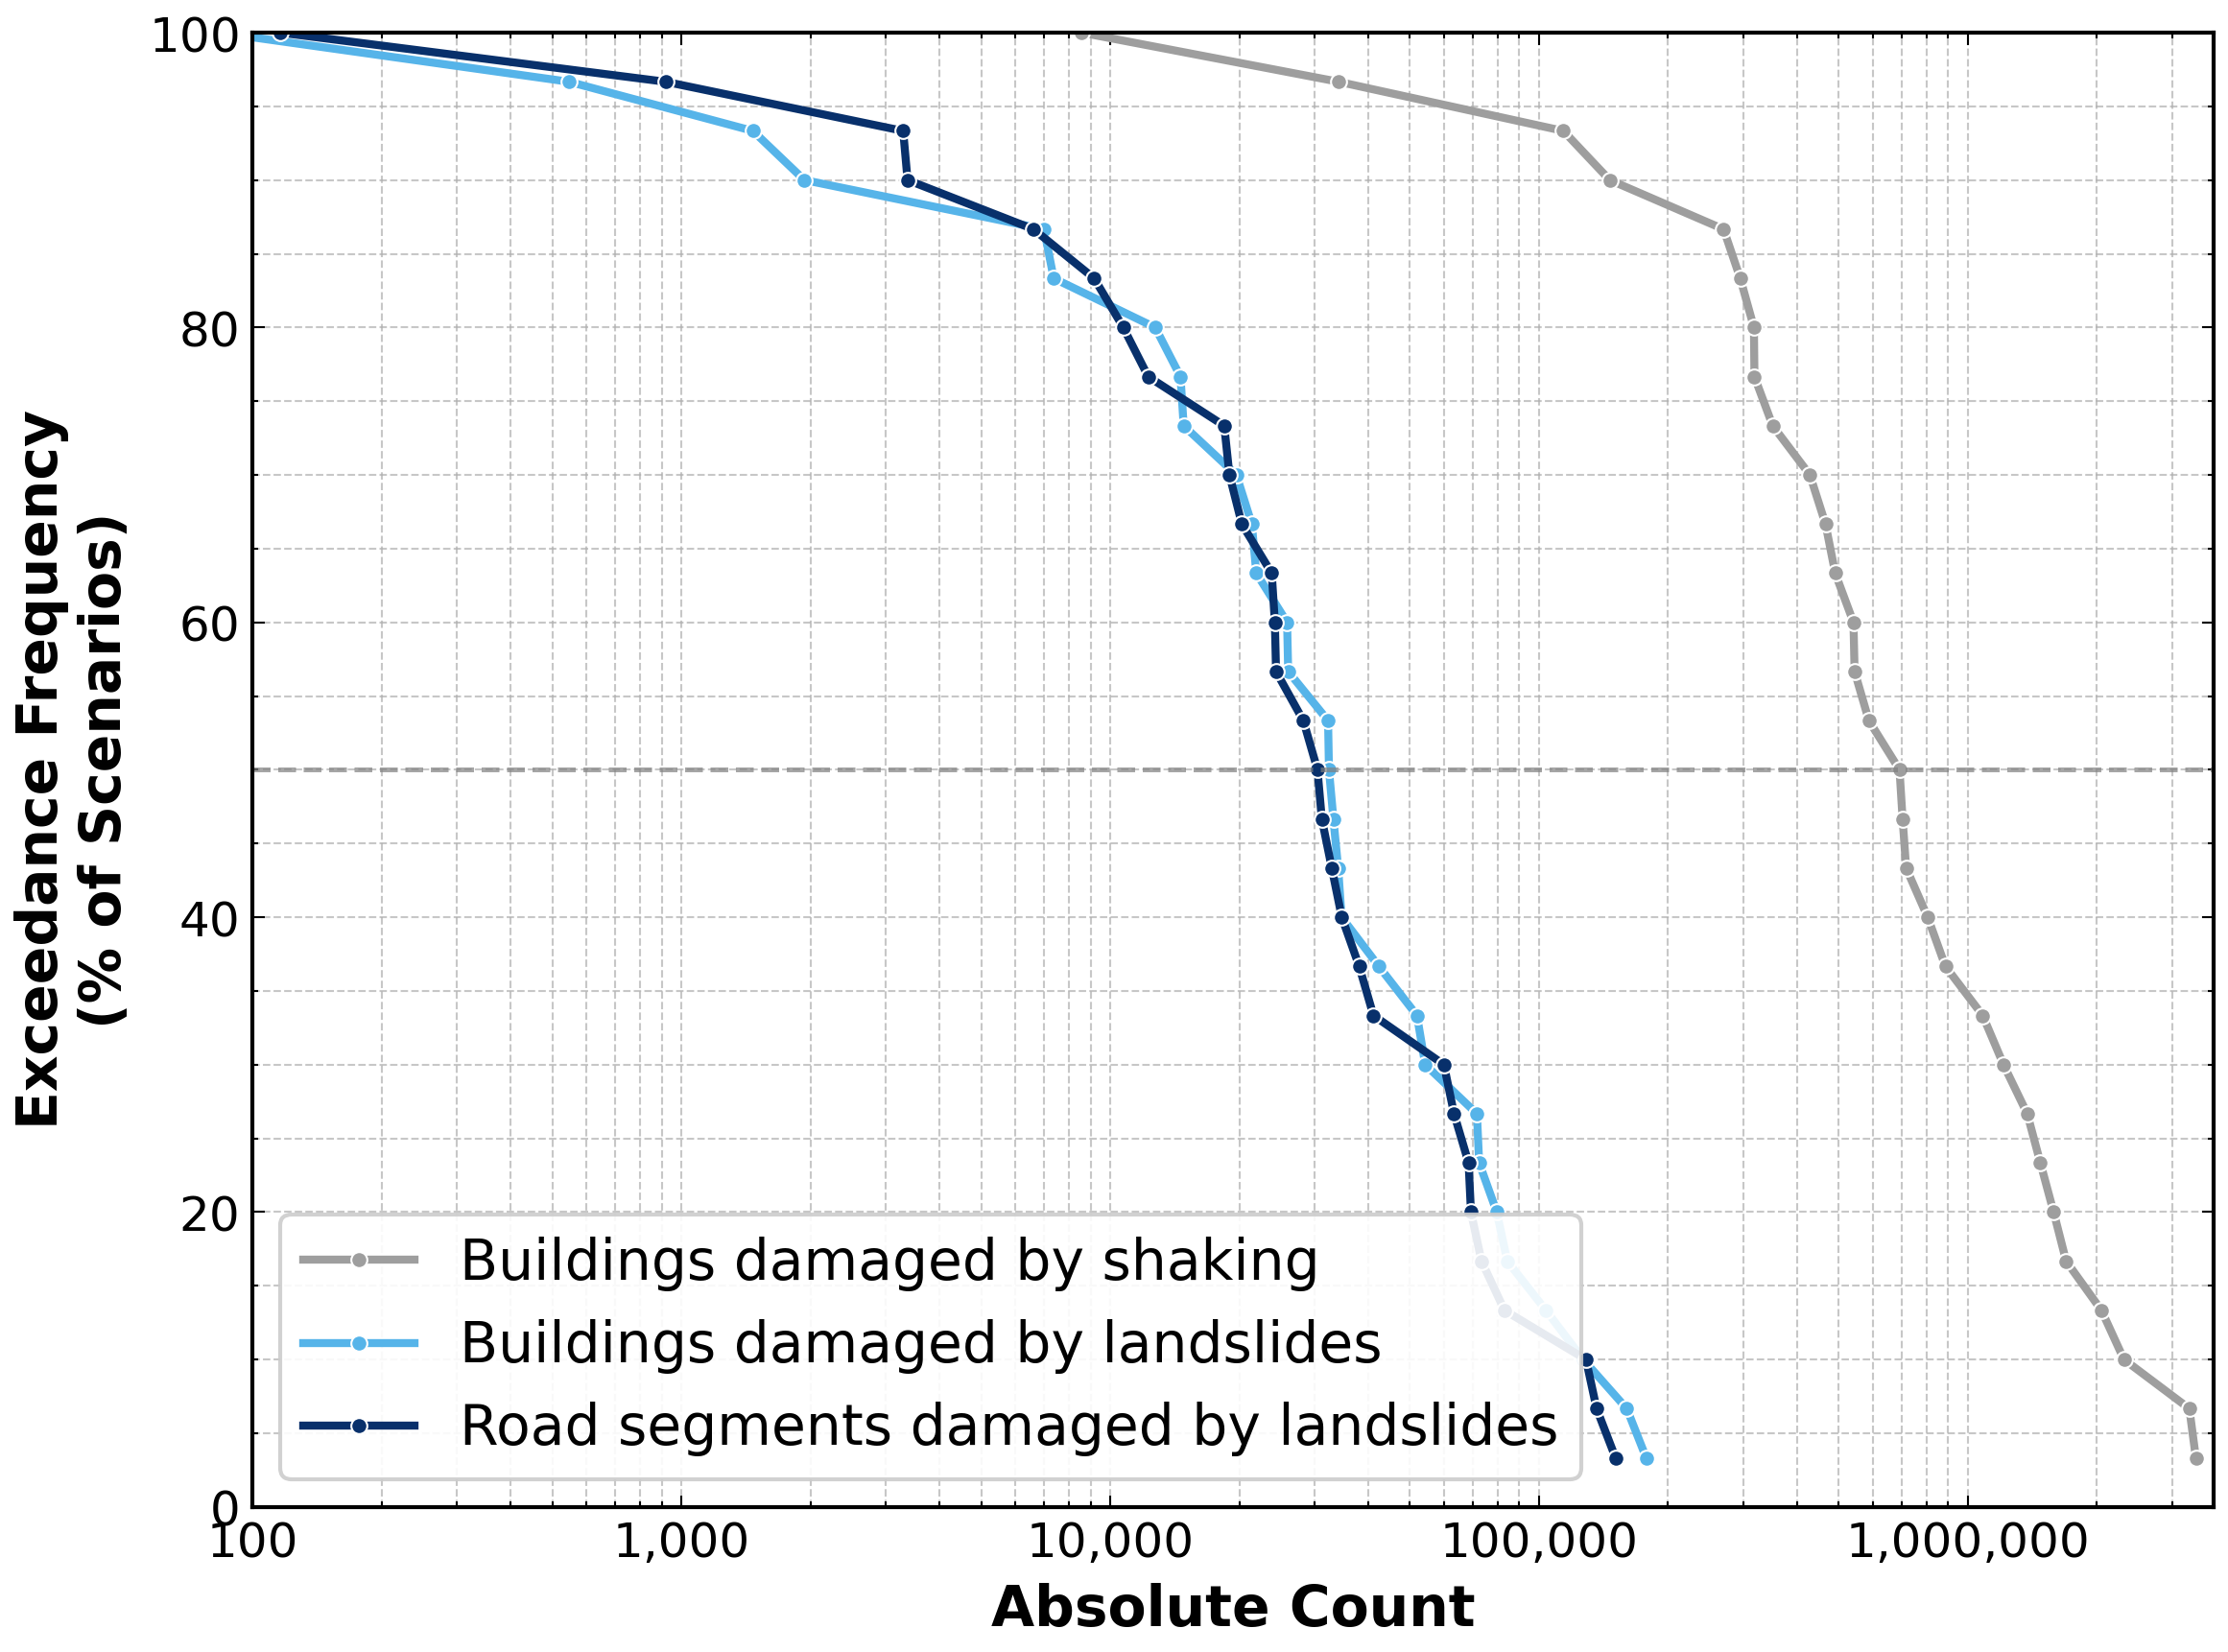
\includegraphics[width=0.75\linewidth]{./FIGURES/revised_v2/Fig2_exceedance_probability.png}
    \caption{Exceedance frequency of buildings damaged by earthquake shaking (grey), buildings damaged by coseismic landslides (light blue), and road segments damaged by coseismic landslides (dark blue) across the 30 scenario earthquakes. Exceedance frequency is the fraction of the 30 scenarios in which a given impact is equalled or exceeded. Horizontal dashed line shows the median impacts (50 percent exceedance frequency).}
    \label{fig:exceedance}
\end{figure}

Both the total number of modelled earthquake impacts and the ratio of damage by coseismic landslides to damage by shaking vary strongly across Nepal, depending upon both the shaking patterns in the scenario earthquakes and the underlying susceptibility to landsliding. Thus, while building damage from earthquake shaking represents the largest single category of damage in all of Nepal’s 77 districts, its proportional contribution to the total number of impacts is highly variable (Figure~\ref{fig:district_ratio}). If we consider the worst case of each impact type in each district, landslide impacts on buildings and roads are equivalent to between 1\% and 84\% of the number of buildings damaged by shaking. As expected, the ratio is lowest for districts located in the low-elevation, low-relief Terai region in southern Nepal; these areas are densely populated, with large numbers of buildings, but have low landslide susceptibility \citep{Kincey2021, Kincey2024}. Conversely, the highest ratios are found in the sparsely-populated mountain districts along the northern border of Nepal, including Darchula, Manang, Dolpa, and Mustang (see Figure~\ref{fig:study} for locations). More importantly for contingency planning, including landslide impacts changes the order in which districts would be prioritised. Ranking districts by the sum of the worst cases of the three impact types (total bar height in Figure~\ref{fig:district_ratio}A), rather than by worst-case shaking damage alone, moves several hill and mountain districts up the ranking, most notably Kalikot and Bajura (8 places each), Bajhang (7 places), and Baglung and Solukhumbu (6 places each). Conversely, Terai districts such as Mahottari and Parsa move down by up to 8 places. The ten most-affected districts are the same under both rankings, because their totals are dominated by shaking damage.

\begin{figure}[H]
    \centering
    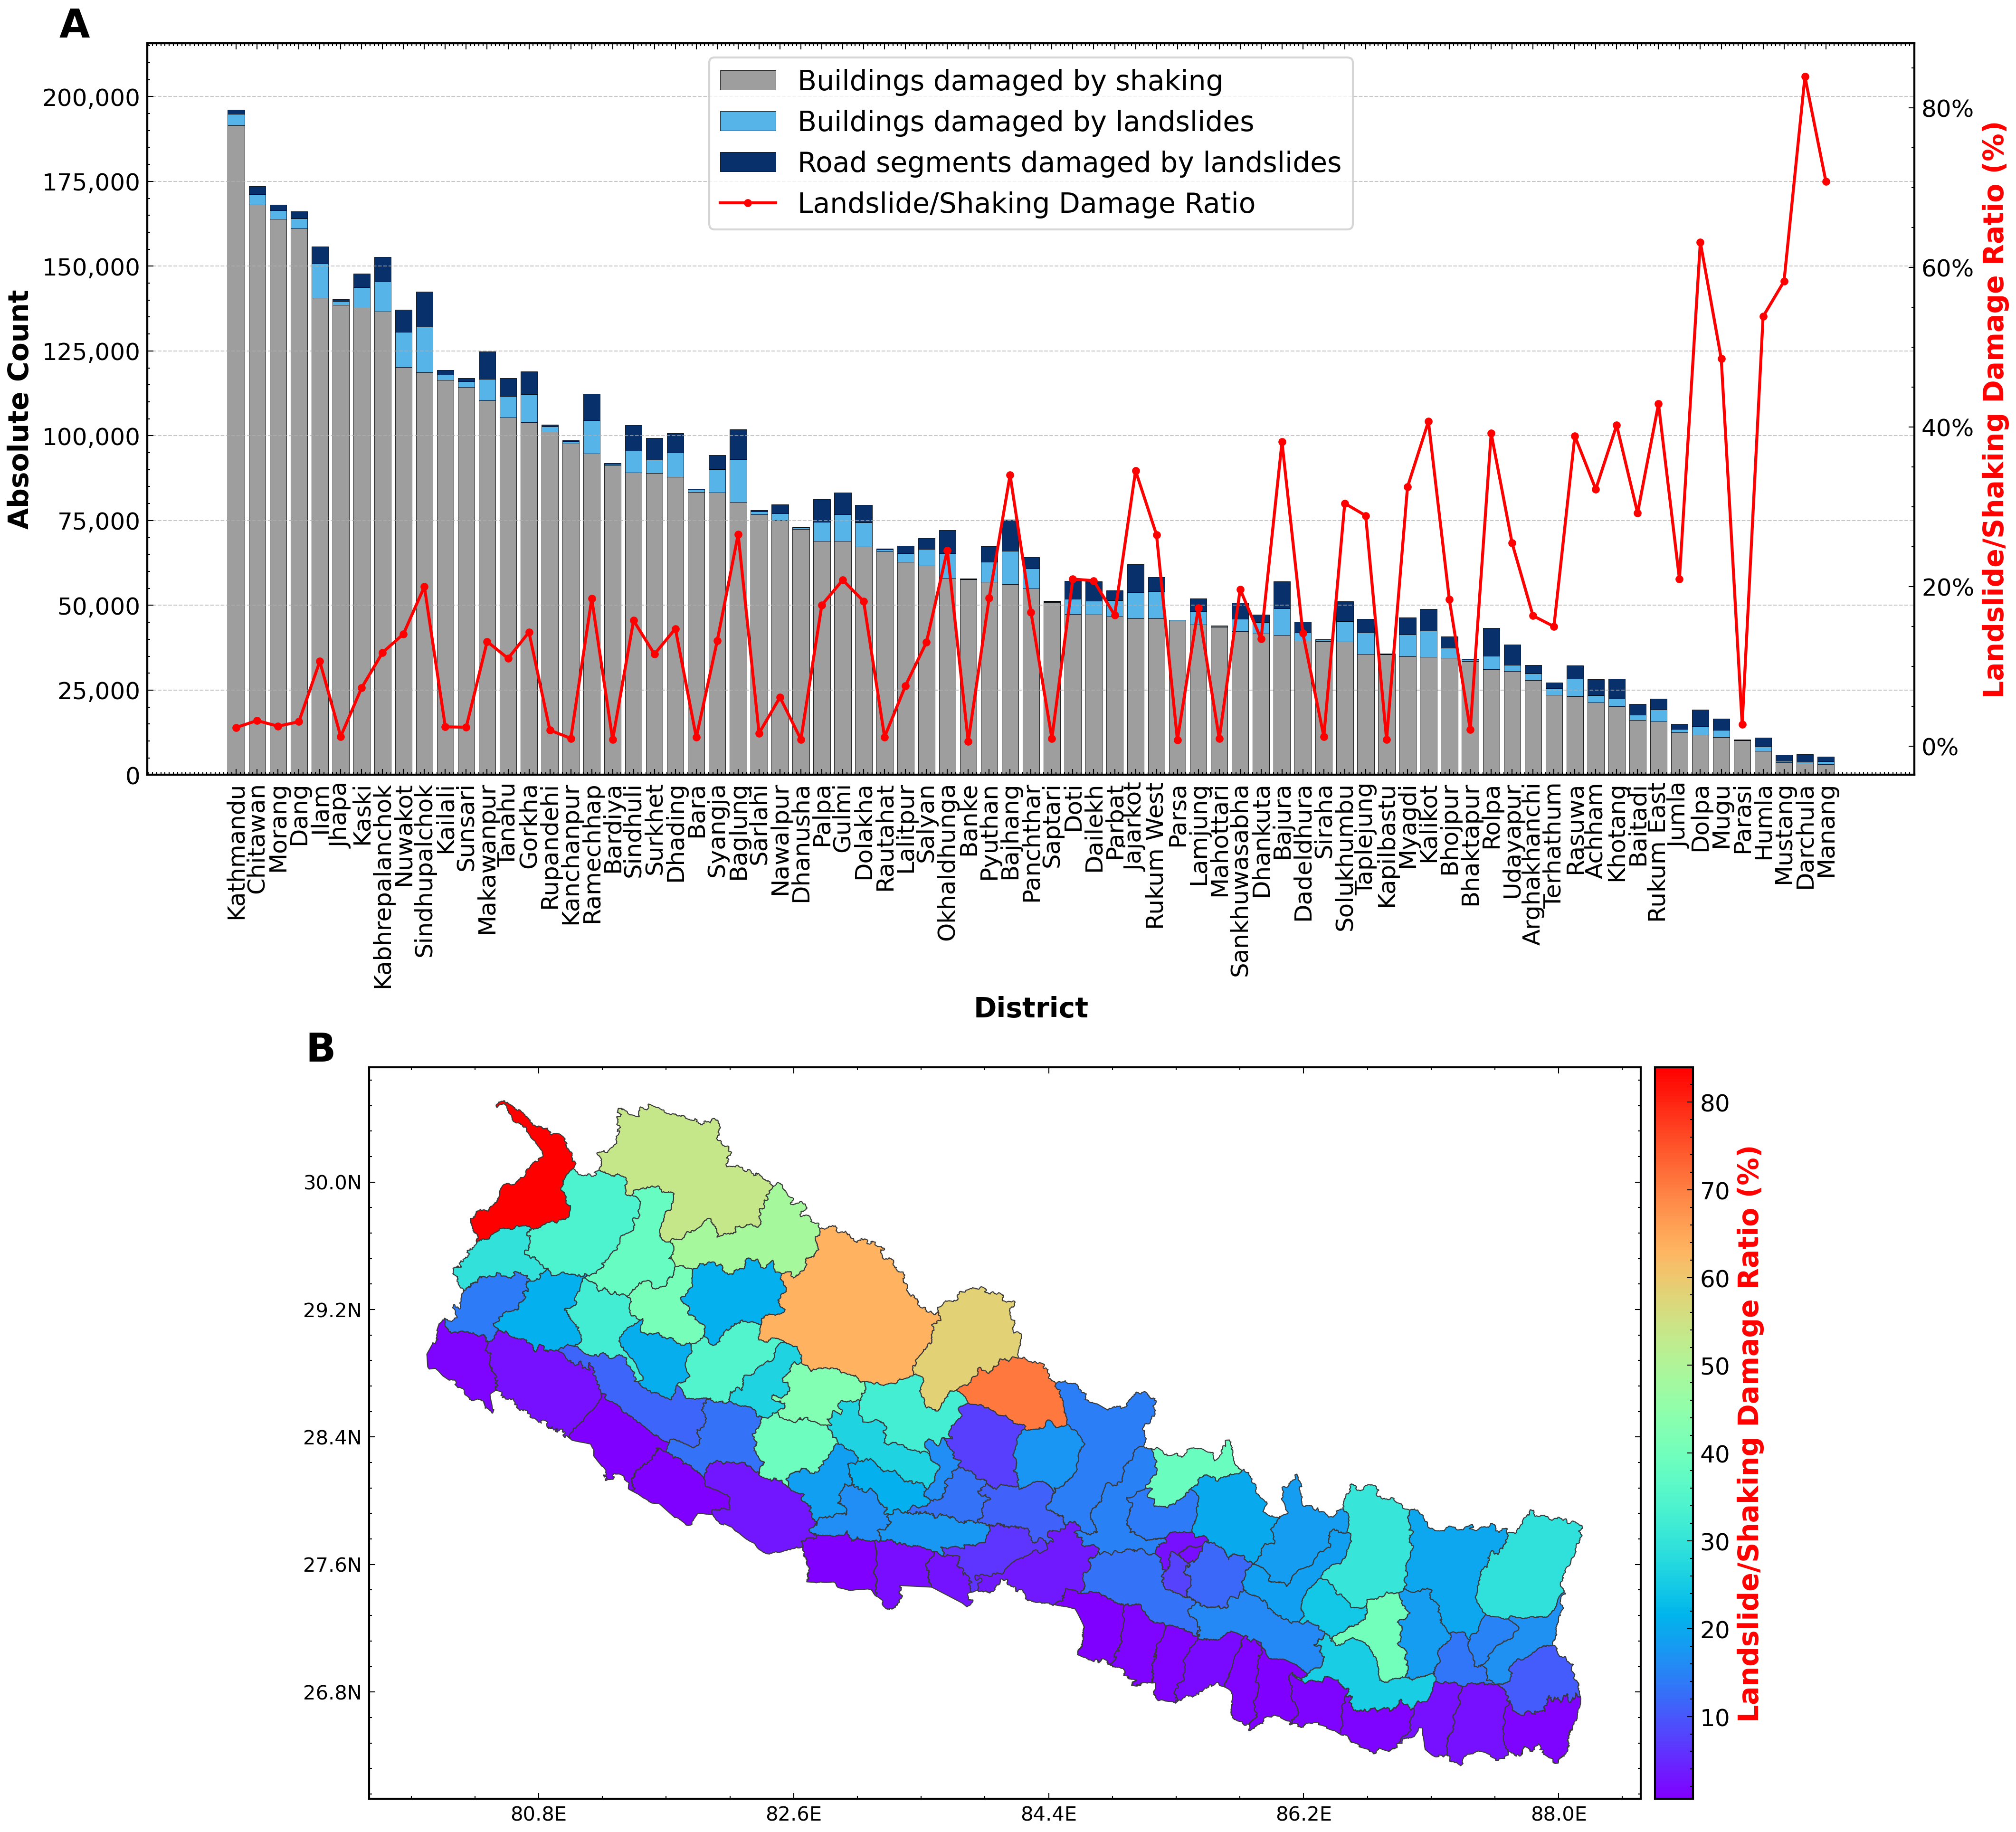
\includegraphics[width=1\linewidth]{./FIGURES/revised_v2/Fig3_district_impacts_ratio.png}
    \caption{A, district-wise plot of the range of buildings damaged by earthquake shaking (grey), buildings damaged by landslides (light blue), and road segments damaged by landslides (dark blue) across the 30 scenario earthquakes. In every district, the minimum across the 30 scenarios is zero for buildings damaged by shaking and less than one for both types of landslide impact, so the height of each bar segment shows the range of outcomes across the ensemble. Total bar height shows the sum of the worst cases of the three impact types in each district, which exceeds the largest single-scenario total by less than 1\% in every district. Bars are ordered by the highest maximum number of shaking-damaged buildings. The red line (right-hand axis) shows worst-case landslide impacts on buildings and roads as a percentage of the worst-case number of buildings damaged by shaking. B, district-wide map of worst-case landslide impacts on buildings and roads as a percentage of the worst-case number of buildings damaged by shaking. Note that the highest values are found in sparsely-populated mountain districts in northern Nepal.}
    \label{fig:district_ratio}
\end{figure}

Exceedance frequency curves by district show that between 33\% and 63\% of scenarios result in an expected number of at least one building per district completely damaged by shaking (Figure~\ref{fig:district_exceedance}A). In comparison, 30\% to 87\% of scenarios result in an expected number of at least one building damaged by landslides (Figure~\ref{fig:district_exceedance}B), and 27\% to 77\% with an expected number of at least one road segment damaged by landslides (Figure~\ref{fig:district_exceedance}C). However, the median number of landslide-induced impacts is generally below 10 per district, confirming that landslide impacts are smaller in number than shaking impacts but still widespread across scenarios. As expected, the exceedance frequency curves show distinct physiographic variations \citep{upreti_physiography_2001}. Districts in the Terai lowlands in southern Nepal have high exceedance frequencies for shaking damage but consistently low frequencies for landslide impacts, reflecting their high building exposure but low relief and limited slope instability. In contrast, hill and middle mountain districts have more variable exceedance patterns, with several districts showing higher exceedance frequencies for landslide impacts than for shaking damage, particularly for road damage. High mountain districts have the most variable patterns, with some showing very low exceedance frequencies due to sparse infrastructure, while others have disproportionately high landslide exceedance frequencies relative to their larger shaking exposure. These physiographic trends highlight how topographic setting fundamentally controls the relative importance of different hazard components across Nepal's diverse landscape.

\begin{figure}[H]
    \centering
    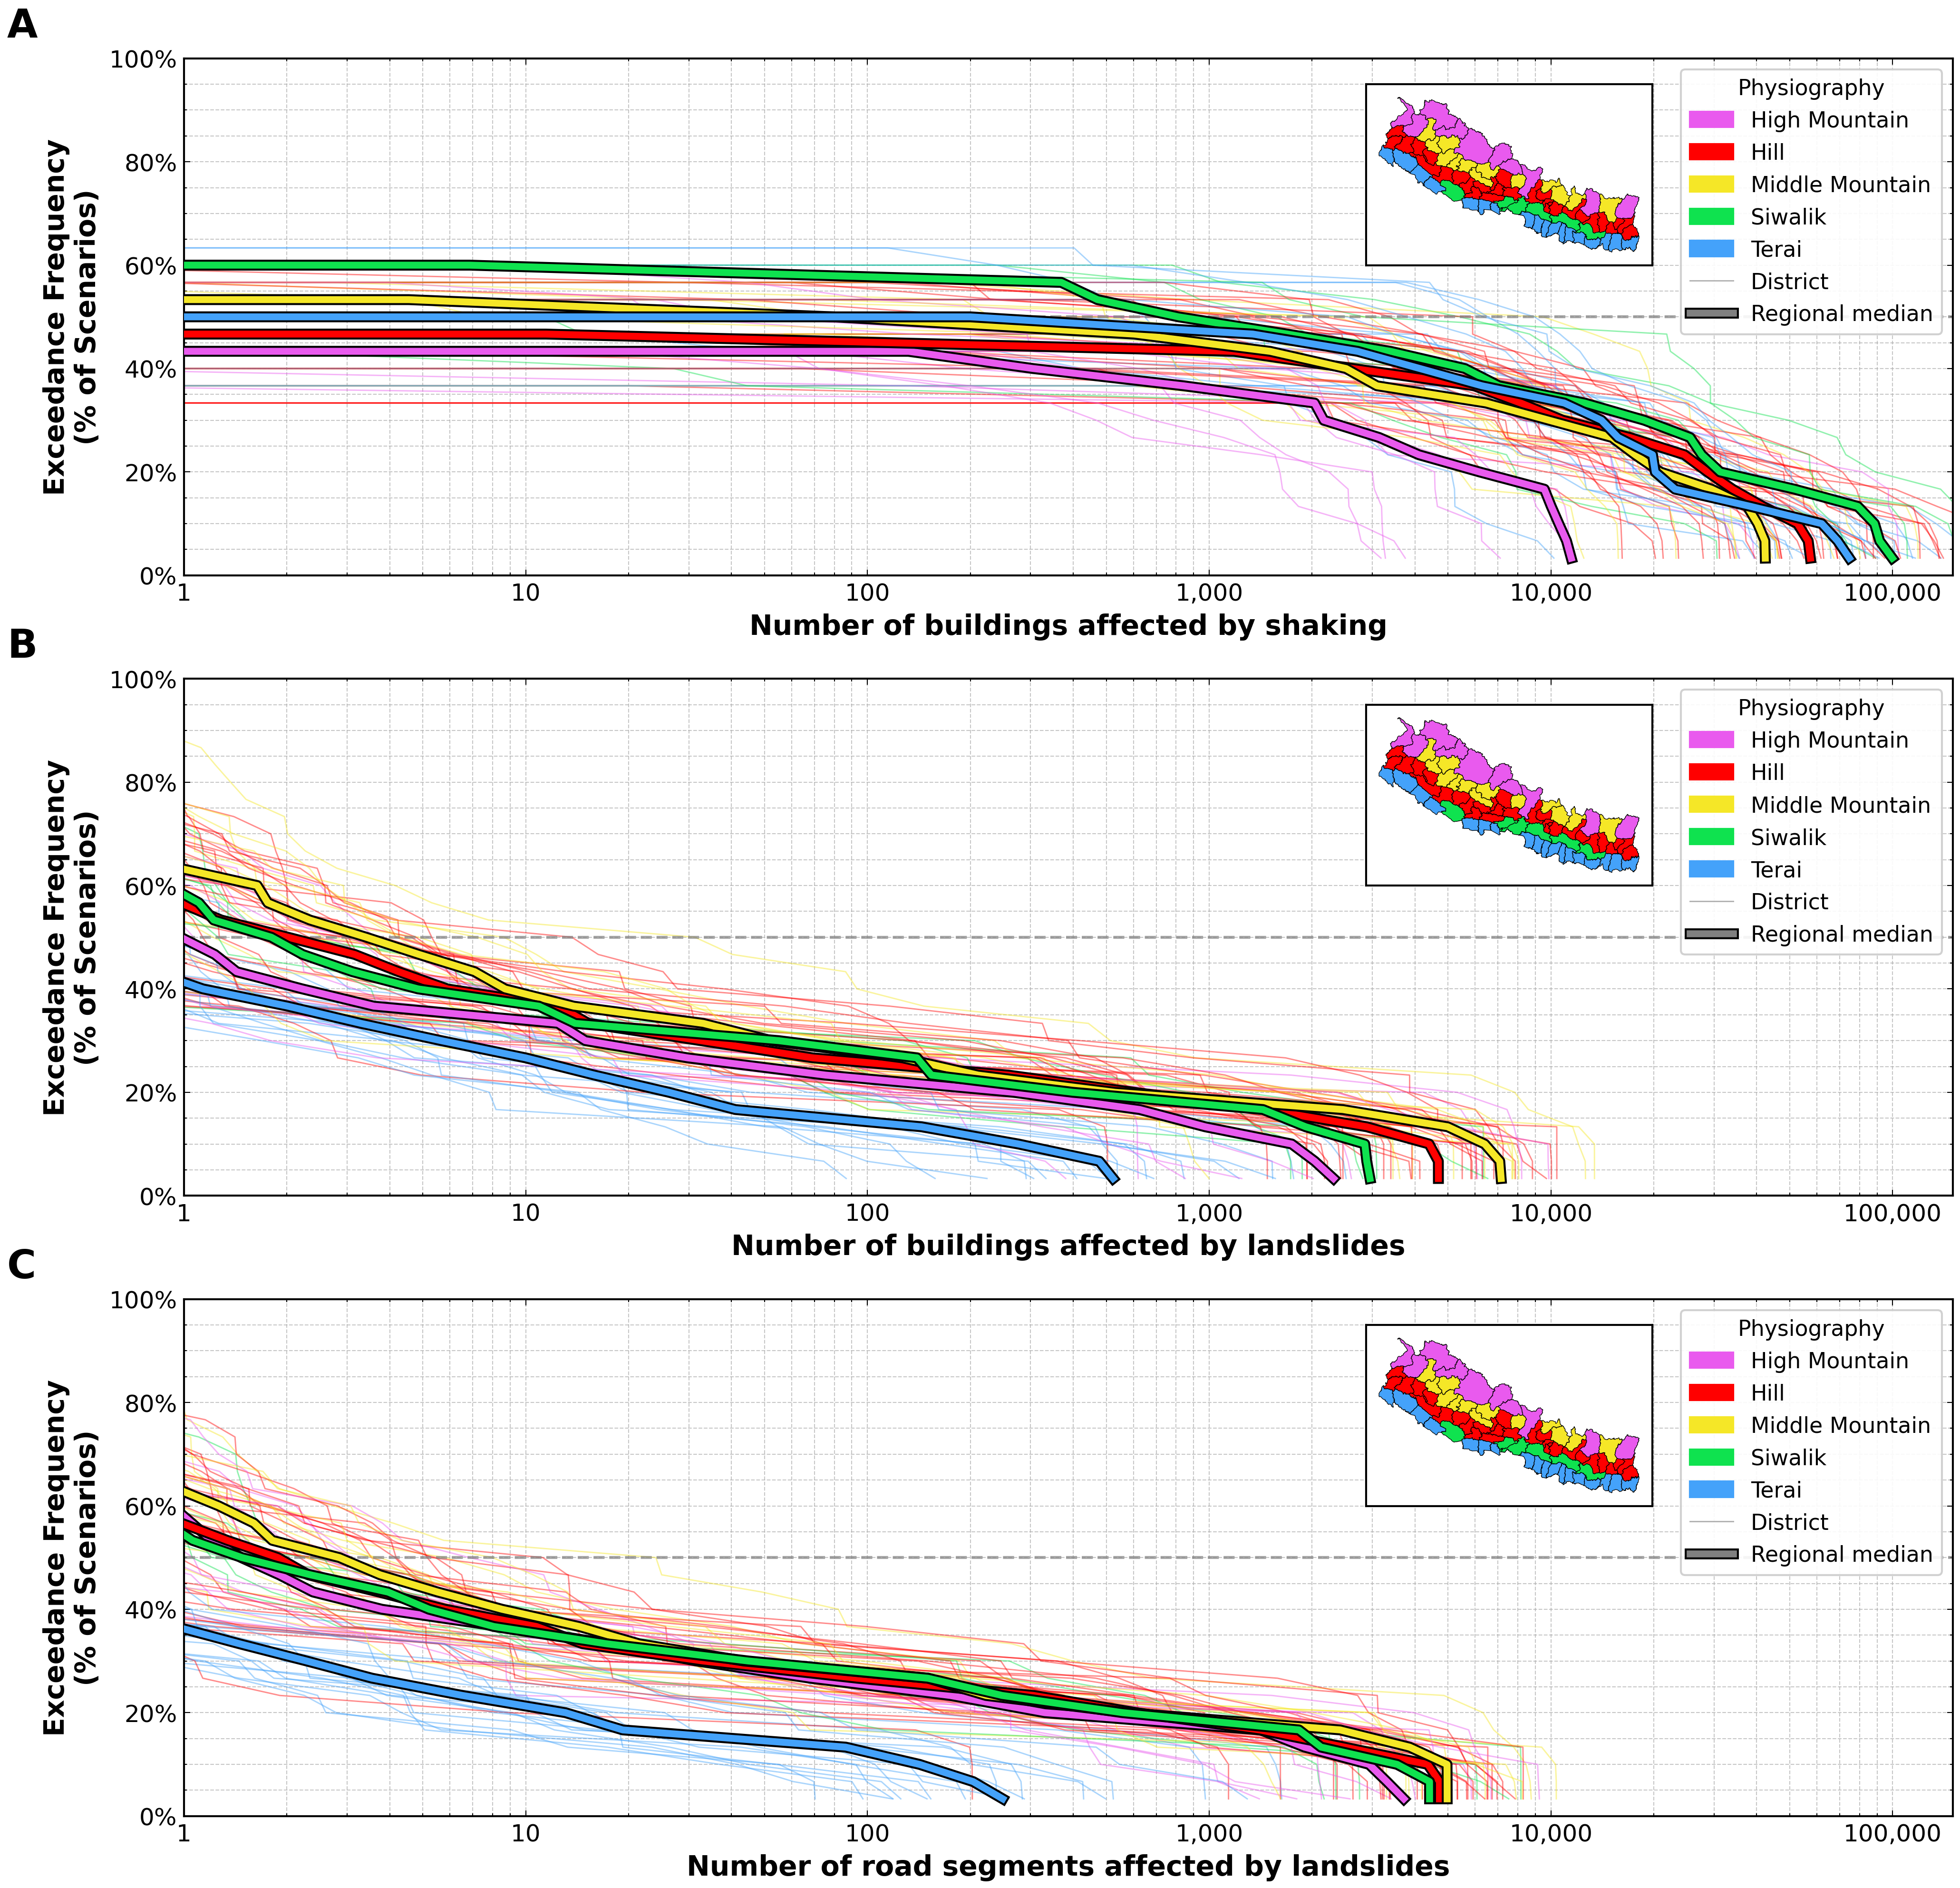
\includegraphics[width=1\linewidth]{./FIGURES/revised_v2/Fig4_district_exceedance_curves.png}
    \caption{A, exceedance frequency of buildings damaged by earthquake shaking in each of the 77 districts in Nepal across the 30 scenario earthquakes. Each thin line shows an exceedance curve for a single district, coloured by the physiographic setting of the district. Thick lines show the median curve of each physiographic region, that is, the median across the districts of the region of the number of damaged assets at each exceedance frequency. Median impacts for each district across the ensemble are shown by where the curves intersect the 50\% line (dashed horizontal line), while worst-case impacts are shown by the intersection with the x axis. B, exceedance frequency of buildings damaged by landslides in each district. C, exceedance frequency of road segments damaged by landslides in each district.}
    \label{fig:district_exceedance}
\end{figure}

Districts with the largest expected numbers of damaged buildings, both in the median and the worst-case scenarios, are concentrated in the more populated southern and central areas of the country (Figure~\ref{fig:worst_case_maps}A), highlighting not only building density and population distribution but also patterns of infrastructure vulnerability (Figure~\ref{fig:S3}). Districts in the more remote and more sparsely-populated northwest have relatively low total numbers of shaking-damaged buildings, even in the worst case. In contrast, while the absolute numbers of expected landslide impacts are lower, the largest number of landslide impacts are concentrated in hill and mountain districts across Nepal (Figure~\ref{fig:worst_case_maps}C, E). Road impacts from landslides are widely distributed through the hill and mountain districts, with particular hotspots in Sindhupalchok, Baglung, Rolpa, Bajura, and Bajhang (Figure~\ref{fig:worst_case_maps}E). These areas should be considered at the highest risk of disruption to the road network after a future large earthquake. Building impacts from landslides are more focused on the hill and middle mountain districts, likely because of the concentration of population in those areas (Figure~\ref{fig:worst_case_maps}C). Not surprisingly, expected landslide impacts are lower in the flat-lying southern districts of the Terai, along the border with India (Figure~\ref{fig:worst_case_maps}D, F). The dominance of shaking impacts over landslide impacts means that their sum, which we take as the worst-case expected total number of earthquake impacts (the sum of the worst cases of each impact type), mirrors the distribution of shaking damage, although numbers of impacts are notably higher in the hill districts in particular (compare Figure~\ref{fig:worst_case_maps}C and A). As shown above, these additional impacts are large enough to move several hill and mountain districts up the ranking of total impacts, relative to a ranking based on shaking damage alone, so that focusing on shaking alone would give a different priority profile for contingency planning.

\begin{figure}[H]
    \centering
    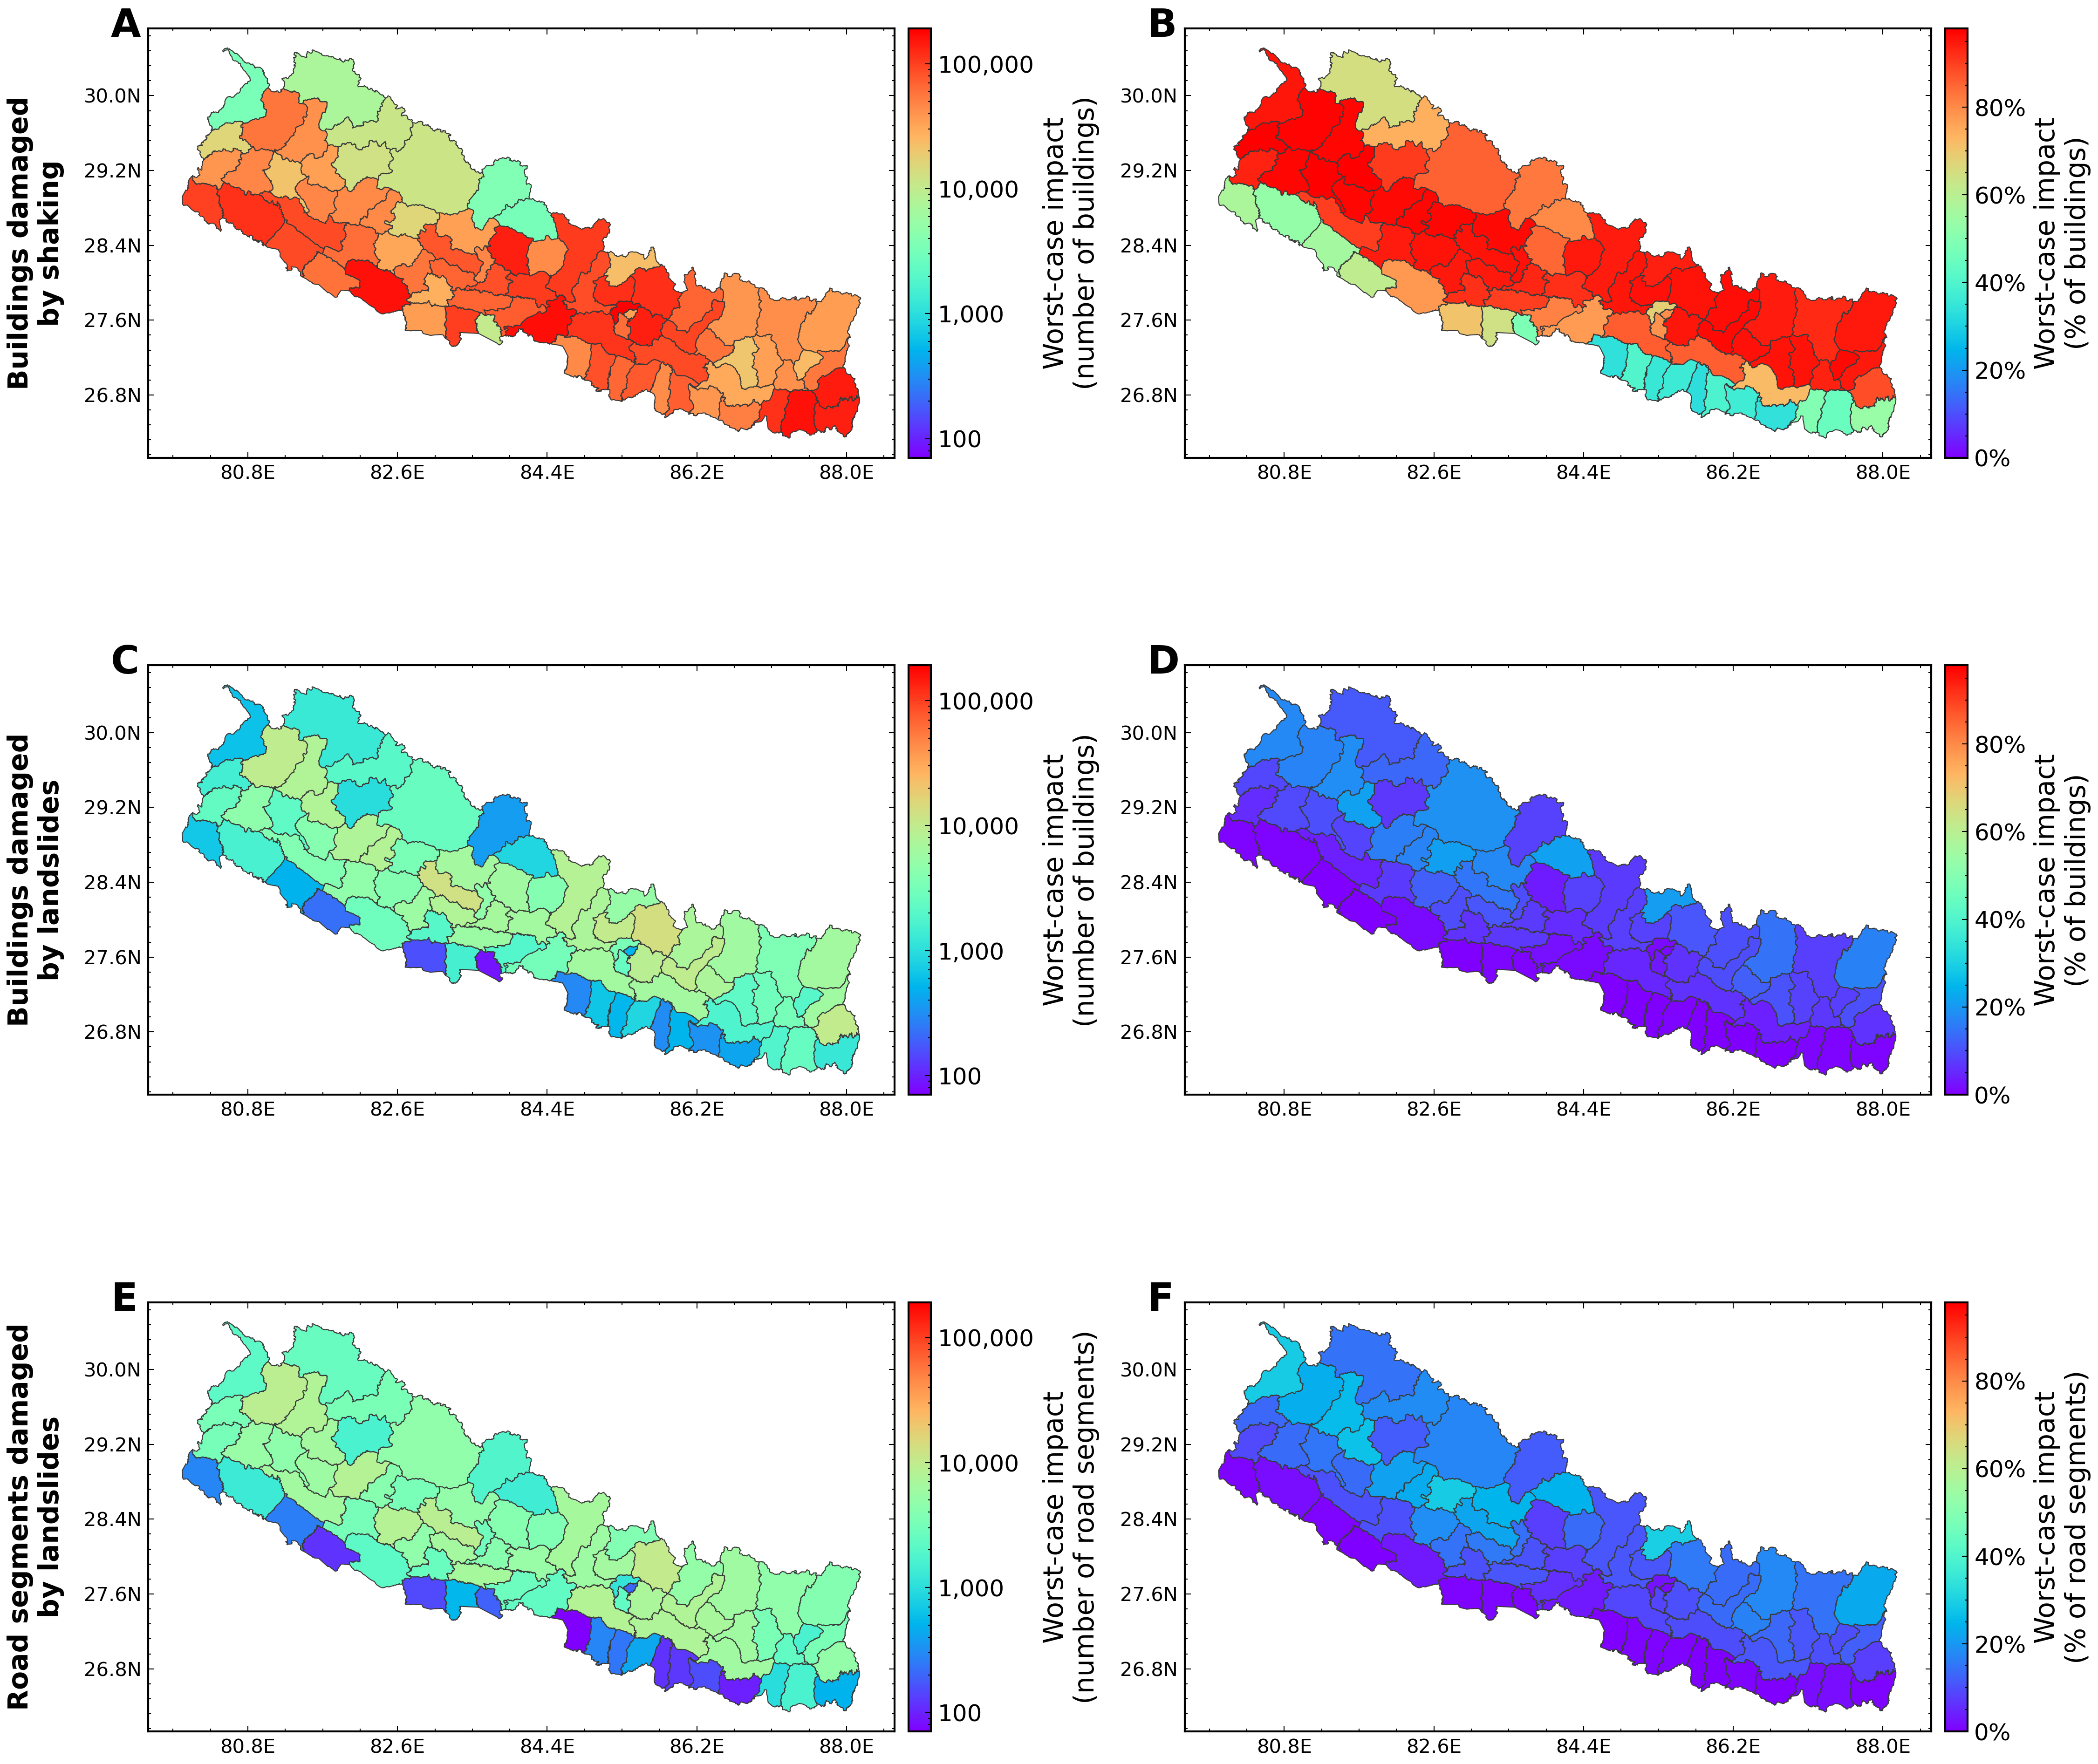
\includegraphics[width=1\textwidth]{./FIGURES/revised_v2/Fig5_worst_case_absolute_proportional.png}
    \caption{Maps of earthquake impacts by district. Left column: worst-case absolute numbers of (A) buildings damaged by shaking, (C) buildings damaged by landslides, and (E) road segments damaged by landslides. Right column: worst-case proportion (in percent) of (B) buildings damaged by shaking, (D) buildings damaged by landslides, and (F) road segments damaged by landslides. Proportions are relative to the total number of buildings (B, D) or road segments (F) in each district, so the three panels are independent of one another and are not expected to sum to 100\%.}
    \label{fig:worst_case_maps}
\end{figure}

District-level variability is further explored in Figure~\ref{fig:standard_deviation}, which maps the standard deviation of impacts for each district. In absolute terms, the standard deviation is highest for shaking-induced building damage (Figure~\ref{fig:standard_deviation}A), reflecting the large number of buildings exposed to shaking. However, the standard deviations for landslide-related impacts (Figure~\ref{fig:standard_deviation}C, E) reveal distinct hotspots in the hill and mountain districts. This indicates, as expected, that while shaking damage is widespread, severe landslide impacts are more scenario-dependent, occurring at high intensities only under specific earthquake conditions.


\begin{figure}[H]
    \centering
    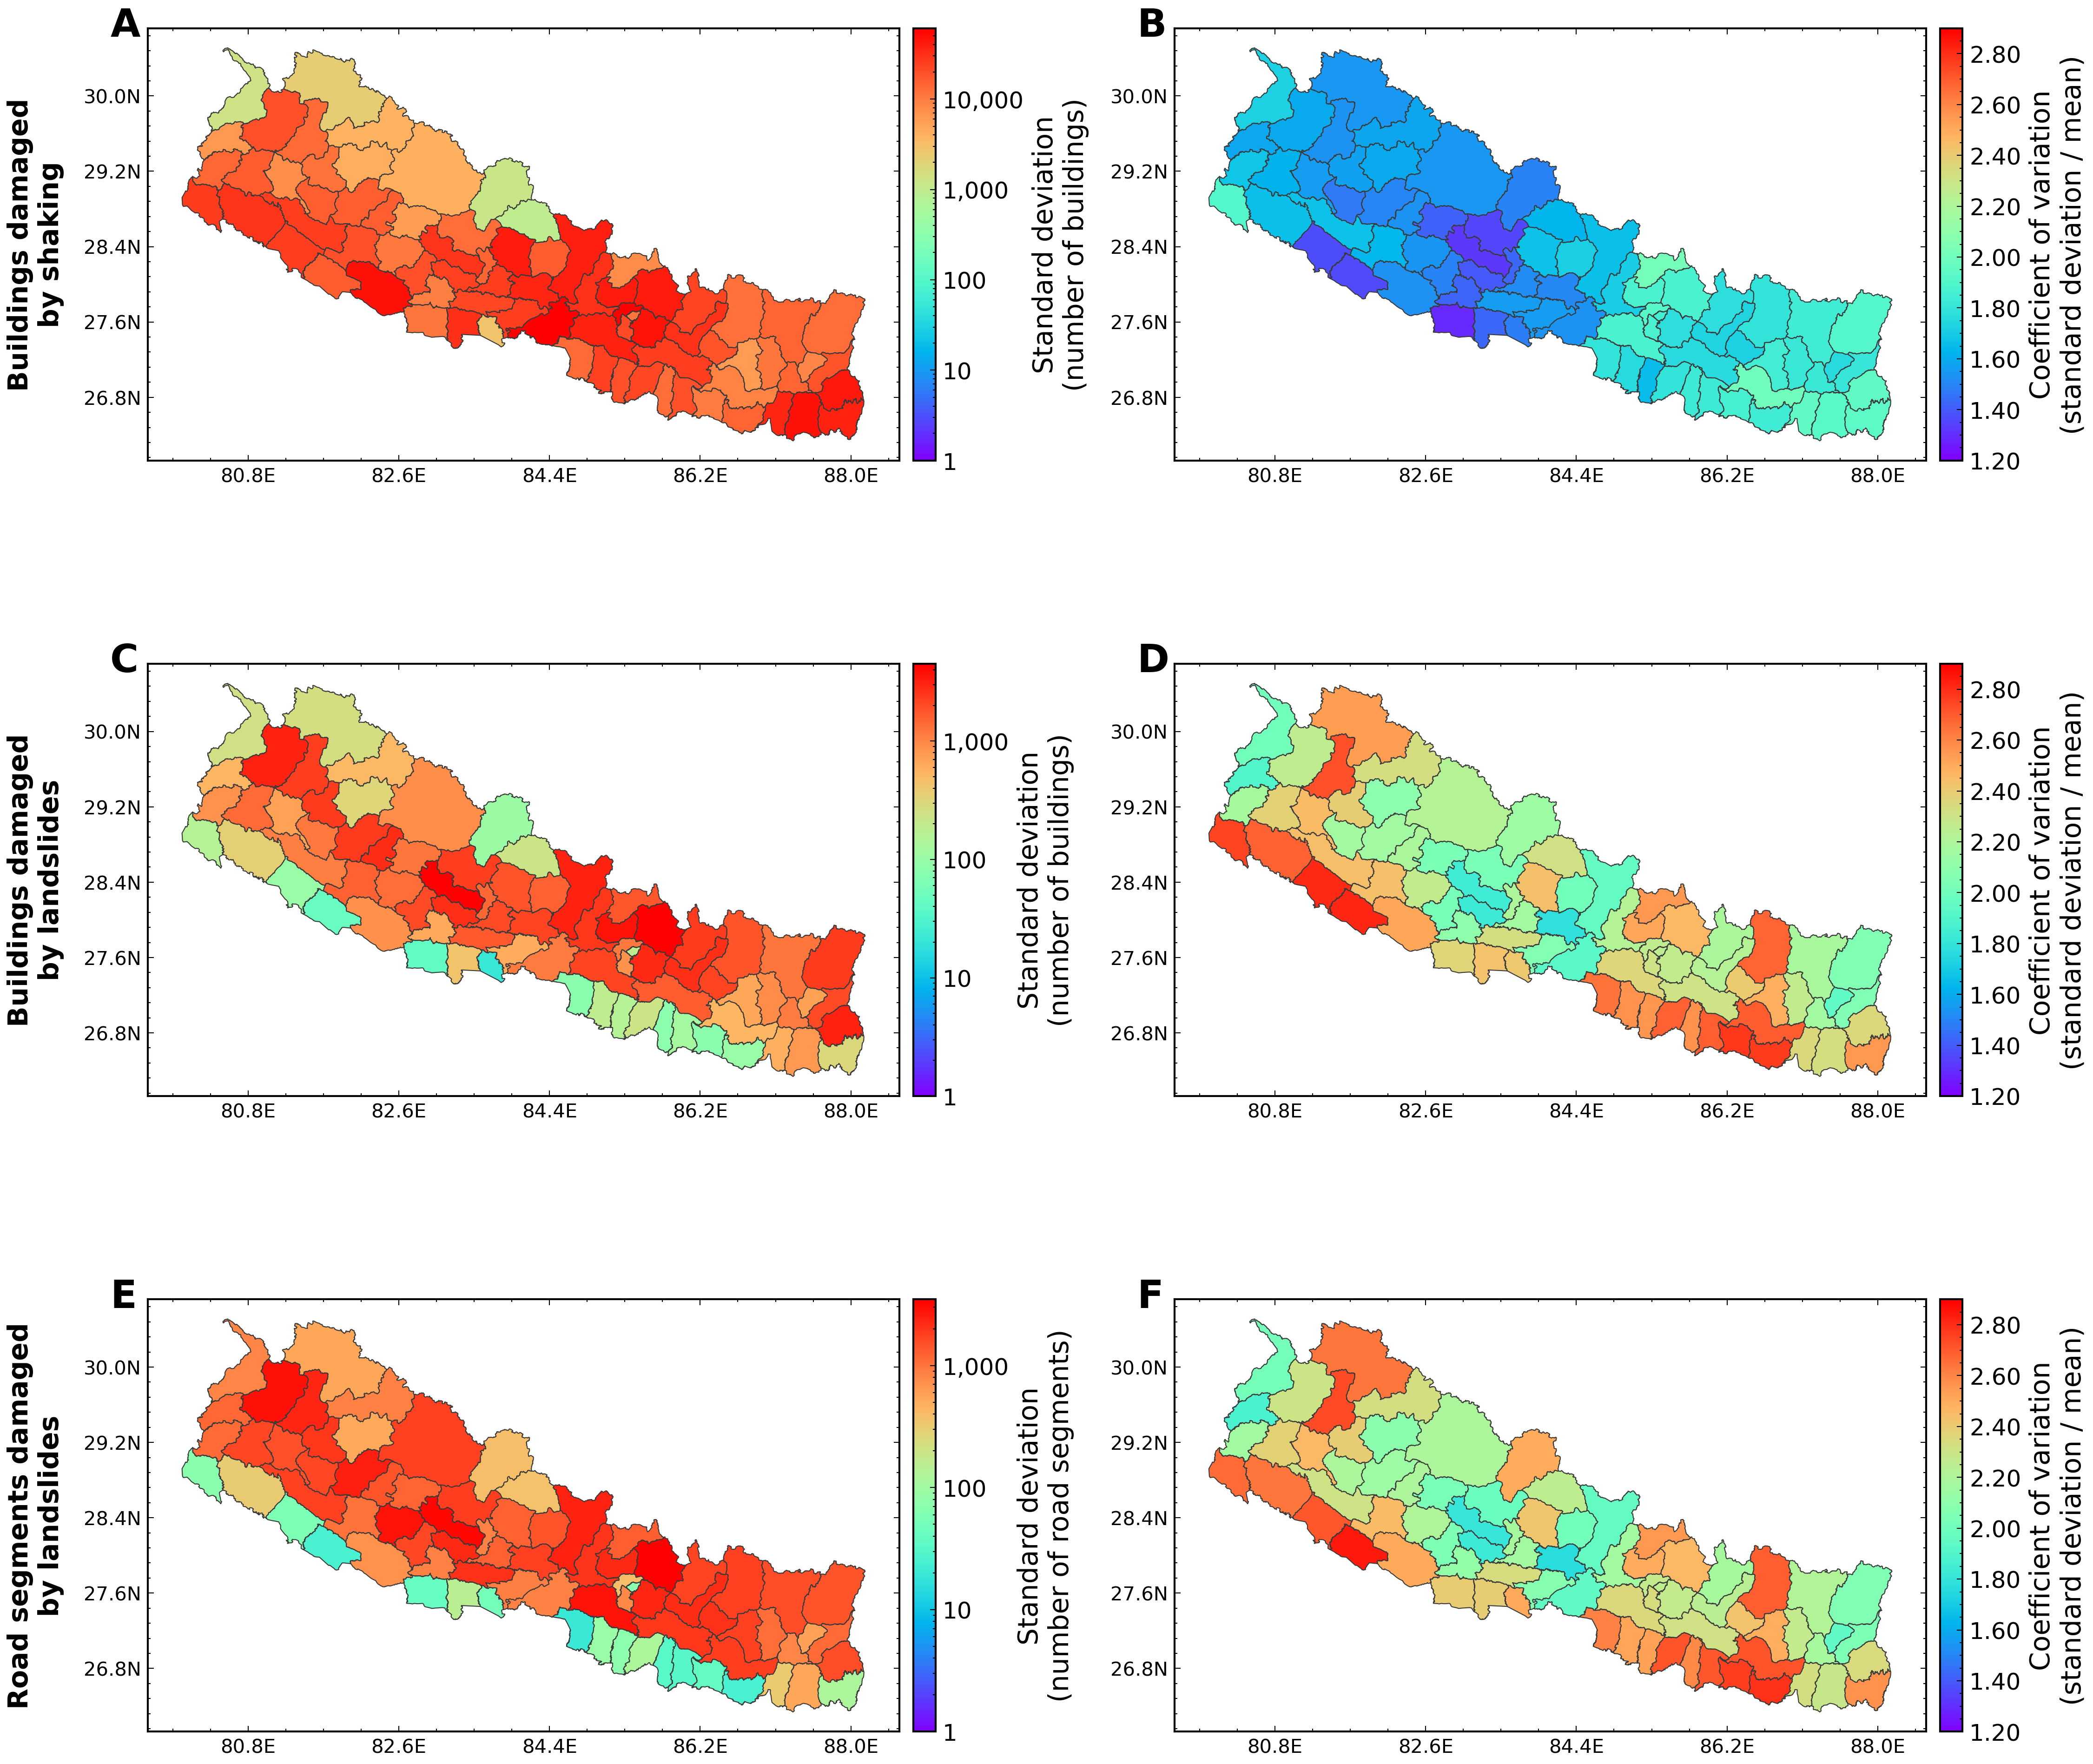
\includegraphics[width=1\linewidth]{./FIGURES/revised_v2/Fig6_standard_deviation.png}
    \caption{Variability of impacts across the 30 scenarios. Left column: standard deviation (absolute spread) of (A) buildings damaged by shaking, (C) buildings damaged by landslides, and (E) road segments damaged by landslides. Right column: coefficient of variation (standard deviation divided by the mean; relative spread) of the same impacts (B, D, F). The standard deviation scales with the number of exposed assets, whereas the coefficient of variation does not; high coefficients of variation indicate districts where impacts occur in only a few scenarios relative to their typical level. Note that the range of standard deviations is approximately ten times greater in panel A than in panels C and E. The three coefficient-of-variation panels share the same colour scale.}
    \label{fig:standard_deviation}
\end{figure}

\subsection{Remoteness, impacts, and risk scores}
\label{sec:results_remoteness}

The index of remoteness from health facilities (Figure~\ref{fig:remoteness}A) shows values ranging from near 0 in southern districts to 1 in Manang, followed by Dolpa (0.65); other northern and northwestern districts, such as Humla, Darchula and Kalikot, have values of 0.3--0.4. Comparing remoteness from health facilities with remoteness from the district headquarters (Figure~\ref{fig:remoteness}B) shows that remoteness values from district headquarters are higher than those from health facilities in 91\% of districts. The largest differences are found in Darchula, Bajhang, Dolpa, Jajarkot and Humla, while Manang is the only district that lies clearly above the 1:1 line.

\begin{figure}[H]
    \centering
    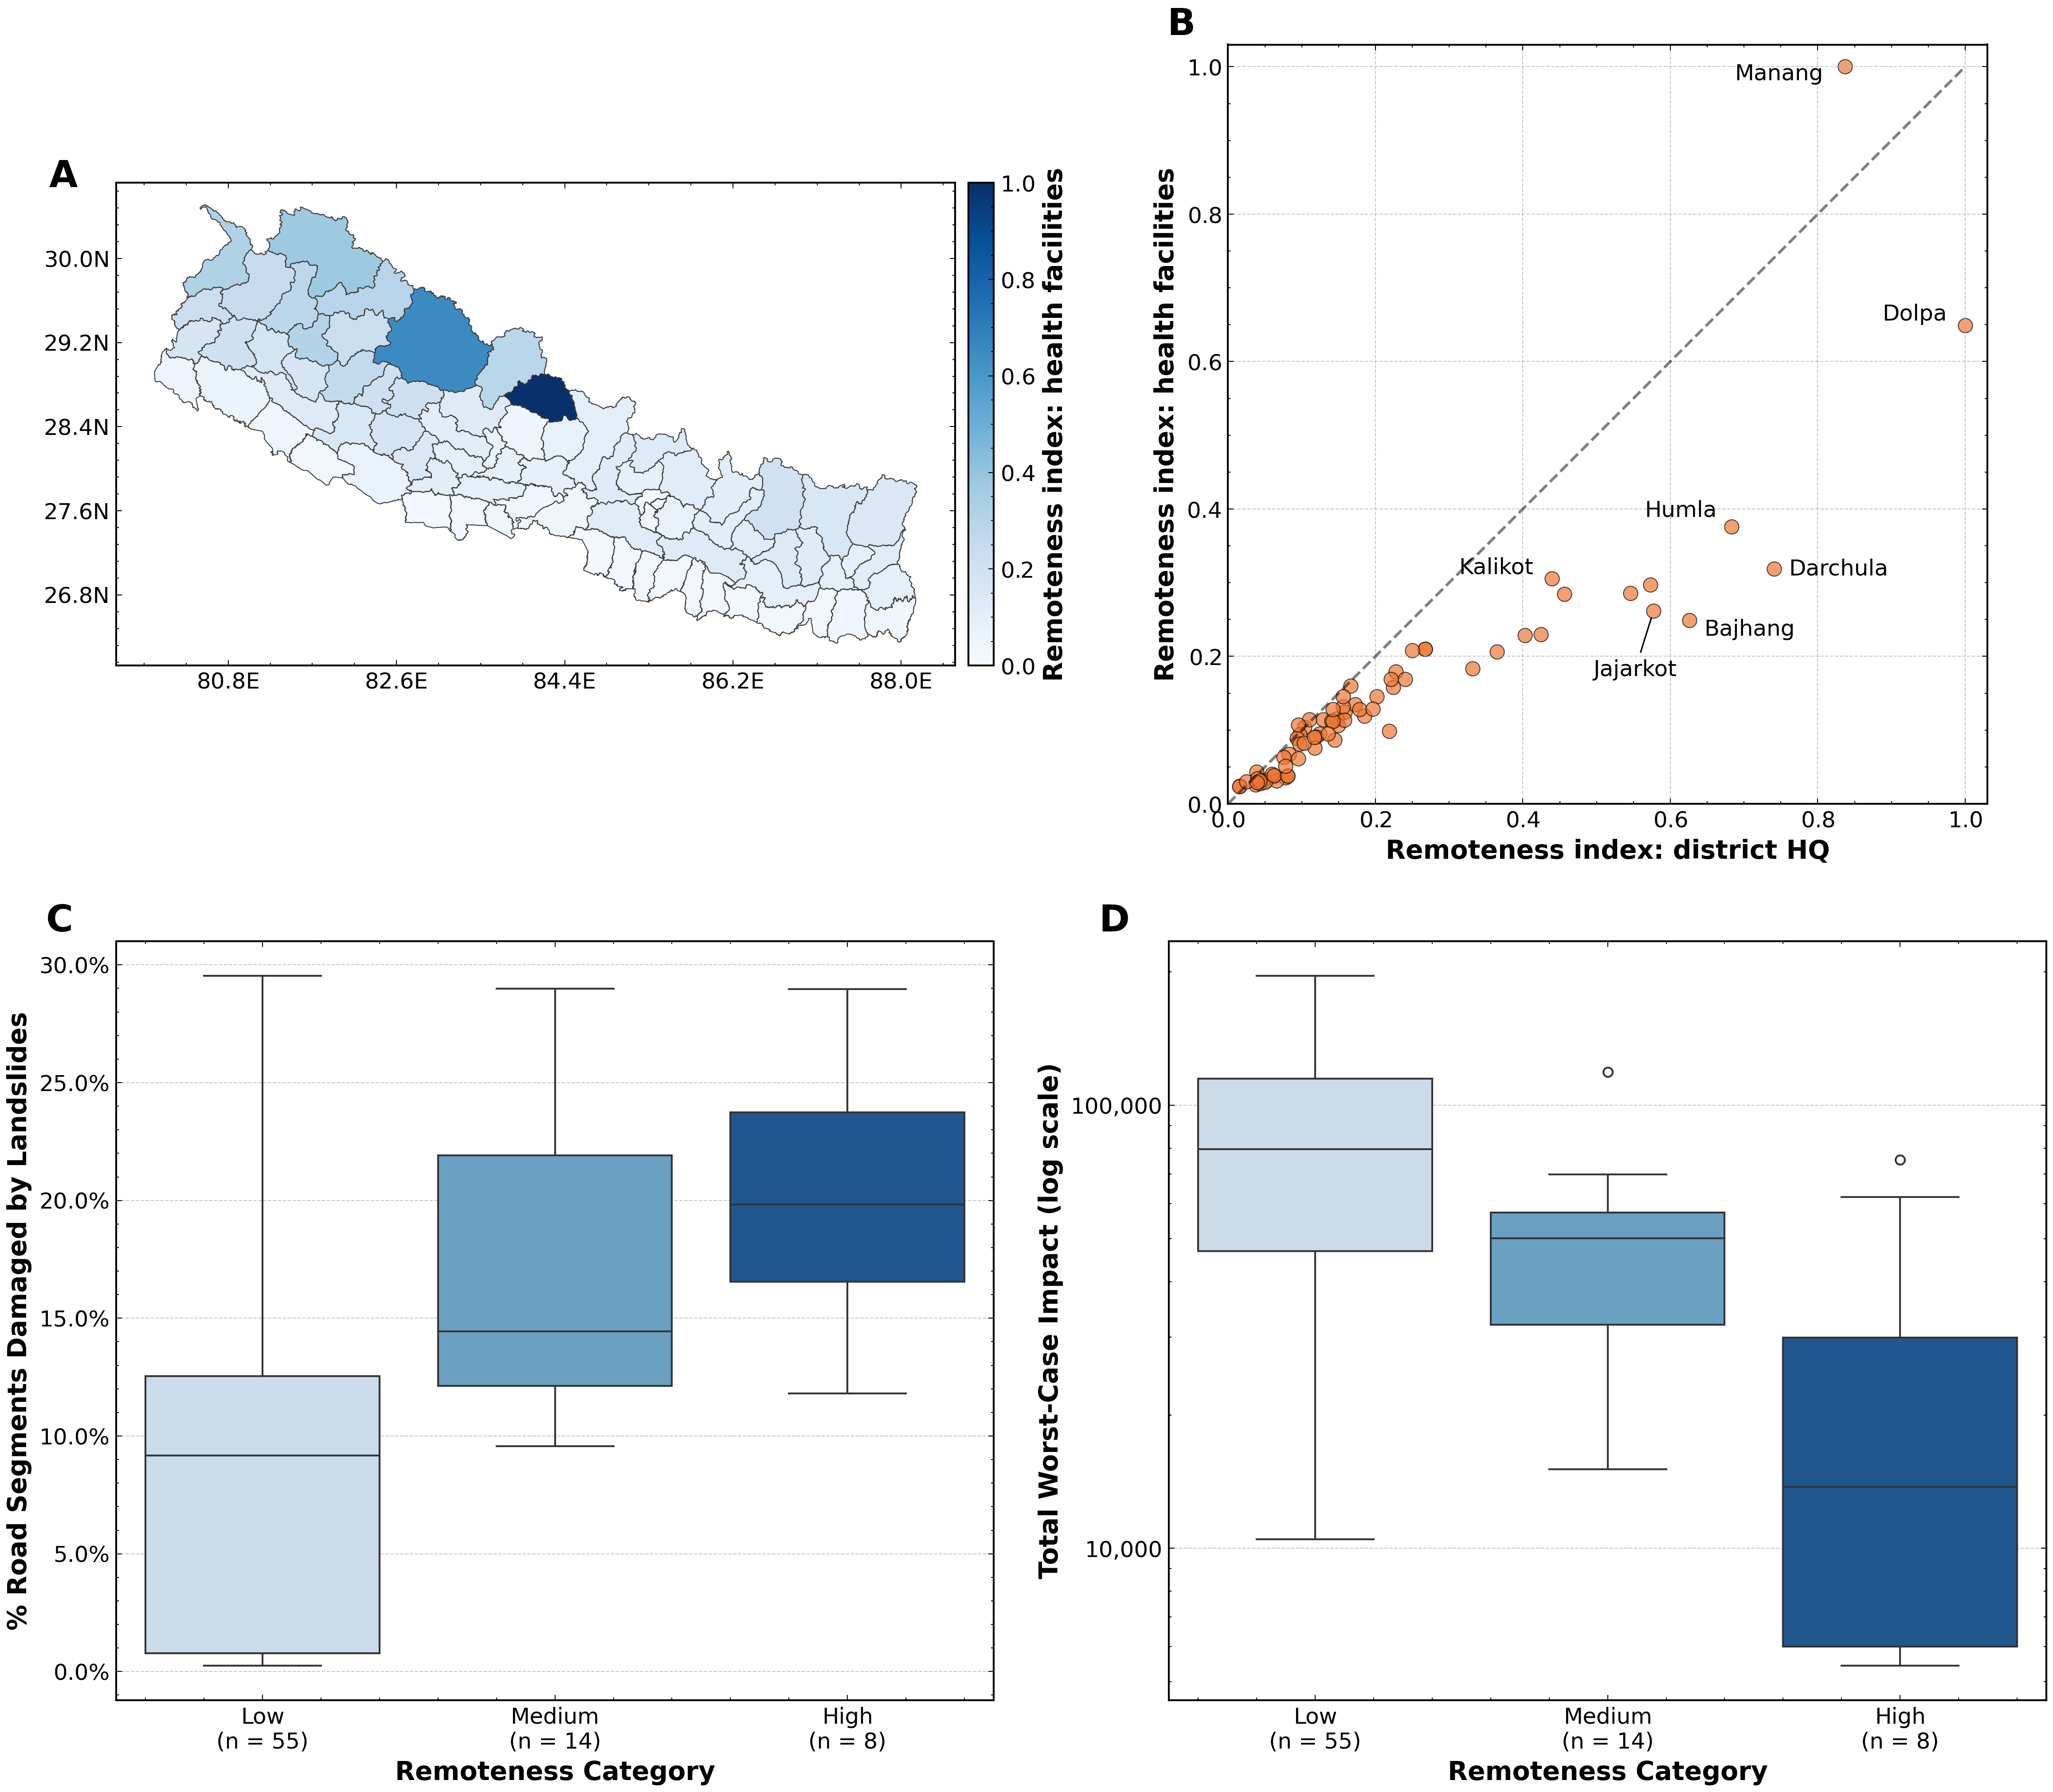
\includegraphics[width=1\linewidth]{./FIGURES/revised_v2/Fig7_remoteness_analysis.png}
    \caption{Combined analysis of remoteness and vulnerability. A, map of remoteness index from health facilities. B, comparison of remoteness from district headquarters (x-axis) against remoteness from health facilities (y-axis). The dashed line represents a 1:1 relationship; labelled districts are discussed in the text. C, box plots showing the percentage of road segments damaged by landslides across the three remoteness categories (low, medium, high); the number of districts in each category is given below each box. D, box plots showing total worst-case impacts on buildings and roads (log scale) across the three remoteness categories. Note that highly remote districts face higher proportional road damage (panel C) despite lower absolute impact counts (panel D).}
    \label{fig:remoteness}
\end{figure}

The relationship between remoteness and road segment damage is further detailed in the bottom panels of Figure~\ref{fig:remoteness}, which show that districts categorised as high remoteness experience a significantly larger proportion of damage (median $\approx 20\%$) than low remoteness districts (median $\approx 9\%$). Across all districts, remoteness is strongly correlated with the proportion of road segments damaged by landslides (Spearman $\rho = 0.81$). Conversely, Figure~\ref{fig:remoteness}D shows that in terms of absolute numbers, low remoteness districts (often more urbanized) bear the highest total impact count (in terms of shaking and landslide damage combined).

Finally, we combine the worst-case impact and remoteness results to estimate both absolute and normalised risk scores (Equations~\ref{eq:absolute-risk-score} and \ref{eq:normalized-risk-score}). Figure~\ref{fig:risk_score} illustrates the spatial heterogeneity of risk by contrasting overall exposure with localised intensity. While Figure~\ref{fig:risk_score}A maps the absolute score to identify regions facing the highest total burden of earthquake-related impacts, Panel B shows the effect of applying a normalisation approach to account for district size, thereby highlighting communities subjected to the most acute risk, regardless of absolute numbers.

\begin{figure}[H]
    \centering
    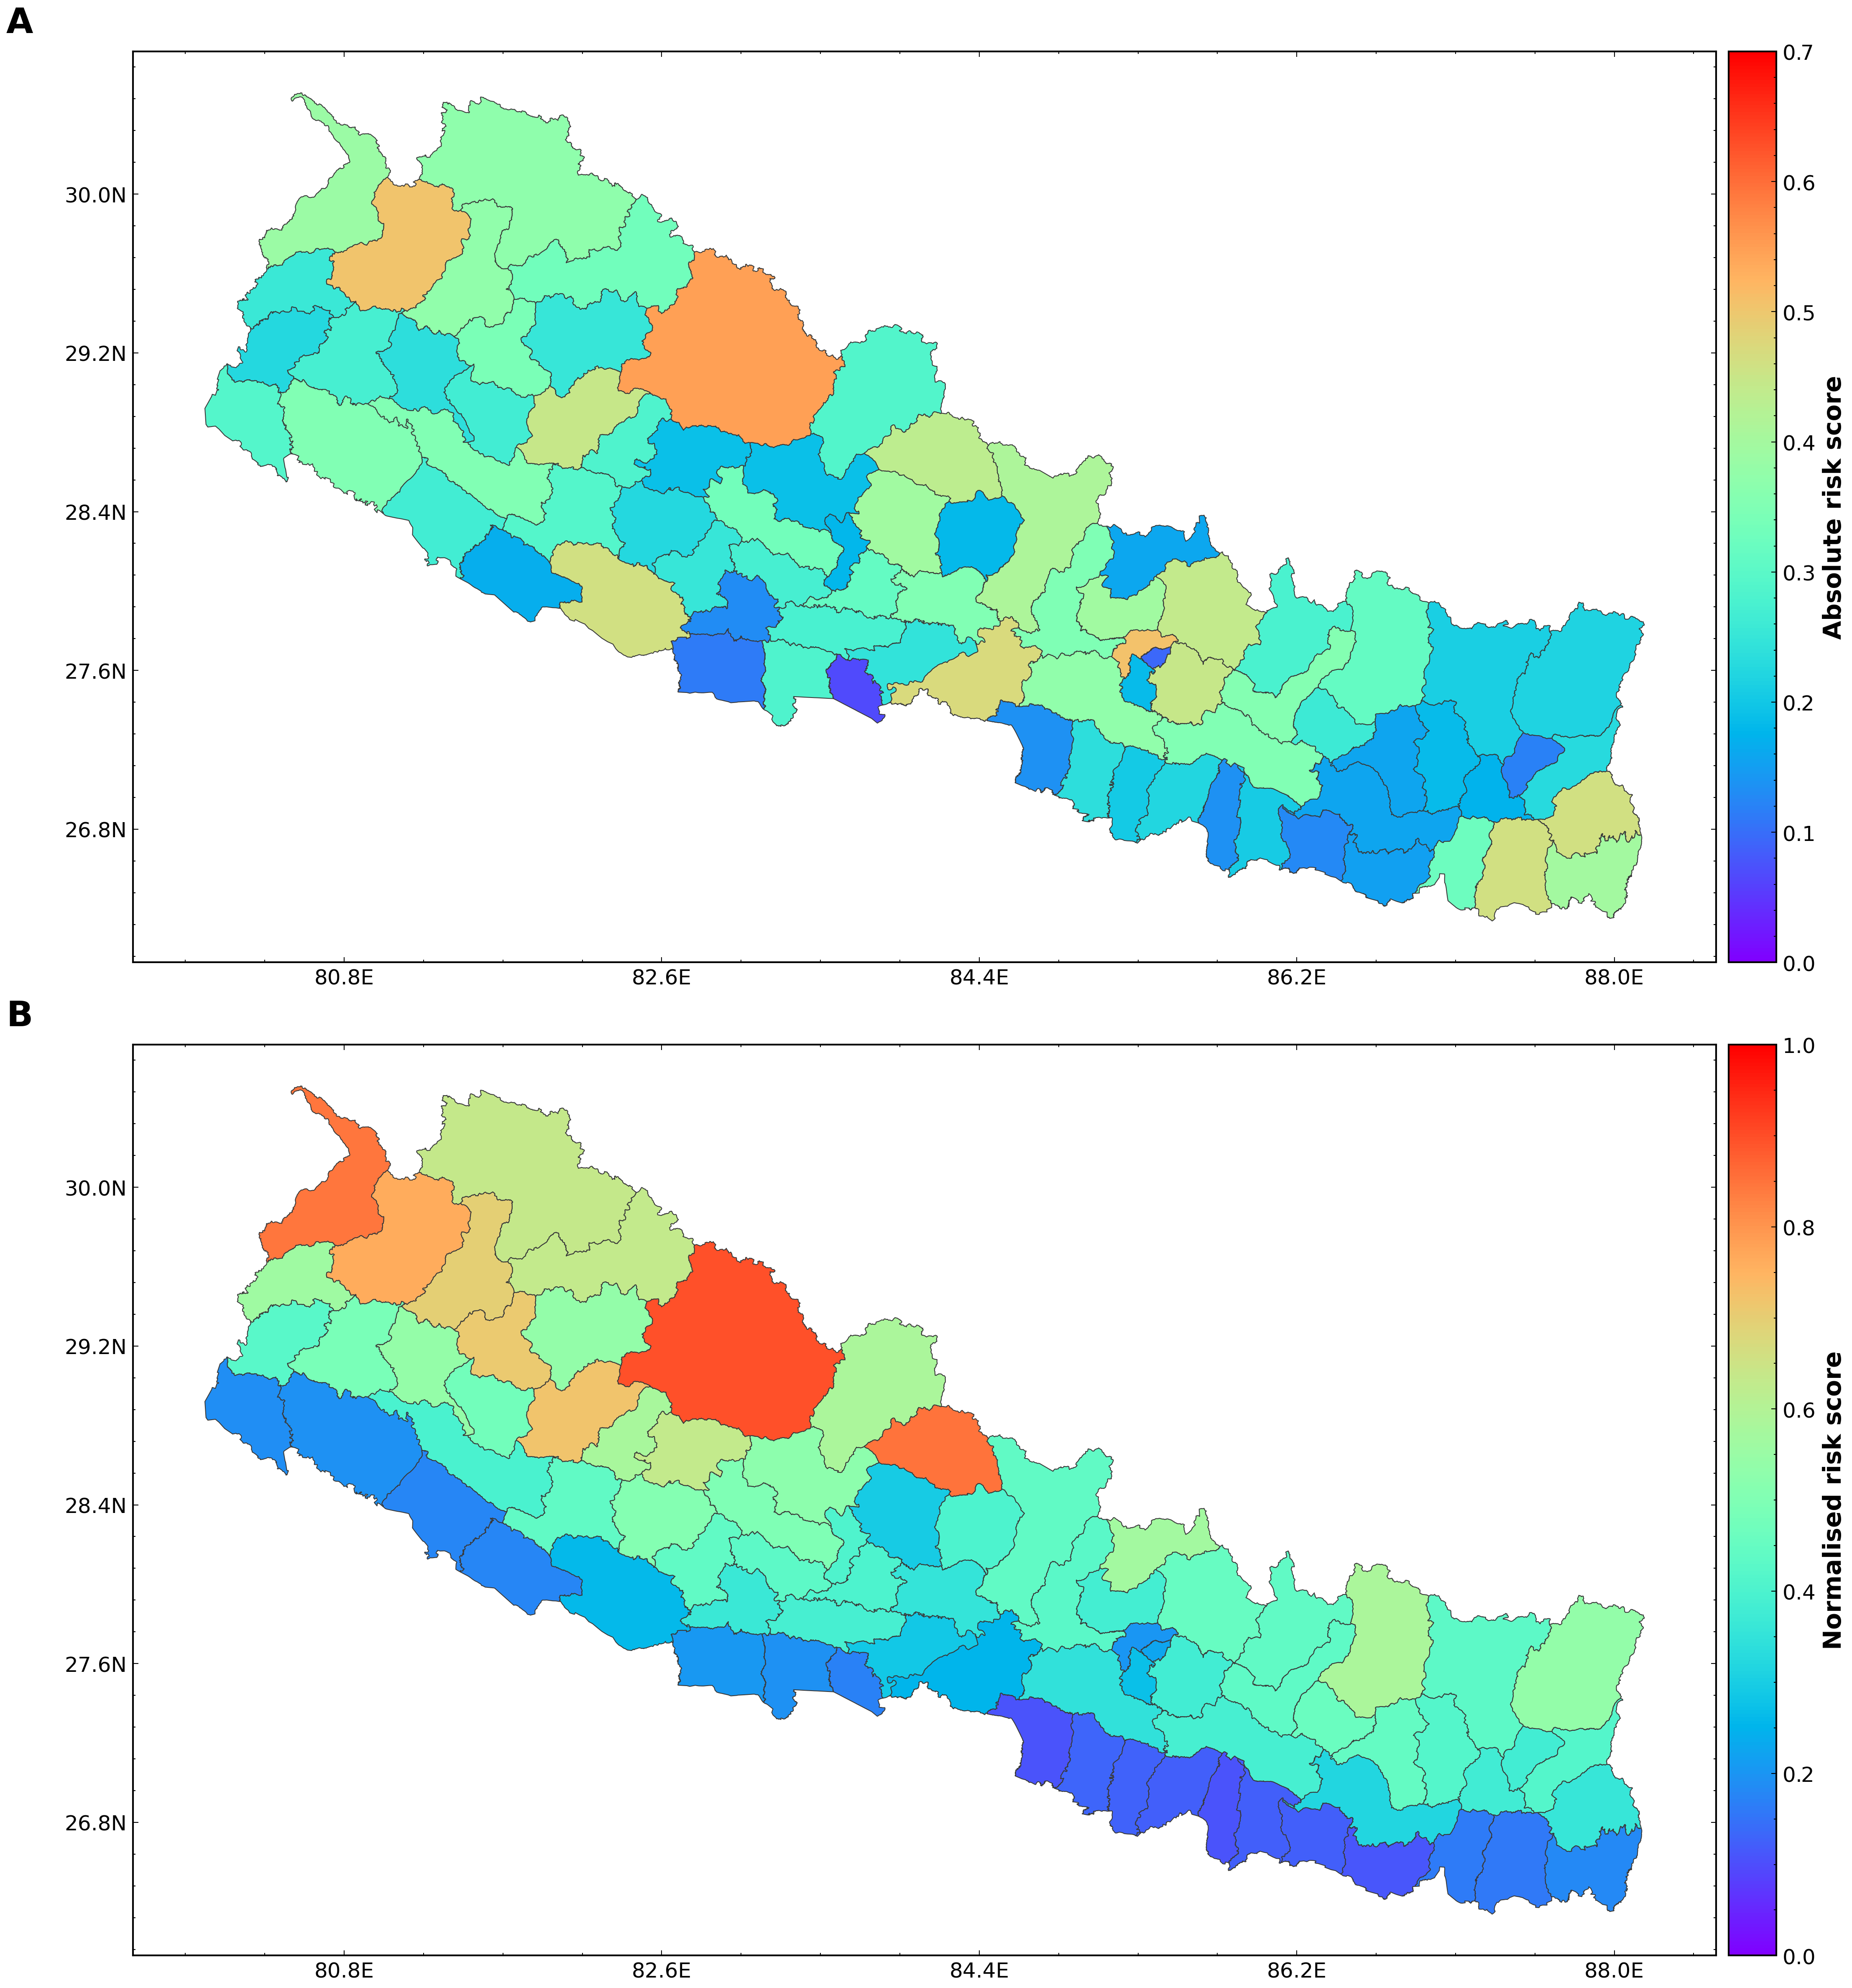
\includegraphics[width=1\linewidth]{./FIGURES/revised_v2/Fig8_risk_scores.png}
    \caption{Maps of multi-hazard risk scores. A, absolute risk score identifying hotspots of large-scale earthquake impacts. Note that these are variably distributed across the country and across physiographic divisions, reflecting the aggregate influence of remoteness, absolute impact numbers, or both. B, normalised risk score identifying districts where the community is most severely threatened regardless of size. Note that high scores are found predominantly in the hill and especially mountain districts, where remoteness is high and landslide impacts are proportionately more important.}
    \label{fig:risk_score}
\end{figure}

Figure \ref{fig:risk_score} illustrates how different risk metrics reveal distinct spatial patterns of earthquake risk across Nepal. The absolute risk score (Figure 8A) combines remoteness with total worst-case damage (buildings and roads). This metric identifies districts facing the largest aggregate disaster burden, with elevated scores scattered around Nepal, in districts such as Dolpa, Kathmandu, Bajhang, Chitawan, Dang and Morang. These areas score highly due to either substantial absolute infrastructure exposure, high remoteness, or both factors combined. In contrast, the normalised risk score (Figure 8B) accounts for proportional damage relative to each district's infrastructure and population size. This normalisation fundamentally shifts the risk geography, revealing acute risks in hill and mountain districts, especially in the north and northwest of the country, where communities face disproportionately high percentages of infrastructure loss in combination with high remoteness. 

\section{Discussion}

Our hypergraph model extends the earthquake scenario ensemble approach developed by Robinson et al. (2018) to include both primary hazards from earthquake shaking as well as secondary hazards from coseismic landslides. In a tectonic setting like Nepal, characterised by highly variable topography and a well-established chain of earthquake-related hazards \citep{Kincey2021}, this allows us to develop a fuller picture of the potential impacts in those future scenario earthquakes. We consider some of the key differences between the scenario ensemble results of Robinson et al. (2018) and our findings and their implications for humanitarian contingency planning, as well as the limitations of our approach.

\subsection{Differences between shaking-only and multi-hazard scenario outcomes}

Robinson et al. (2018) derived a normalised risk index based on worst-case earthquake-shaking impacts across their ensemble, combined with a measure of remoteness and with the Human Development Index (HDI) as a measure of social vulnerability, and used that to rank Nepal's 75 pre-2015 districts by risk (Figure~\ref{fig:robinson_comparison}C). It is useful to compare that shaking-only risk estimate with our normalised risk score shown in Figure~\ref{fig:risk_score}B, to assess whether the districts prioritised in contingency planning would change when considering the broader earthquake impacts that we model here. Direct comparison of the district-level rankings between the two risk models yields a Spearman rank correlation coefficient of 0.80 (Figure~\ref{fig:robinson_comparison}B), so the relative risk profile of Nepal's districts is broadly preserved at the national scale. This result is expected, because the two analyses share the same 30-member earthquake ensemble and shaking damage dominates total impact counts in the majority of districts. However, the overall correlation conceals meaningful divergence in specific districts (Figure~\ref{fig:robinson_comparison}A, C), particularly mountain districts along Nepal's northern border such as Manang, Rasuwa and Mustang, which rank 39--59 places higher in our score than in that of Robinson et al. (2018). Because the two scores also differ in how shaking damage is estimated, including the underlying building exposure data, in the basis for the remoteness scoring, and in the use of the HDI by Robinson et al. (2018), the differences in modelled output cannot be attributed to landsliding alone. Indeed, a shaking-only version of our normalised score (Equation~\ref{eq:normalized-risk-score} without the landslide term) has the same correlation with the score of Robinson et al. (2018) ($\rho = 0.80$), indicating that most of the divergence reflects these other differences between the two scores. To isolate the contribution of landslides, we therefore compare rankings with and without landslide impacts within our own results. In terms of worst-case impacts alone (Figure~\ref{fig:district_ratio}A), including landslide impacts moves several hill and mountain districts up the ranking by up to 8 places (Kalikot and Bajura; Section~\ref{sec:results_impacts}), so a shaking-only assessment would give these districts a lower priority for contingency planning than their total impacts warrant. The effect is stronger for our normalised score, which accounts for proportional damage: including the landslide term moves several hill and mountain districts substantially up the ranking, most notably Rasuwa (22 places), Baglung and Myagdi (12 places each), and Gulmi (8 places), while districts with little landslide damage relative to shaking move down (Figure~\ref{fig:robinson_comparison}C; Table~\ref{tab:S2}). These are the districts in which the multi-hazard approach adds most to a shaking-only assessment, consistent with the documented tendency of shaking-only frameworks to underestimate risk in areas of high topographic relief where secondary hazards are prevalent \citep{Budimir2014}. This reinforces the need for multi-hazard approaches that account for the full chain of earthquake-related impacts in continental earthquake settings.

\begin{figure}[H]
    \centering
    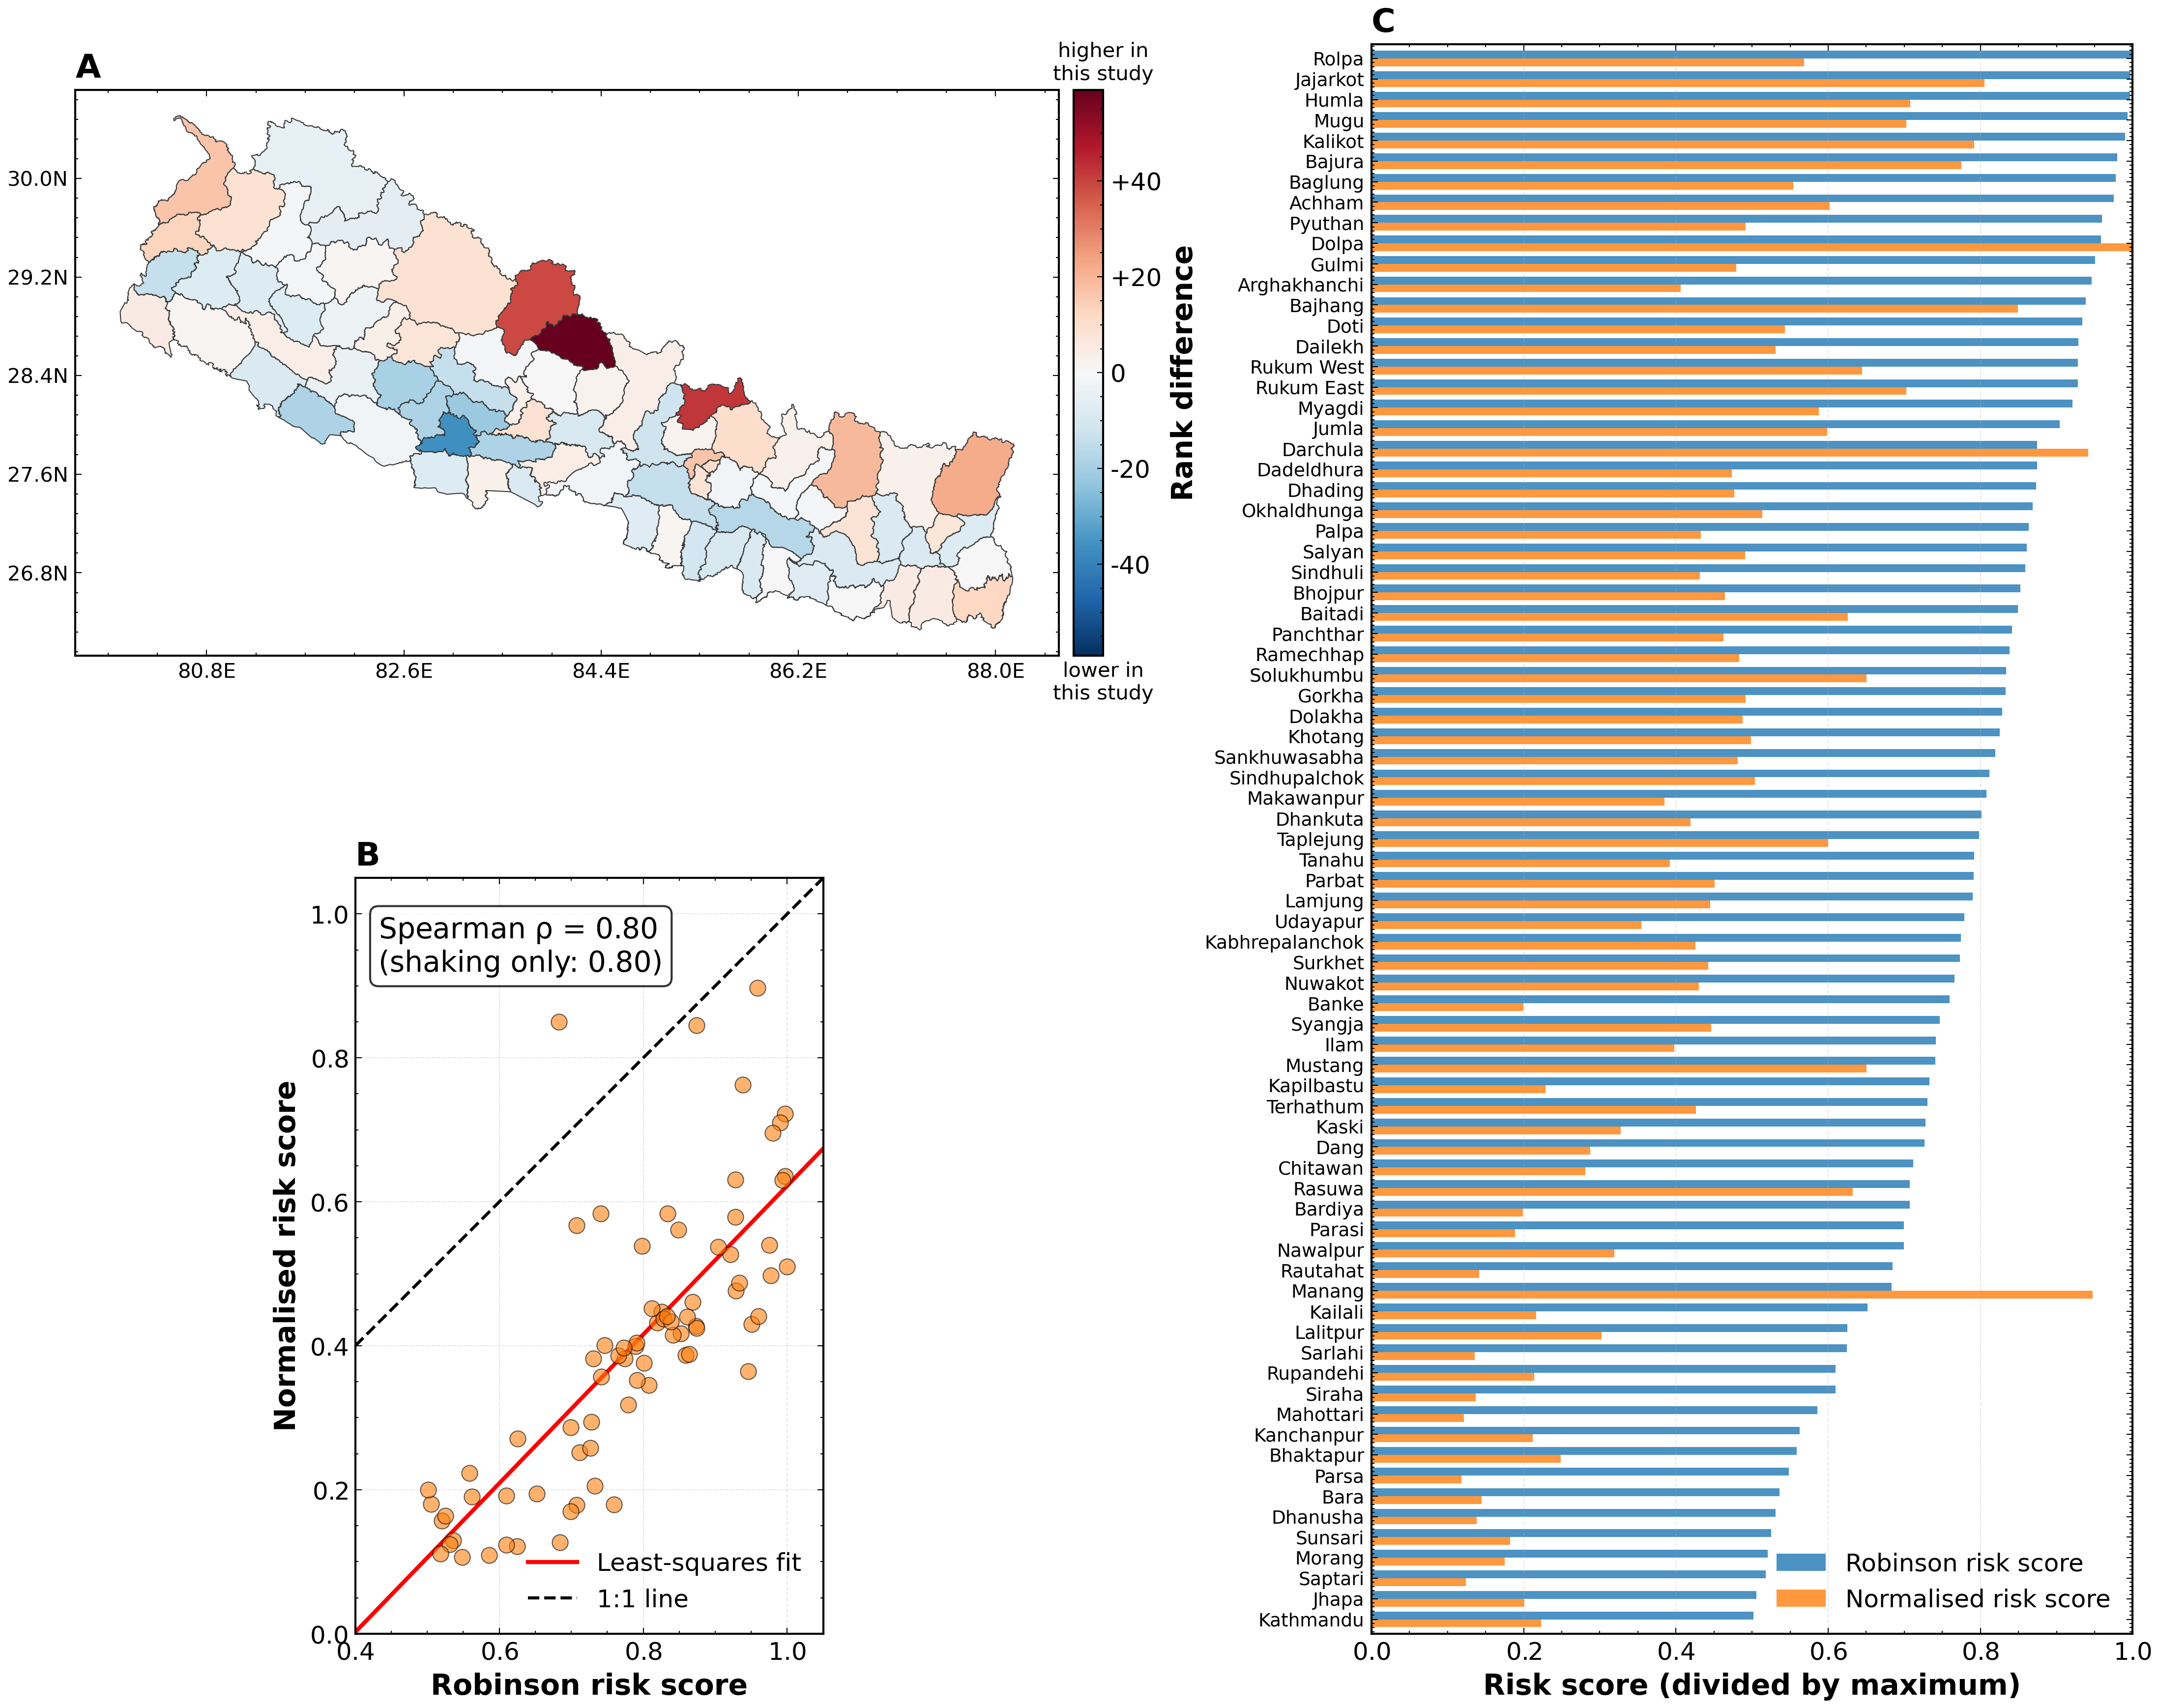
\includegraphics[width=1\linewidth]{./FIGURES/revised_v2/Fig9_robinson_comparison.png}
    \caption{District-wise comparison between normalised risk score derived here and the relative risk score proposed by Robinson et al. (2018), referred to here as 'Robinson risk score'. A, map of the difference between the rank of each district in the Robinson risk score and its rank in our normalised risk score (rank 1 = highest risk among the 77 districts). Positive values (red) indicate districts that rank higher, that is, at greater relative risk, in our score. The Robinson risk score is based on worst-case earthquake shaking impacts combined with remoteness and the Human Development Index (HDI), and is adapted here to the current district outlines. Note that the largest upward shifts are found in mountain districts along the northern border, such as Manang, Mustang and Rasuwa. B, scatter plot of district-level risk scores from the two models. The red line shows a linear least-squares regression, while the black dashed line shows a 1:1 relationship for reference. We find a Spearman rank correlation coefficient of 0.80 between the two datasets (n = 77 districts); a shaking-only version of our normalised score gives the same value (0.80). Scores of Robinson et al. (2018) for Nawalparasi and Rukum are assigned to both of their successor districts (Nawalpur and Parasi; Rukum East and Rukum West). C, district-wise plot of risk scores in the two models, each divided by its maximum value. Bars are ordered by the Robinson risk score. While the two datasets have similar overall trends in their relative values, there are some notable outliers, especially for mountain districts in northern and northwestern Nepal.}
    \label{fig:robinson_comparison}
\end{figure}

The spatial variability in the ratio of landslide to shaking damage (Figure~\ref{fig:district_ratio}) further highlights the role of landslide susceptibility, and thus of local topography, in shaping district-level impact patterns. Districts in the low-relief Terai show consistently low landslide contributions, while northern mountain districts such as Darchula, Manang, and Dolpa show the highest ratios. This heterogeneity implies that risk thresholds derived from aggregated national or regional statistics will systematically misrepresent the relative severity of risk in topographically complex settings, and that multi-hazard assessments that resolve differences in landslide susceptibility and exposure at district or finer scales, rather than relying on national or regional averages, are necessary to support effective contingency planning across diverse physiographic regions like Nepal.

\subsection{Road network impacts and compounding effects of remoteness}

The quantification of landslide damage to the road network represents one of the most operationally significant contributions of this study relative to previous scenario ensemble approaches for Nepal. Road infrastructure is the primary means of access for emergency responders, medical and relief supplies, and humanitarian personnel in Nepal's hill and mountain districts, and its disruption following a large earthquake can substantially delay response times and compound the human consequences of the event \citep{Koks2019, NationalPlanningCommission2015}. Our results show that the proportion of the road network damaged by landslides is substantially higher in districts classified as highly remote (median $\approx 20\%$) than in those with low remoteness (median $\approx 9\%$), and this disparity is compounded by the fact that remote districts already face longer pre-event travel times to health facilities and district headquarters (Figure~\ref{fig:remoteness}). This result is perhaps to be expected, because the steep terrain that makes these districts remote also makes them susceptible to landsliding. Its importance lies in the fact that remote districts also have sparse road networks with few alternative routes, so damage to a given proportion of road segments is more likely to cut off access than in districts with denser, more redundant networks. The two effects are likely to reinforce each other: the steep, high-relief terrain that elevates landslide susceptibility is also what makes post-event access most critical and most difficult to restore. Districts such as Dolpa, Bajhang, and Darchula illustrate this compound risk most acutely, combining high remoteness with worst-case landslide damage to 17--29\% of road segments. Here, we treat all road segments equally, irrespective of road class or of the density of the road network in each district. Weighting road segments by their class (e.g., strategic highways versus local roads) or by their role in network connectivity would be a straightforward extension of the model, and would help to distinguish road damage that has different consequences for emergency response.

These findings have direct implications for pre-event contingency planning. The identification of districts where road damage is both severe and consistent across multiple scenarios provides a basis for prioritising alternative access options, including pre-positioning of emergency supplies and response capacity \citep{Sijapati2024}, the development of secondary route alternatives, and planning for aerial transport logistics in the most inaccessible areas. In districts where extensive landslide damage to roads is likely in a large earthquake, post-event road access cannot be assumed, and pre-event preparation is correspondingly critical \citep{IASC2007}.

\subsection{Scale dependence of hazards}

The importance of secondary hazards such as landsliding, relative to primary earthquake shaking, varies substantially with spatial scale and underlying exposure patterns. In densely populated districts with large numbers of buildings and low topographic relief, landslide impacts represent a small addition to shaking damage, sitting at the lower end of the 1--84\% range observed across all districts (Figure~\ref{fig:district_ratio}). However, in mountainous districts with steep terrain and relatively few buildings and road segments, landslide impacts on buildings and roads can reach 84\% of the number of buildings damaged by shaking (Figure~\ref{fig:district_ratio}). While landslides account for a small fraction of national-level damage -- with national totals for each type of landslide impact one to two orders of magnitude below shaking impacts (Figure~\ref{fig:exceedance}) -- they have the potential to nearly double the impacts in specific localities, transforming what would otherwise appear as a moderate shaking scenario into a much more damaging multi-hazard event. Planning frameworks that rely solely on national or regional statistics may therefore systematically underestimate risk in localities where cascading hazards dominate.

\subsection{Urban--rural risk contrast and geographic disparities}

The results are consistent with a spatially structured urban--rural risk divide, with direct implications for disaster risk governance in Nepal. Urban and peri-urban districts in the Terai and major river valleys face the greatest absolute burden from earthquake shaking, a consequence of their high population density, building stock and exposure to secondary hazards. However, the most severe proportional losses -- and likely the greatest challenges for post-event response -- are concentrated in remote rural districts of the hill and mountain areas. These districts face disproportionately high percentages of road damage in combination with high remoteness from health facilities and government support (Figures~\ref{fig:worst_case_maps} and \ref{fig:remoteness}). Although we do not model recovery capacity directly, longstanding disparities in infrastructure investment and institutional capacity across Nepal's physiographic regions \citep{NationalPlanningCommission2014} suggest that the communities whose physical connectivity is most vulnerable to earthquake-triggered landslides may also be among those least equipped to absorb and recover from disaster impacts. The persistence of such geographic inequalities in disaster risk and response capacity has been widely documented across multi-hazard settings \citep{Wisner2004}.

Our results also show clear spatial differences in how much earthquake-related impacts vary between scenarios, as measured by the standard deviation across the 30 scenario earthquakes (Figure~\ref{fig:standard_deviation}A, C, E). Low standard deviation in building damage from earthquake shaking (Figure~\ref{fig:standard_deviation}A) is to be expected in western Nepal, simply because of the smaller number of buildings in those districts. For landslide impacts, however, the largest variability is found in hill and mountain districts of central and western Nepal, such as Sindhupalchok, Baglung, Bajhang, Rolpa and Jajarkot (Figure~\ref{fig:standard_deviation}C, E), pointing to the potential for localised but highly disruptive impacts in specific individual modelled earthquake scenarios. In these areas, contingency planning for median or `typical' earthquake impacts may thus obscure a real and important distinction between the majority of events in the ensemble, which have limited impact, and a few earthquakes that can have locally severe effects. The 2023 Mw 5.7 Jajarkot earthquake provides a potential illustration; despite its moderate size, it killed 154 people and damaged approximately 62,000 households, affecting about 250,000 people \citep{UNRCO2024}. In districts such as these, where landslide impacts vary strongly between scenarios, it is especially important to plan for the worst-case future event. Relative to their typical level, landslide impacts are instead most variable in Terai districts such as Banke, Bardiya, Siraha and Saptari (coefficient of variation up to 2.85; Figure~\ref{fig:standard_deviation}D, F), where impacts are small and occur in only a few scenarios. The coefficient of variation therefore highlights where impacts are rare rather than where they are large, and the absolute spread shown in Figure~\ref{fig:standard_deviation}A, C, E is the more relevant measure for planning response capacity.

\subsection{Limitations}
\label{sec:limitations}

Several limitations are inherent to the ensemble approach. While the analysis captures large-scale impacts from high-magnitude earthquakes ($M_w > 7$), it does not include the effects of locally destructive moderate-magnitude events such as the 2023 Jajarkot earthquake. As mentioned above, these events can cause severe localised impacts and warrant dedicated modelling efforts. While they could be included in an enhanced scenario ensemble, the number of potential earthquake sources and locations increases dramatically as the minimum scenario magnitude decreases (Robinson et al., 2018). In addition, we focus here on physical infrastructure damage and do not explicitly model fatalities, as infrastructure impact alone is not sufficient for risk-to-life estimates from landslides \citep{VanWykDeVries2024}. Future work integrating dynamic exposure and population mobility data is expected to improve casualty estimation for both shaking and landslide hazards.

A further limitation concerns the transferability of the susceptibility and fragility models across the ensemble. Both the landslide susceptibility model and the building fragility functions were calibrated using observations from the 2015 $M_w$ 7.8 Gorkha earthquake, which involved thrust rupture on the Main Himalayan Thrust beneath central Nepal. Several of the 30 scenario earthquakes considered here involve different fault systems and fault slip orientations -- including the Karakoram Fault and the Thakkhola Graben -- for which no independent calibration data on earthquake-triggered landslides are currently available. The degree to which the susceptibility and fragility relationships derived from the Gorkha event can be generalised to these different tectonic and geomorphic settings is uncertain and represents an important topic for future investigation.

It is also important to note that the hypergraph model as described here accounts only for earthquake shaking and coseismic landslides. Thus, there is no consideration of either enhanced post-seismic landsliding, or the reactivation and evolution of the spatial footprint of pre-seismic and coseismic landslides by post-earthquake rainfall \citep{Kincey2021,Kincey2023,Shrestha2026}. As a result, the modelled impacts shown here should be taken as an estimate of impacts that could be expected to occur on the day of a future earthquake, and are highly likely to be minima compared to the full time-integrated inventory of both coseismic and post-seismic impacts. Recent work by \citet{Harvey2026} on an extended 30-year multi-temporal inventory of landsliding in Nepal has shown that, at the scale of the entire country, the Gorkha earthquake produced only a small increase in the total coverage of landslides across Nepal. They also showed that, at any given time, c. 80 percent of landslide area in Nepal was visible in the preceding year, implying that most of that landslide area represents reactivated events rather than entirely new failures. Thus, our use of susceptibility - which by definition indicates the most likely areas of new landslide occurrence - underestimates the potential landslide footprint in a future earthquake. Future iterations of the hypergraph model could incorporate runout from existing landslides \citep[e.g.,][]{Kincey2023} alongside coseismic landsliding, in order to close this gap.

Finally, we report expected district-level impacts, which do not depend on whether damage to individual buildings and road segments is independent. In practice, co-location of multiple assets within large landslide source or runout areas introduces positive spatial correlation in outcomes, which widens the range of impacts that could occur within a single scenario, particularly in districts with large, contiguous slope units. Because we do not report this within-scenario spread, future work that characterises the full distribution of outcomes, including spatially correlated failures, would help to quantify this additional source of uncertainty.


\section{Conclusions}

This study extends scenario ensemble-based earthquake risk assessments by incorporating coseismic landslide hazards into the scenario framework developed by \cite{Robinson2018}. We have leveraged the hypergraph method for cascading scenario generation developed by \cite{Dunant2025} and applied it to a suite of 30 potential future earthquakes in Nepal. The resulting multi-hazard ensemble reveals that landslides substantially increase impacts in steep and remote regions of Nepal. Although landslides account for a small proportion of total building damage compared to shaking, their contribution to overall risk is substantial. In hill and mountain districts, worst-case landslide impacts on buildings and road segments can exceed 50\% of the worst-case number of buildings damaged by shaking, indicating that landslide damage can be a critical additional component of earthquake damage under specific scenarios. This underscores the spatial heterogeneity in hazard impacts across the country.

The analysis also illustrates how landslides can significantly affect transport infrastructure, particularly in remote areas, which could reduce access to both government services and health care facilities in addition to complicating emergency response. The strong correlation between remoteness and anticipated road damage highlights the importance of pre-event planning and infrastructure resilience, as emphasised in national frameworks such as the Earthquake Response Preparedness Plan (ERPP). The current ensemble does not account for moderate-magnitude (Mw 5-6) but locally destructive events, such as the 2023 Jajarkot earthquake. This points to the need for complementary localised modelling approaches to capture risk in under-represented areas.

Finally, the findings are consistent with a persistent urban--rural risk divide, shaped by geographic and infrastructural disparities. Addressing this divide remains a key priority for disaster risk reduction. Future improvements in fatality modelling and the integration of high-resolution mobility and exposure data will be essential for producing more accurate and actionable multi-hazard risk assessments.

\section*{Acknowledgments}
This research was supported by a grant from the UKRI Global Challenges Research Fund via the Multi-Hazards and Systemic Risk programme (grant NE/T01038X/1: www.sajag-nepal.org). The AW3D DEM is licensed via Durham University (UK), with funding from the DFID-UKRI SHEAR programme (project number: 201844-112) (AW3D 5 m DEM \textcopyright JAXA, RESTEC and NTTDATA). We are grateful to successive UN Resident Coordinators in Nepal for their continuing support and engagement, and to representatives of the humanitarian clusters that comprise the Humanitarian Country Team in Nepal for their guidance that helped to shape this research. R.M.R. and S.H. affirm that this work was undertaken in a personal academic capacity and does not represent the views of the United Nations. The shaded-relief basemap in Figure~\ref{fig:study} is from Esri World Shaded Relief (tiles \textcopyright{} Esri).

\section*{Author Contributions}
ALD, TRR, NJR, and others secured the funding for the research reported here. The study was conceived by AD, TRR, ALD, and NJR. AD developed the numerical model with input from TRR, ALD, NJR, RMR, SH, and MK. AD ran the numerical experiments with assistance from TRR and RMR. AD, ALD, and TRR wrote the original draft of the manuscript. All authors contributed to analysis of the results and review and editing of the manuscript.

% -------------------- REFERENCES --------------------
% The following command will include references from references.bib
\bibliography{references}

% -------------------- SUPPLEMENT --------------------
\clearpage
\appendix
\renewcommand{\thefigure}{S\arabic{figure}}
\setcounter{figure}{0}

\section*{Supplemental Information}

\begin{figure}[H]
    \centering
    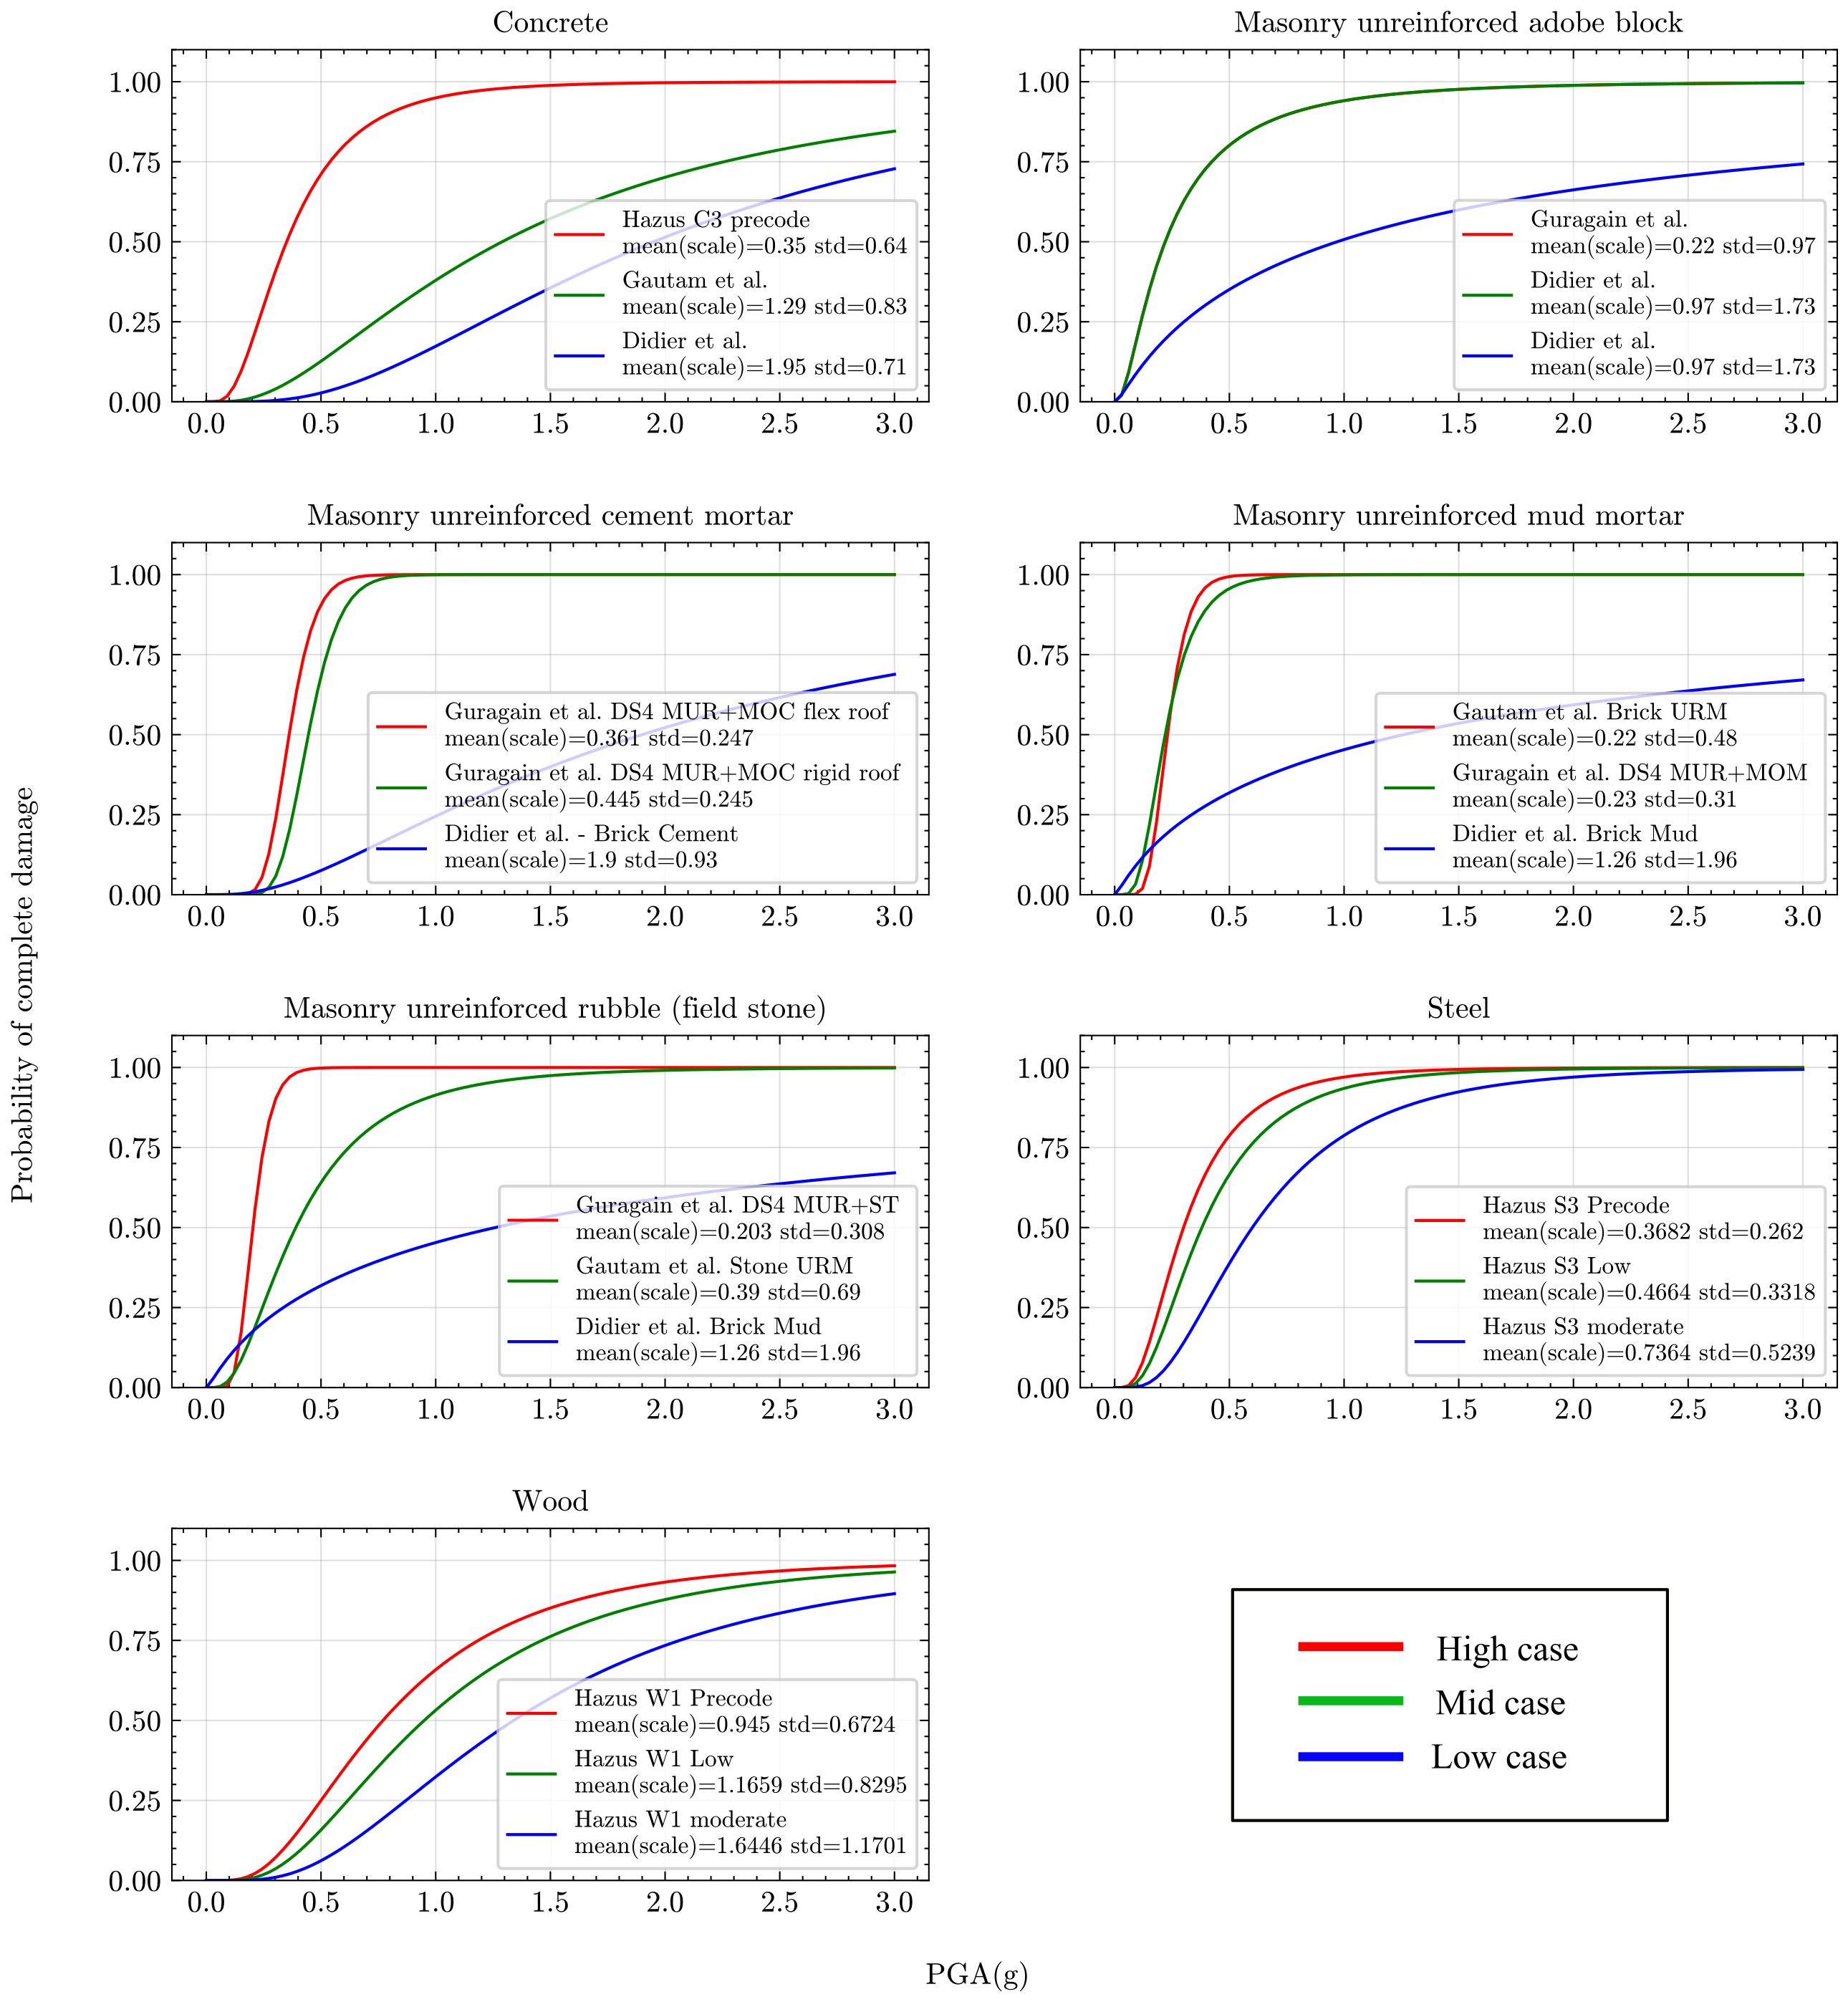
\includegraphics[width=1\linewidth]{./FIGURES/FigS1_fragility_functions.png}
    \caption{Fragility functions used in the hypergraph network modelling, modified from Dunant et al. (2025). Each panel shows the functions for a different building type in the METEOR dataset (https://maps.meteor-project.org/map/building-exposure-map-of-nepal), relating peak ground acceleration (PGA, in g) to the probability of a complete damage state. Note that each fragility function is defined by two parameters: a scale parameter that sets the PGA value for 50\% probability of complete damage, and a standard deviation (std) that defines the spread of the curve. Parameter values and sources for the fragility curves are included in the plots \citep{FEMA2020Hazus, Didier2017, Gautam2018, Guragain2021}. For the experiments shown here, we adopt the mid case for each building type; see Dunant et al. (2025) for discussion}
    \label{fig:S1}
\end{figure}

\begin{figure}[H]
    \centering
    \includegraphics[width=0.75\linewidth, height=17cm]{./FIGURES/FigS2_pga_ensemble_maps.png}
    \caption{Maps of peak ground acceleration (PGA, in g) for each of the 30 scenario earthquakes in the ensemble. Earthquake name codes match those defined by Robinson et al. (2018).}
    \label{fig:S2}
\end{figure}

% Order swapped (comment C056): the silhouette figure is cited first in the text, so it now
% appears as Figure S3 and the median collapse maps as Figure S4. File names are unchanged.
\begin{figure}[H]
    \centering
    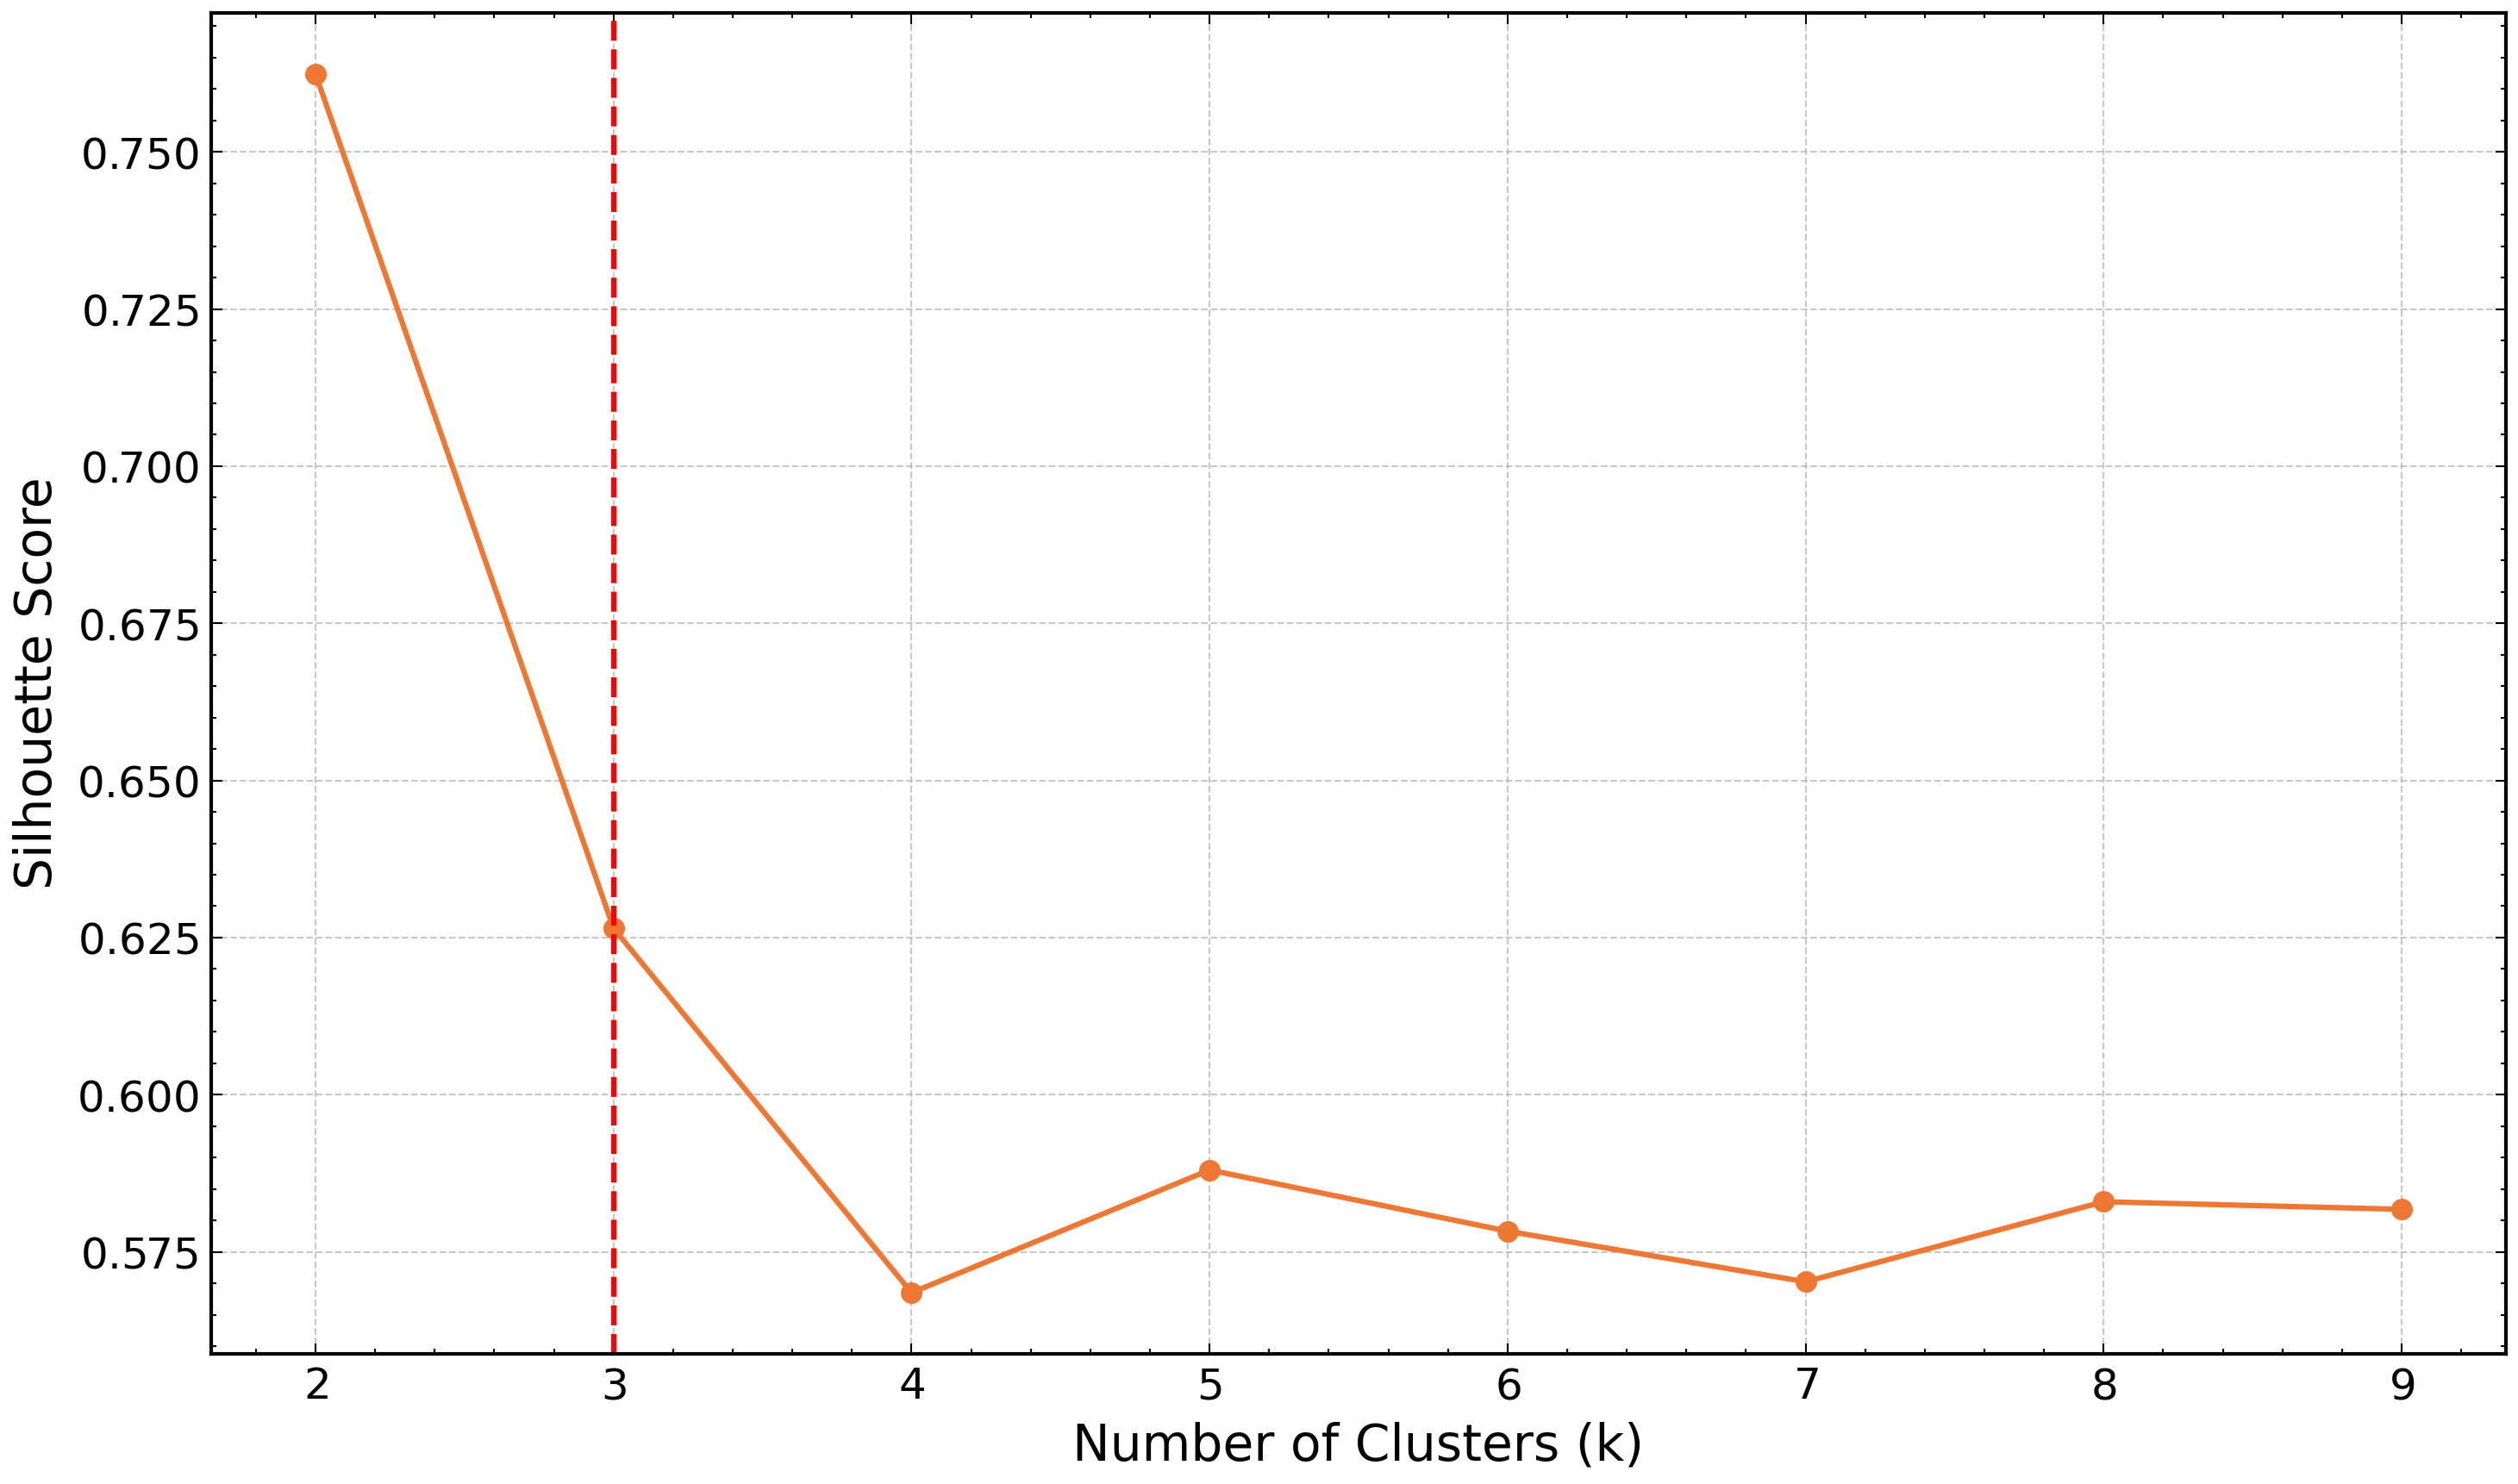
\includegraphics[width=1.0\linewidth]{./FIGURES/FigS4_remoteness_clusters.png}
    \caption{Silhouette scores for K-means clustering of the district remoteness index (access to district headquarters, dry season) with $k = 2$--9 clusters. The dashed line marks the three clusters retained for interpretability.}
    \label{fig:S4}
\end{figure}

\begin{figure}[H]
    \centering
    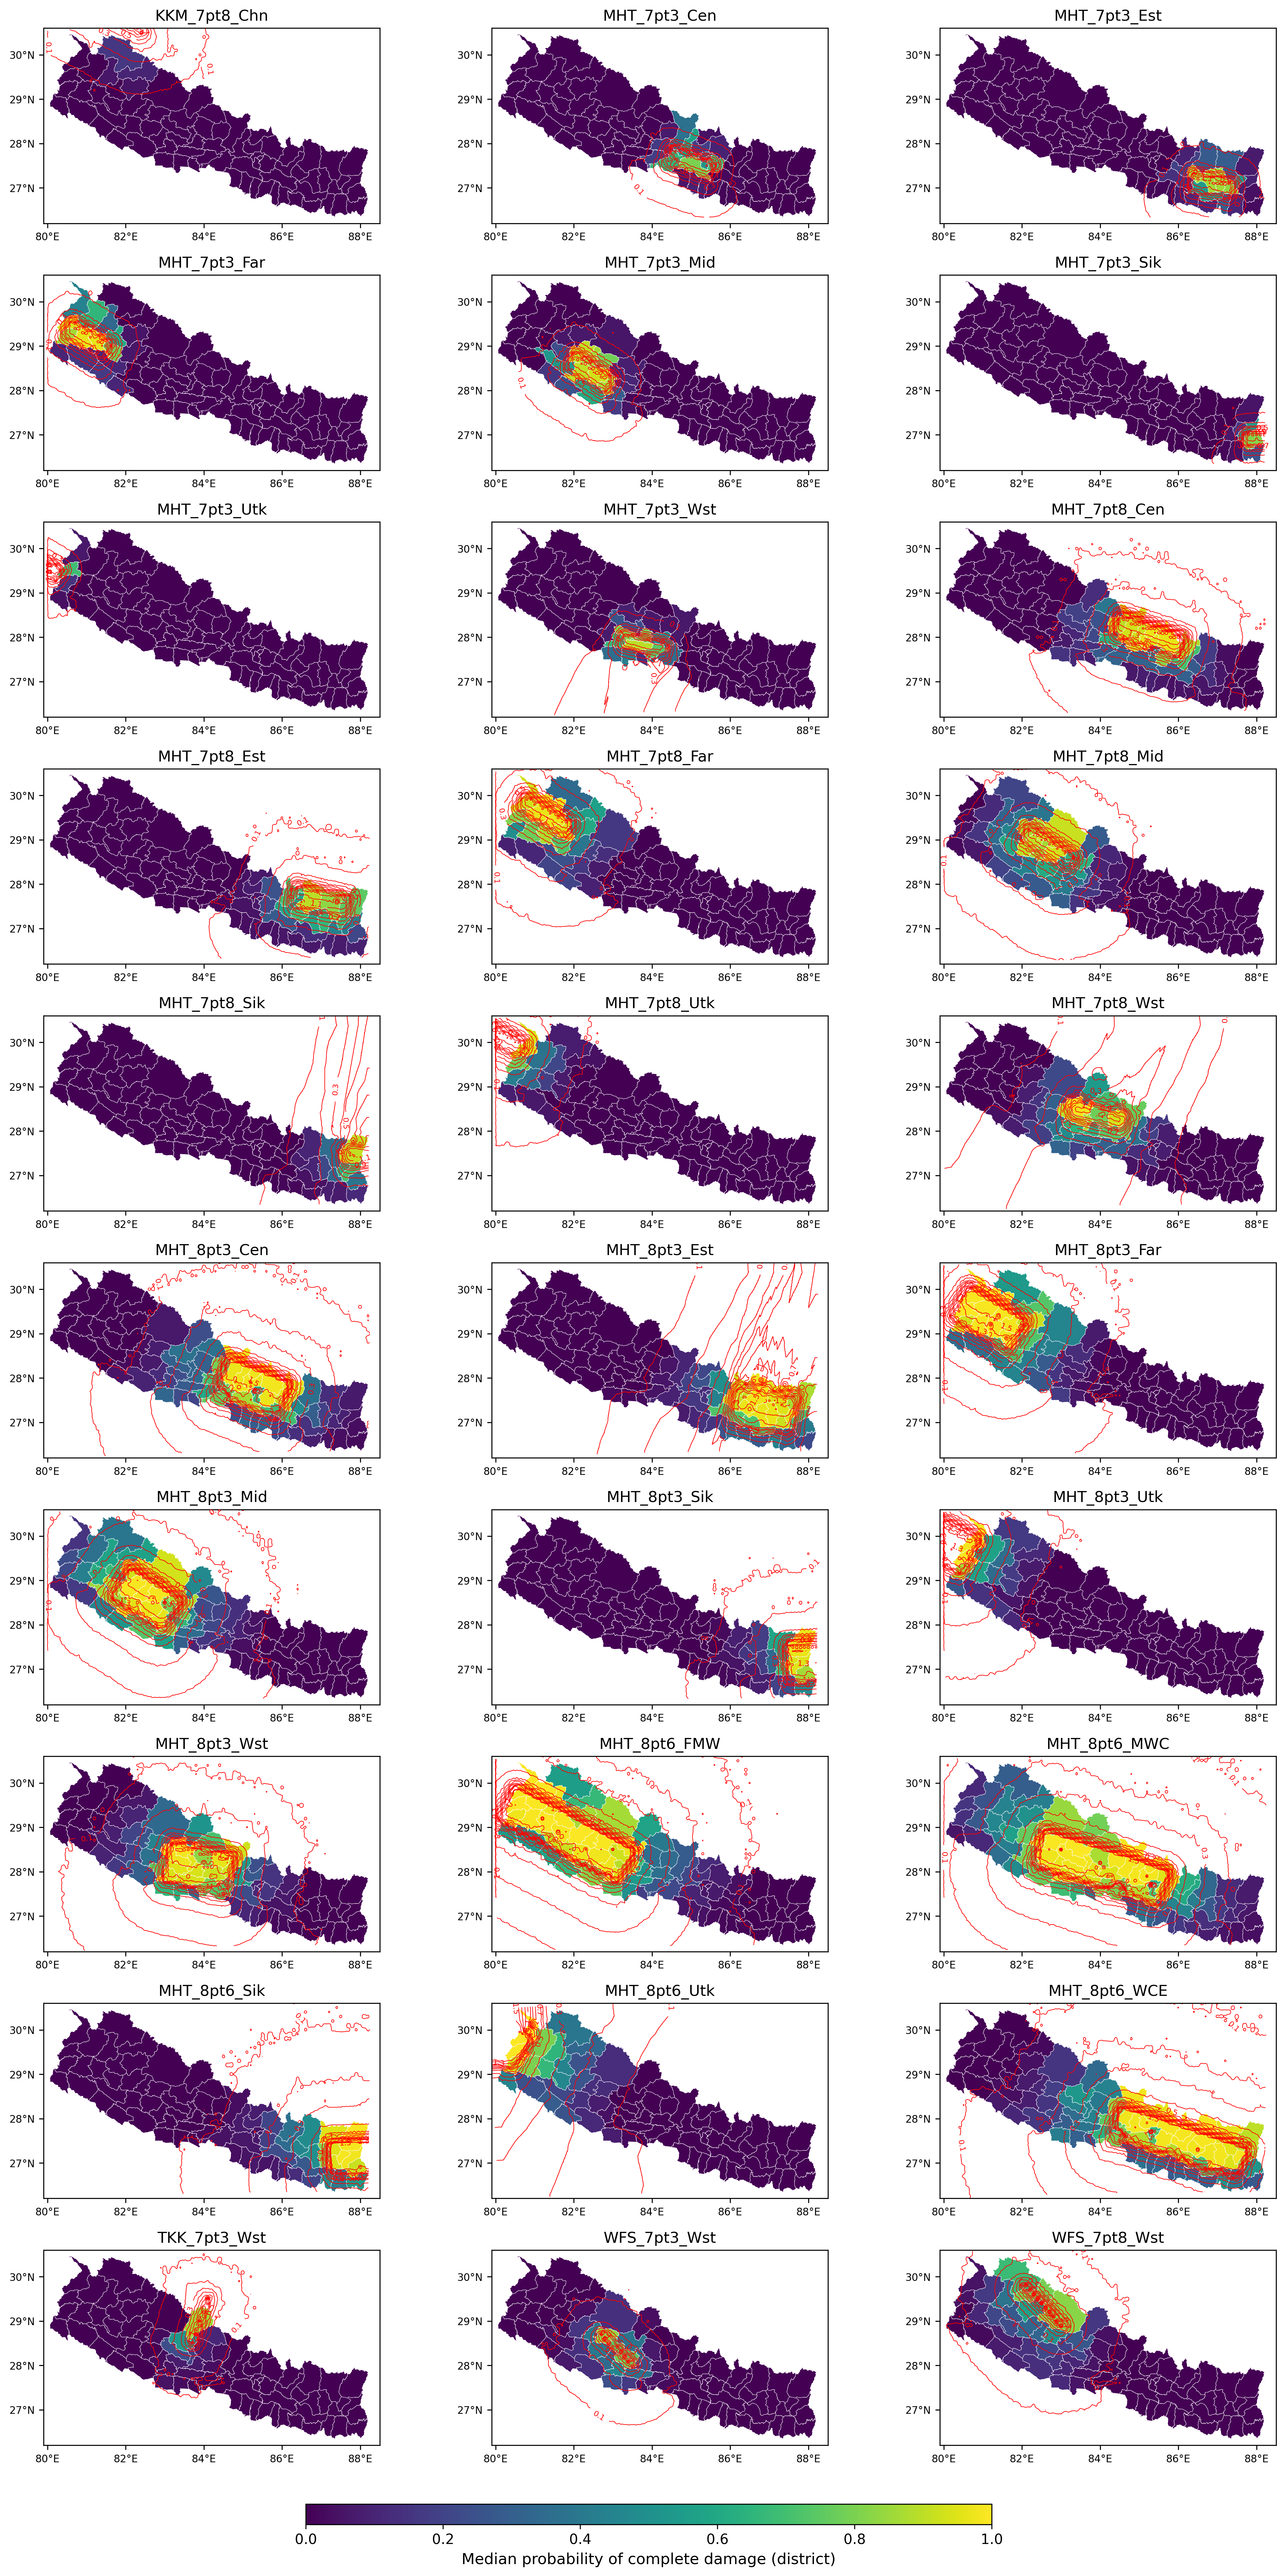
\includegraphics[width=0.75\linewidth, height=17cm]{./FIGURES/FigS3_median_collapse_probability.png}
    \caption{Maps of the median probability of complete damage in each district for each of the 30 scenario earthquakes in the ensemble. The probability of complete damage is modelled for each $90 \times 90$~m grid cell of the METEOR exposure dataset using the middle-case fragility functions (Figure~\ref{fig:S1}), and the median of these cell values is shown for each district \citep{Dunant2025}. Red contours show peak ground acceleration (PGA, in g).}
    \label{fig:S3}
\end{figure}

% New SI figure (comment C034): key map with the names of all 77 districts
\begin{figure}[H]
    \centering
    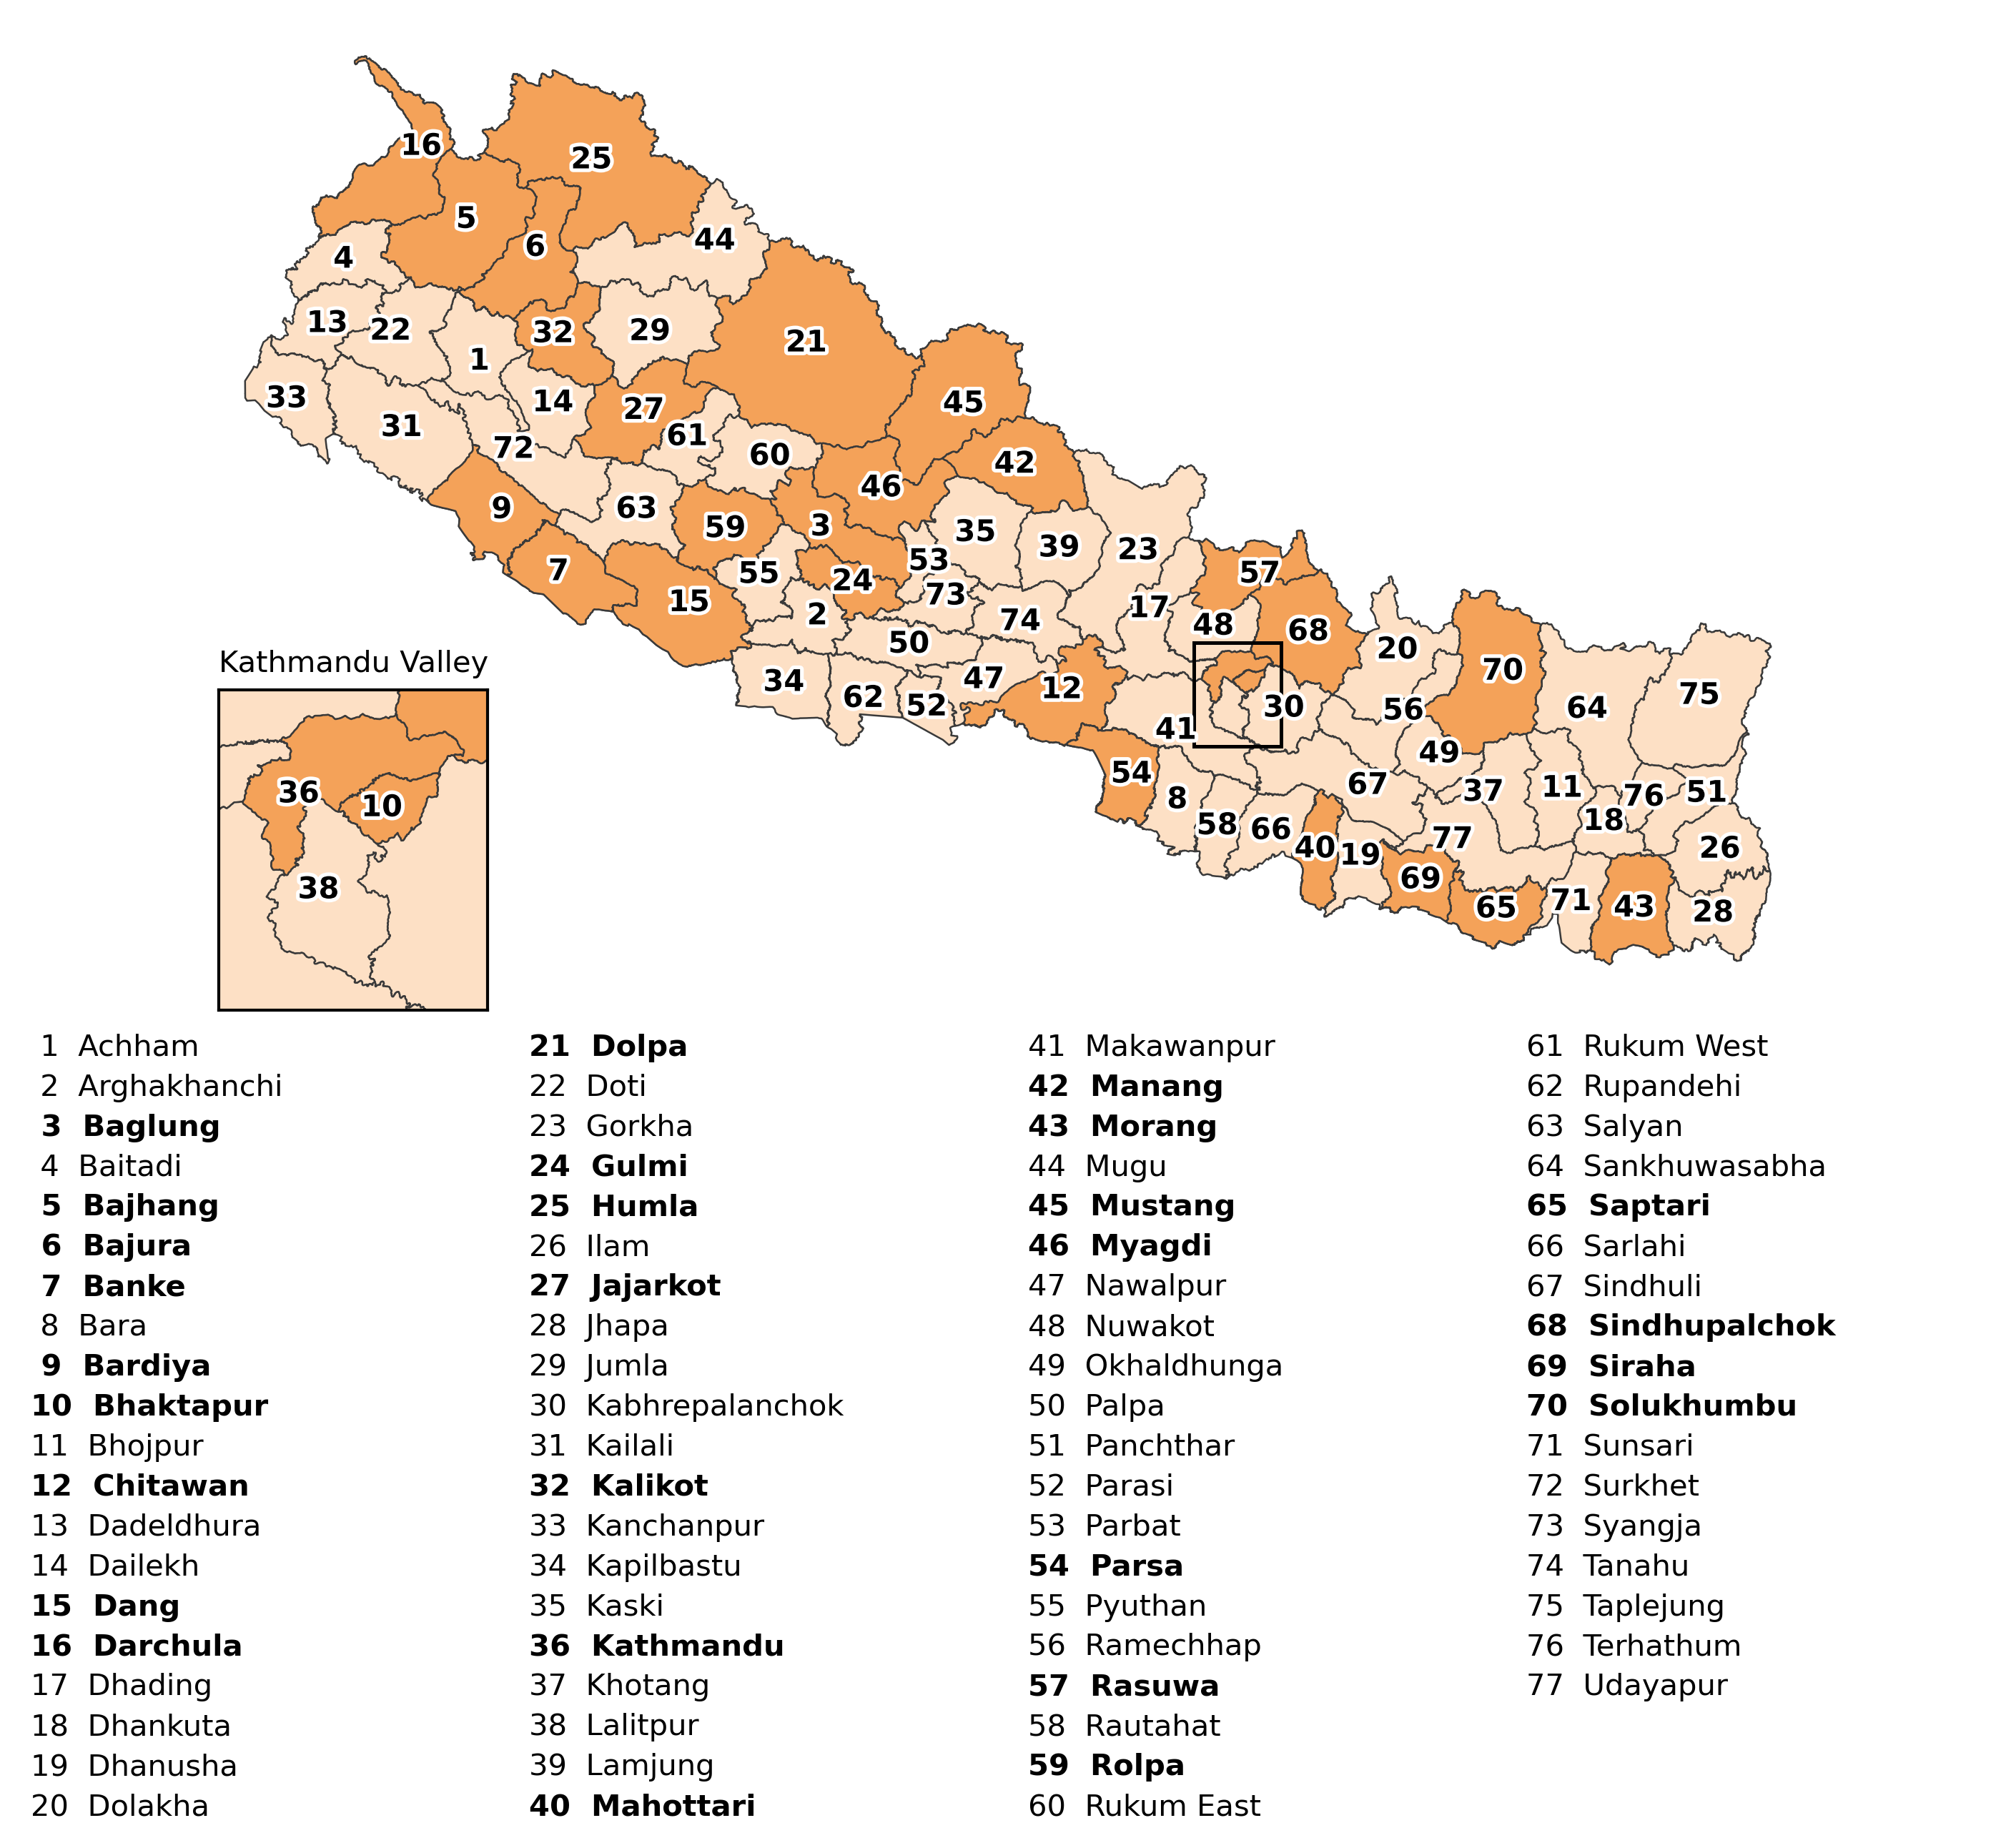
\includegraphics[width=1.0\linewidth]{./FIGURES/revised_v2/FigS5_district_names.png}
    \caption{Districts of Nepal, numbered alphabetically. Districts discussed in the main text (labelled in Figure~\ref{fig:study}) are shaded darker and shown in bold in the key. The inset shows the three districts of the Kathmandu Valley.}
    \label{fig:S5}
\end{figure}


\renewcommand{\thetable}{S\arabic{table}}
\setcounter{table}{0}

\begin{table}[H]
    \centering
    \caption{Sensitivity of the district rankings to the weights in the risk scores. Each alternative is compared with the score used in the main text (Equations~\ref{eq:absolute-risk-score} and \ref{eq:normalized-risk-score}): Spearman rank correlation across the 77 districts, largest change in the rank of any district, and number of districts shared by the two lists of the ten highest-ranked districts. For the absolute score, the road-segment weight sets how many buildings one damaged $100\,\text{m}$ road segment counts as (1 in the main text); R/S/L are the weights of remoteness, shaking and landslides in the normalised score (0.50/0.25/0.25 in the main text).}
    \label{tab:S1}
    \small
    \setlength{\tabcolsep}{5pt}
    \begin{tabular}{lccc}
        \toprule
                    & Spearman & Max.\ rank & Top-10  \\
        Alternative & $\rho$   & shift      & overlap \\
        \midrule
        \multicolumn{4}{l}{\textit{Absolute score}} \\
        \quad Buildings only (no roads) & 0.998 & 5  & 9  \\
        \quad Road segment = 0.5 bldg.  & 0.999 & 3  & 9  \\
        \quad Road segment = 2 bldgs.   & 0.997 & 5  & 10 \\
        \quad Remoteness weight 0.4     & 0.969 & 15 & 8  \\
        \quad Remoteness weight 0.6     & 0.966 & 16 & 6  \\
        \addlinespace
        \multicolumn{4}{l}{\textit{Normalised score (R/S/L)}} \\
        \quad 0.33/0.33/0.33 & 0.993 & 9 & 8  \\
        \quad 0.40/0.30/0.30 & 0.997 & 6 & 9  \\
        \quad 0.60/0.20/0.20 & 0.998 & 5 & 9  \\
        \quad 0.50/0.35/0.15 & 0.997 & 6 & 10 \\
        \quad 0.50/0.15/0.35 & 0.998 & 4 & 10 \\
        \bottomrule
    \end{tabular}
\end{table}

\begin{table}[H]
    \centering
    \caption{Districts whose rank in the normalised risk score changes by at least eight places when the landslide term is added to a shaking-only version of the score (rank 1 = highest risk among 77 districts). Positive changes indicate a higher ranking once landslides are included. District locations are shown in Figure~\ref{fig:S5}.}
    \label{tab:S2}
    \begin{tabular}{lccc}
        \toprule
        District & Rank, shaking only & Rank, shaking + landslides & Change \\
        \midrule
        Rasuwa & 36 & 14 & +22 \\
        Baglung & 33 & 21 & +12 \\
        Myagdi & 31 & 19 & +12 \\
        Gulmi & 41 & 33 & +8 \\
        Jumla & 10 & 18 & $-8$ \\
        Salyan & 20 & 29 & $-9$ \\
        Dhading & 24 & 34 & $-10$ \\
        Bhojpur & 26 & 36 & $-10$ \\
        Dadeldhura & 22 & 35 & $-13$ \\
        \bottomrule
    \end{tabular}
\end{table}


\end{document}